Heavy flavor decay properties are studied for different Monte Carlo
generators.
All weakly decaying bottom and charm hadrons (listed in Section~\ref{sec:prod}) were selected from inclusive \ttbar\ events and their decays were then analyzed. 

\PythiaE, \Pythia, \Herwigpp\  and \Herwig\ each maintain separate particle properties and particle decay tables. 
Therefore, the  generated lifetimes, semileptonic branching fractions and charged multiplicities for heavy flavor 
hadrons differ among the generators. Such differences can affect the $b$-tagging efficiency and the mistag rate for 
charm hadrons passing the b-tagger in simulated data.
An alternative approach is to redecay all heavy flavor hadrons using a unified decay description.  
This approach has been studied by using \EvtGen\ to redecay all heavy flavor hadrons
produced for  each of the four generators.
Results are presented here for each generator both with and without \EvtGen.

\EvtGen\ version 2.0 is used with the particle properties table provided with the \EvtGen\ release 
and its standard inclusive decay table DECAY\_2010.DEC. In some cases, the data in these standard tables 
differ from the values reported by the PDG. 
These differences are highlighted in the figures that follow and a proposed update to the
decay table is provided.

Figure~\ref{fig:blife} and Figure~\ref{fig:clife}
compare the lifetimes of four weakly decaying bottom ($B^{0}$, $B^{+}$, 
\Bs~ and \Lb) and charm hadrons (\Dzero, \Dplus, \Ds~ and \Lc) respectively
for the four generators and for \EvtGen.
Using \EvtGen\ improves the agreement of lifetimes with the experimental averages in the PDG. 
The value of the $B_s^0$ lifetime in the default EvtGen particle properties table differs from the 
world average listed by the PDG.

Figure~\ref{fig:bsl} and Figure~\ref{fig:csl} show the semileptonic branching
fractions for the same bottom and charm hadrons.
These figures demonstrate that the branching fractions in the
default \EvtGen\ particle properties table differ from the world averages listed by the PDG. In order to improve agreement with the PDG semileptonic branching fractions, a custom decay table was updated for ATLAS, rescaling the semileptonic modes so that the inclusive semileptonic fraction matched that in the PDG. The results from the two decays tables are shown in Figure~\ref{fig:bsl} and Figure~\ref{fig:csl} for comparison.

Table~\ref{t:charge} and Figures~\ref{fig:bcharge}-\ref{fig:ccharge}
show the charged multiplicity distributions for these bottom hadrons and charm hadrons while
Table~\ref{t:mult} and Figures~\ref{fig:bmult}-\ref{fig:cmult} show the total (charged plus neutral) multiplicity.
Here a stable particle is defined
as a particle with a proper lifetime $c\tau_{0}>10$~mm so that, for example, the
$K_S$ is considered stable, but the $\pi^0$ is allxowed to decay.
The multiplicities vary between generators by as much as $\sim 20$\%\ for bottom
hadrons and as much as $\sim 15$\%\ for charm hadrons.

\begin{figure}
\centering
\begin{subfigure}[]{0.45\textwidth}
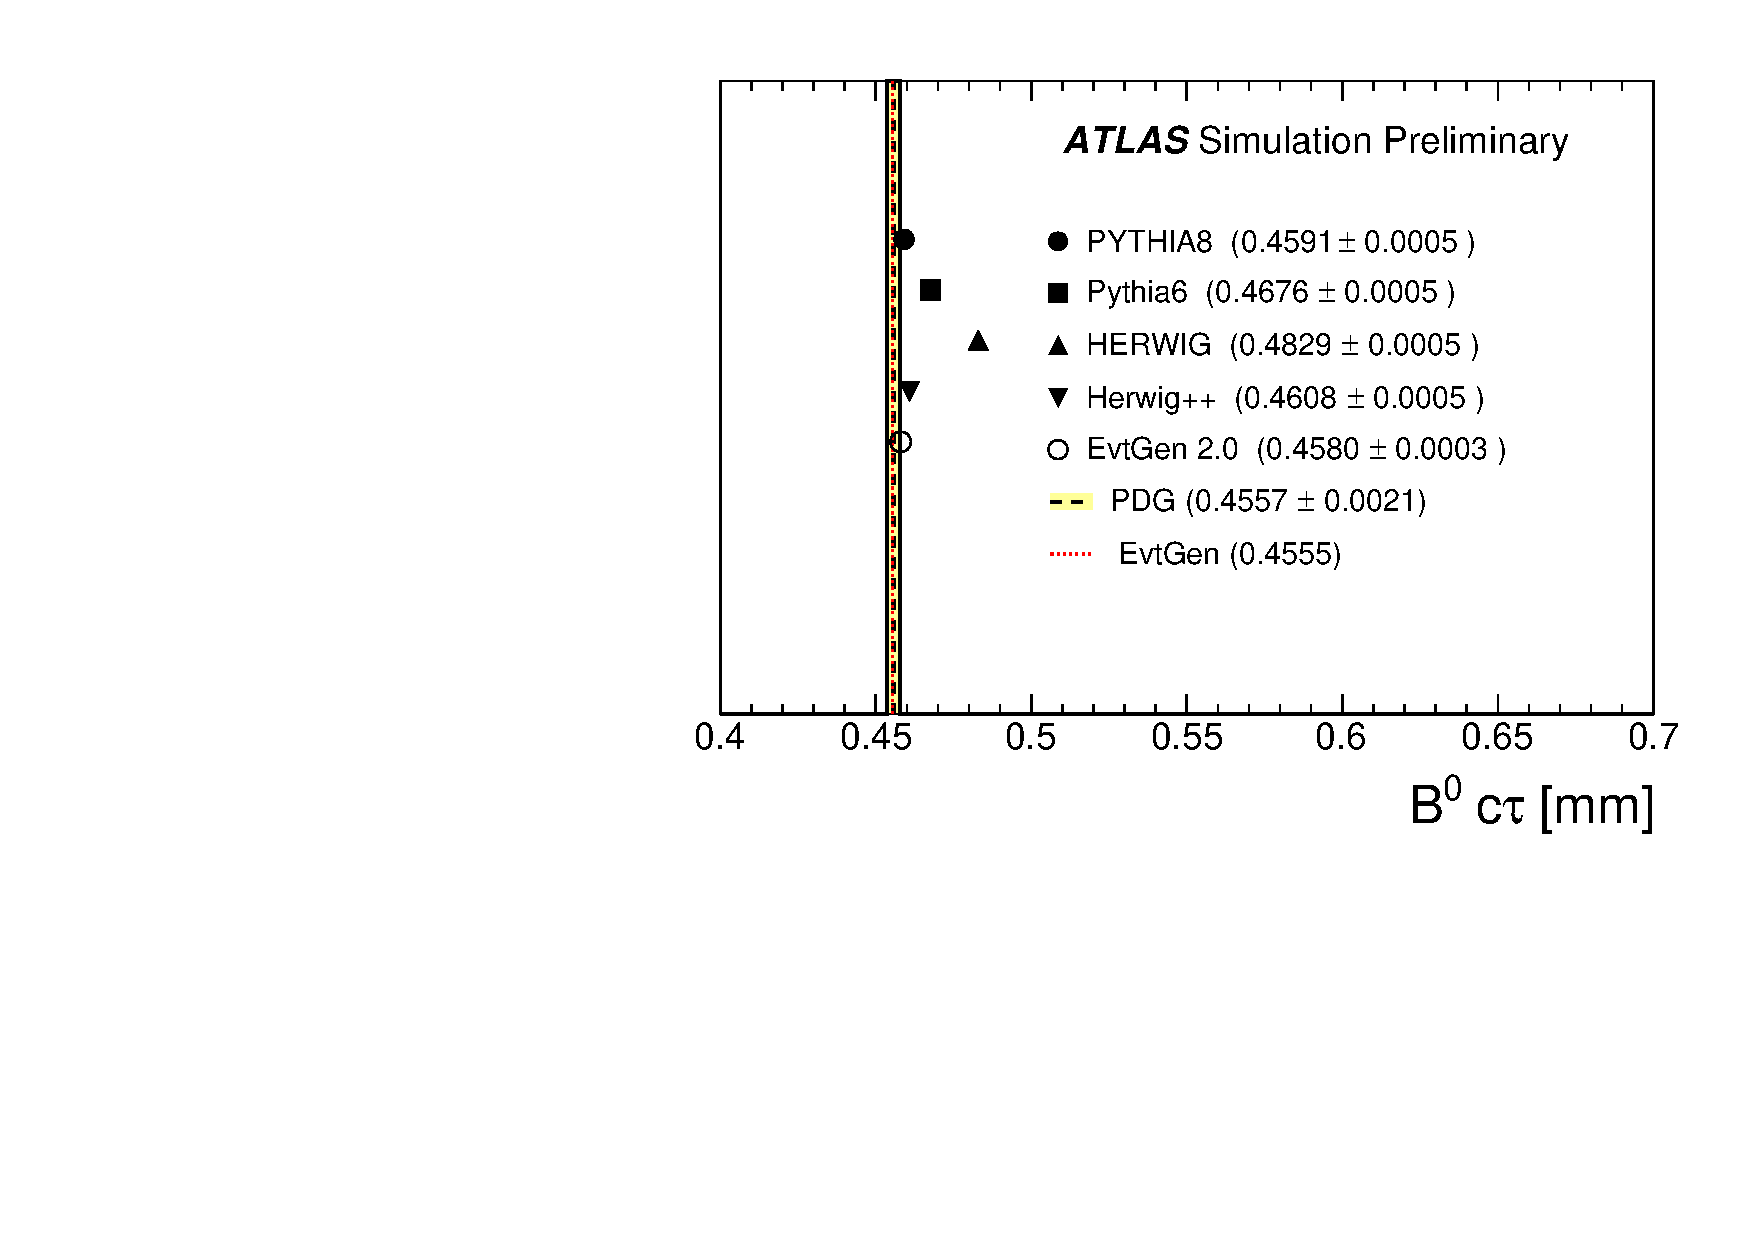
\includegraphics[width=\textwidth]{evtgen/figures/EvtGen/h_B0_life.pdf}
\end{subfigure}
\begin{subfigure}[]{0.45\textwidth}
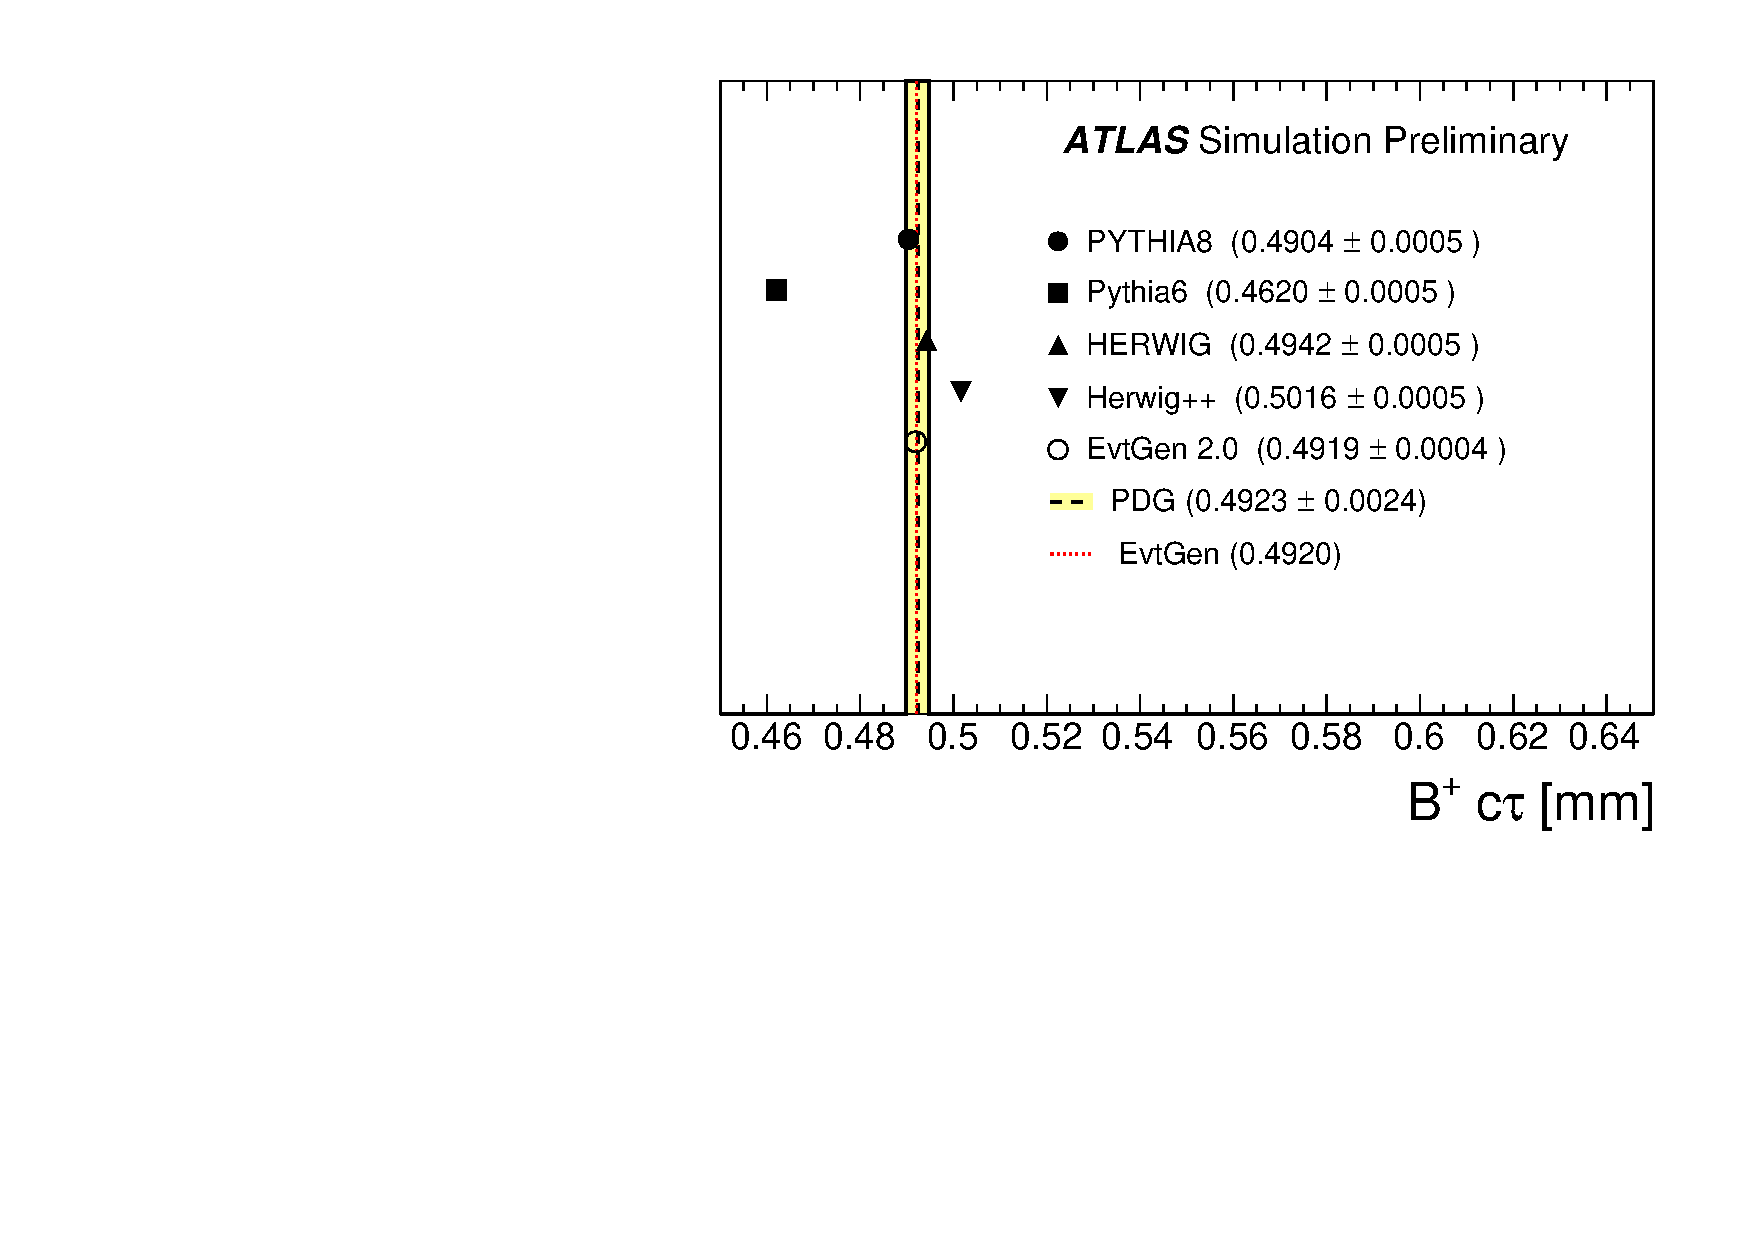
\includegraphics[width=\textwidth]{evtgen/figures/EvtGen/h_B_life.pdf}
\end{subfigure}
\begin{subfigure}[]{0.45\textwidth}
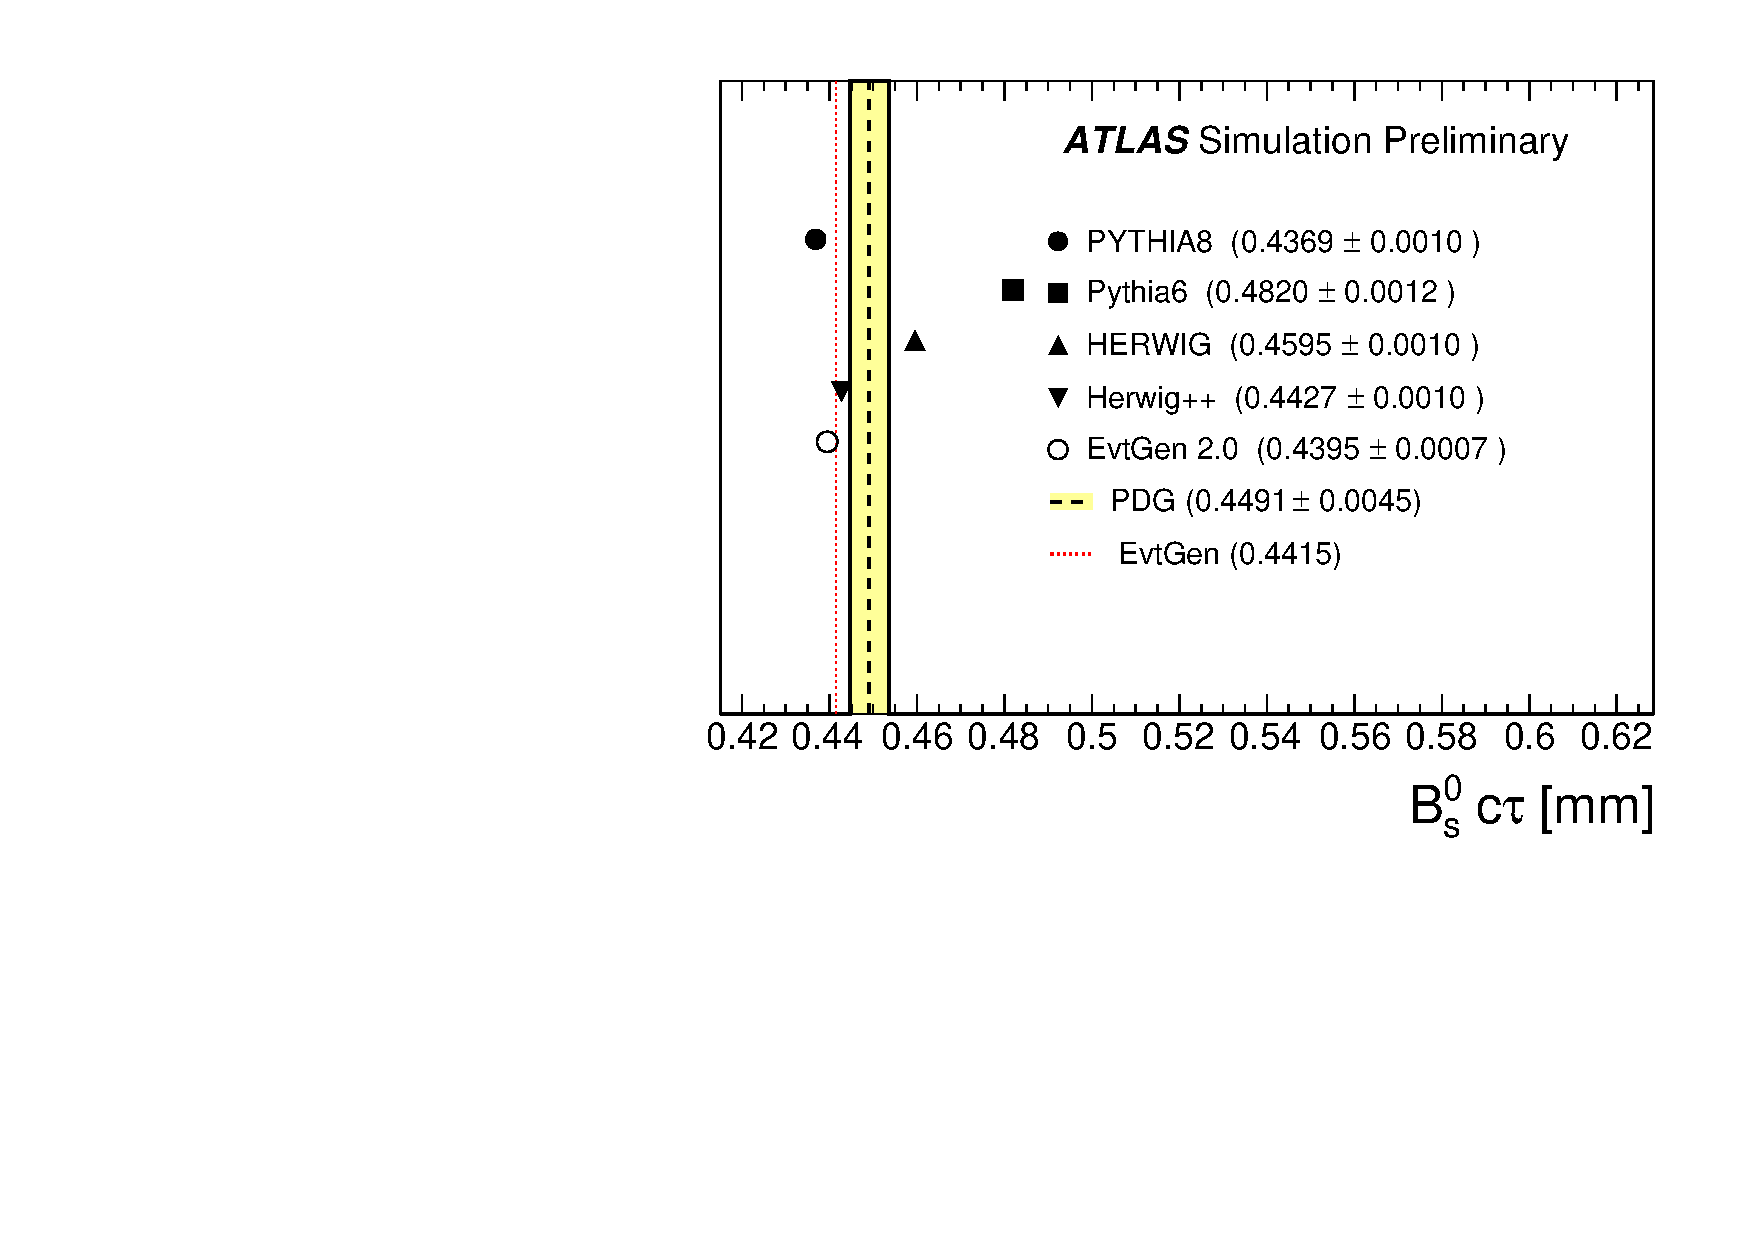
\includegraphics[width=\textwidth]{evtgen/figures/EvtGen/h_Bs_life.pdf}
\end{subfigure}
\begin{subfigure}[]{0.45\textwidth}
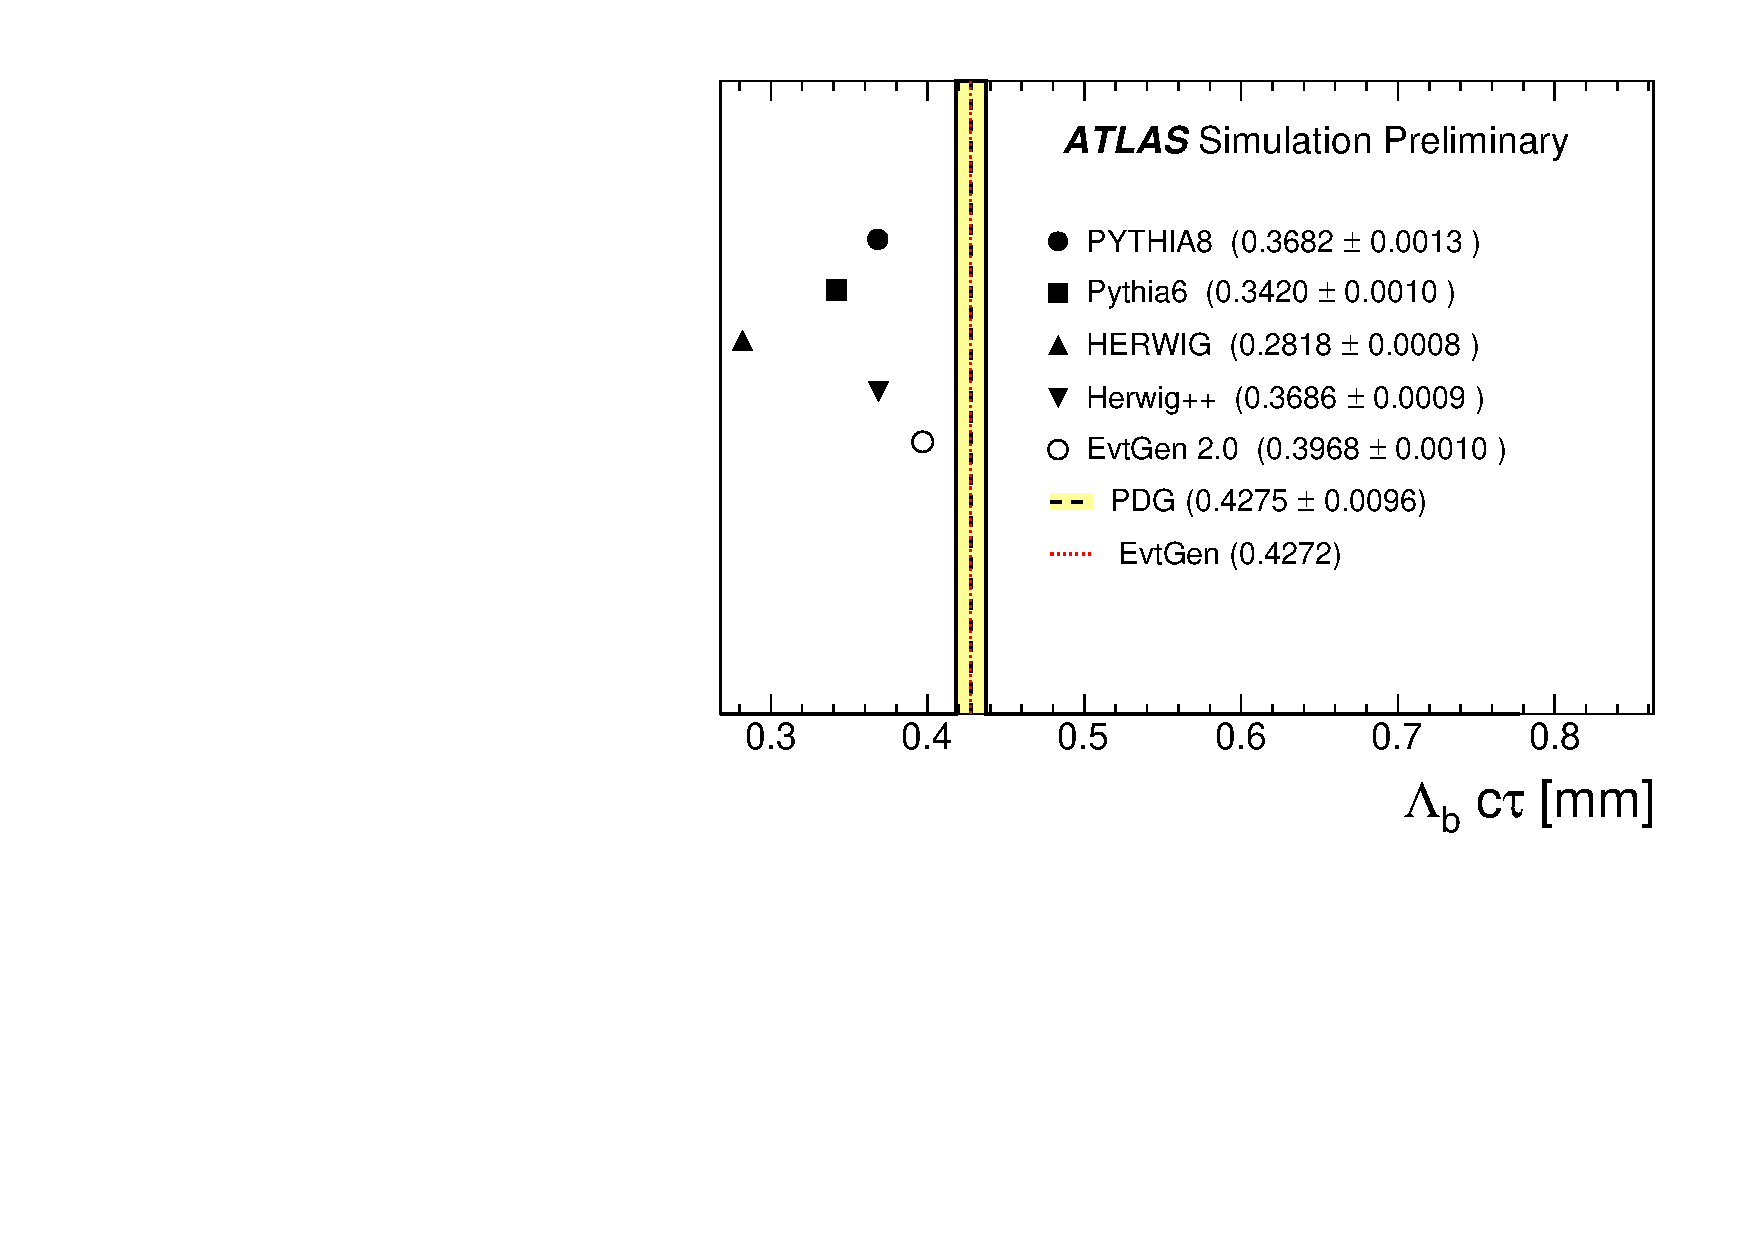
\includegraphics[width=\textwidth]{evtgen/figures/EvtGen/h_Lambdab_life.pdf}
\end{subfigure}
\caption{Comparison of lifetimes of the weakly decaying bottom hadrons 
(a) \Bo,~ (b) \Bp,~ (c) \Bs~ and (d) \Lb~
for four different generators,
\Pythia\ version 427.2, \PythiaE\ version 175, \Herwigpp\  version 2.6.3 and \Herwig\ version 6.520.2, 
both with and without
\EvtGen.  
\EvtGen\ version 2.0 is used with the particle properties table provided with \EvtGen\ and with 
its standard inclusive decay table DECAY\_2010.DEC.
%Adding \EvtGen\ improves agreement of lifetimes with the PDG value. 
The value of the $B_s^0$ lifetime in this default \EvtGen\ particle properties table 
differs from the world average listed by the PDG~\cite{PhysRevD.86.010001}.}
\label{fig:blife}
\end{figure}

\begin{figure}
\centering
\begin{subfigure}[]{0.45\textwidth}
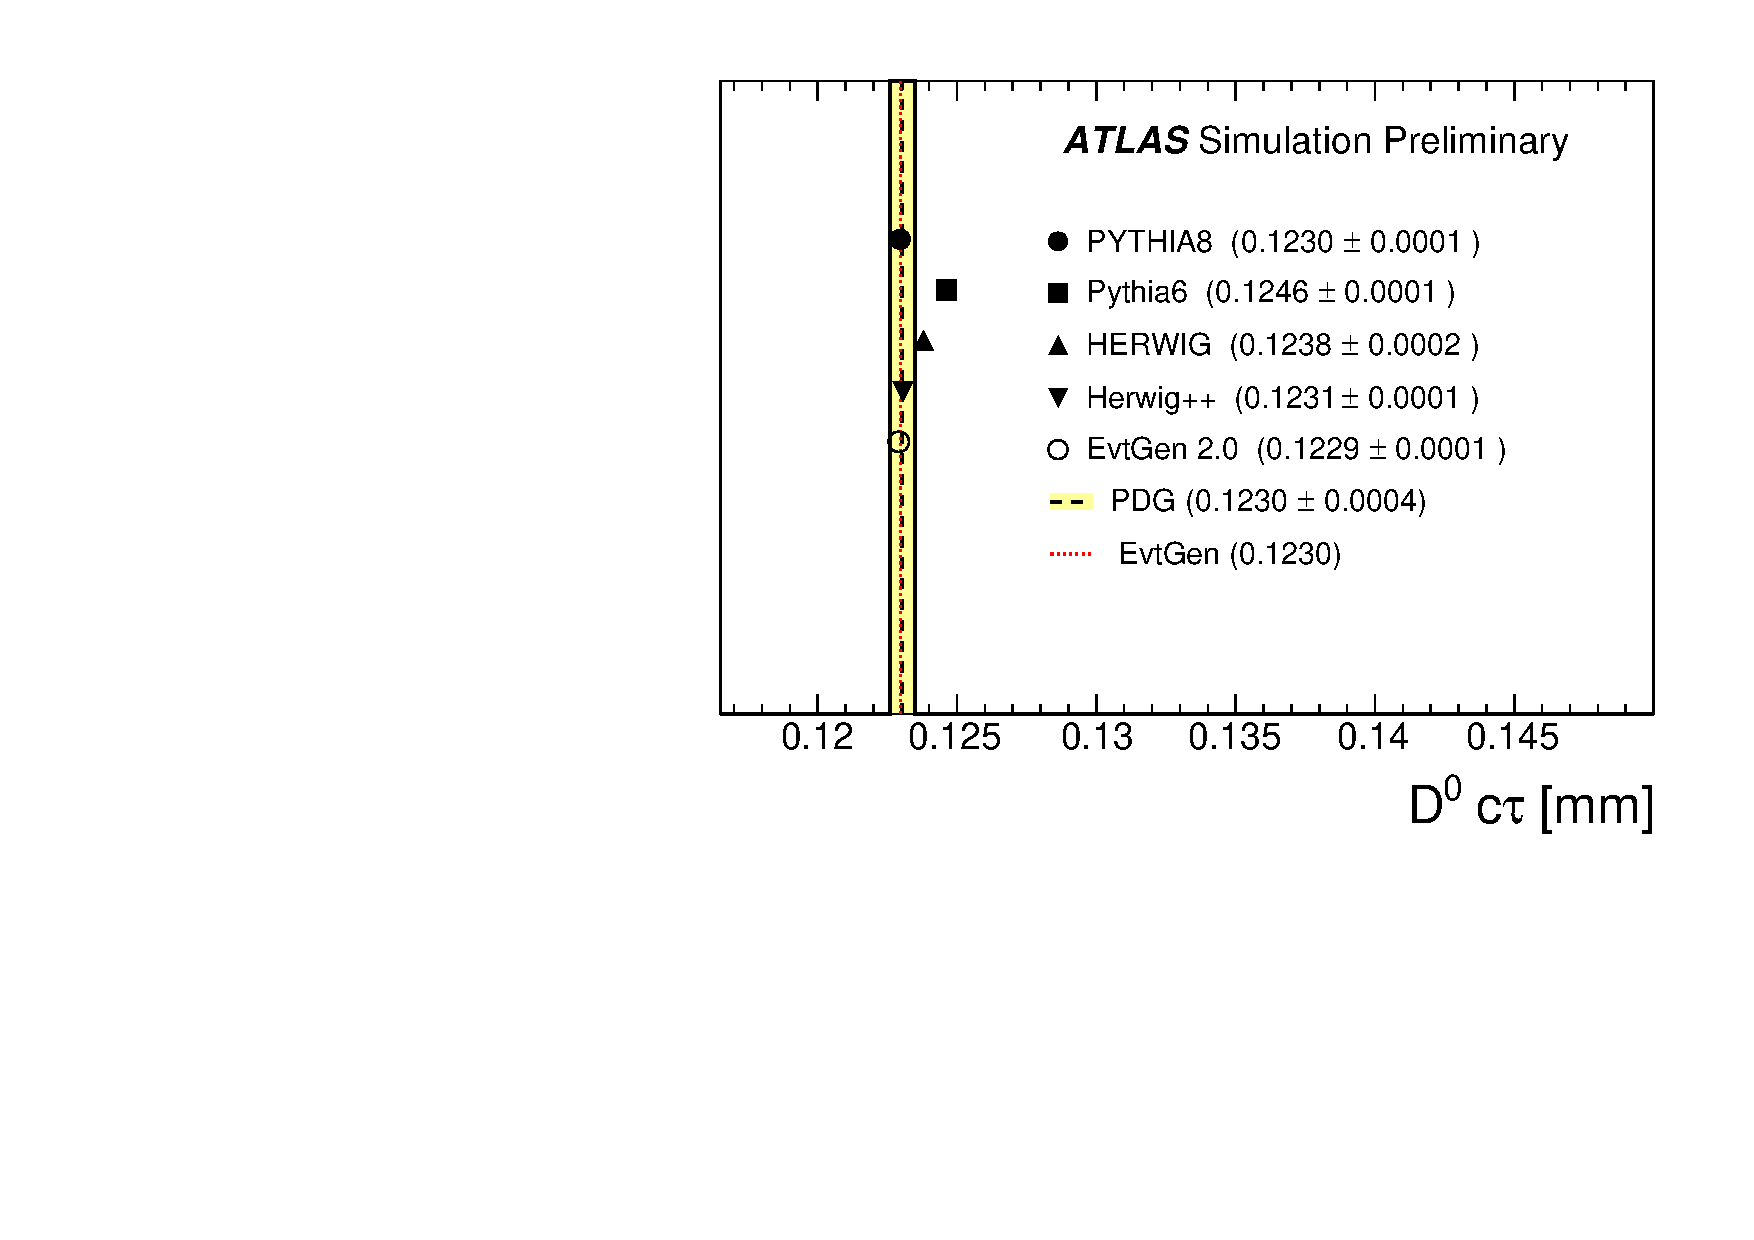
\includegraphics[width=\textwidth]{evtgen/figures/EvtGen/h_D0_life.pdf}
\end{subfigure}
\begin{subfigure}[]{0.45\textwidth}
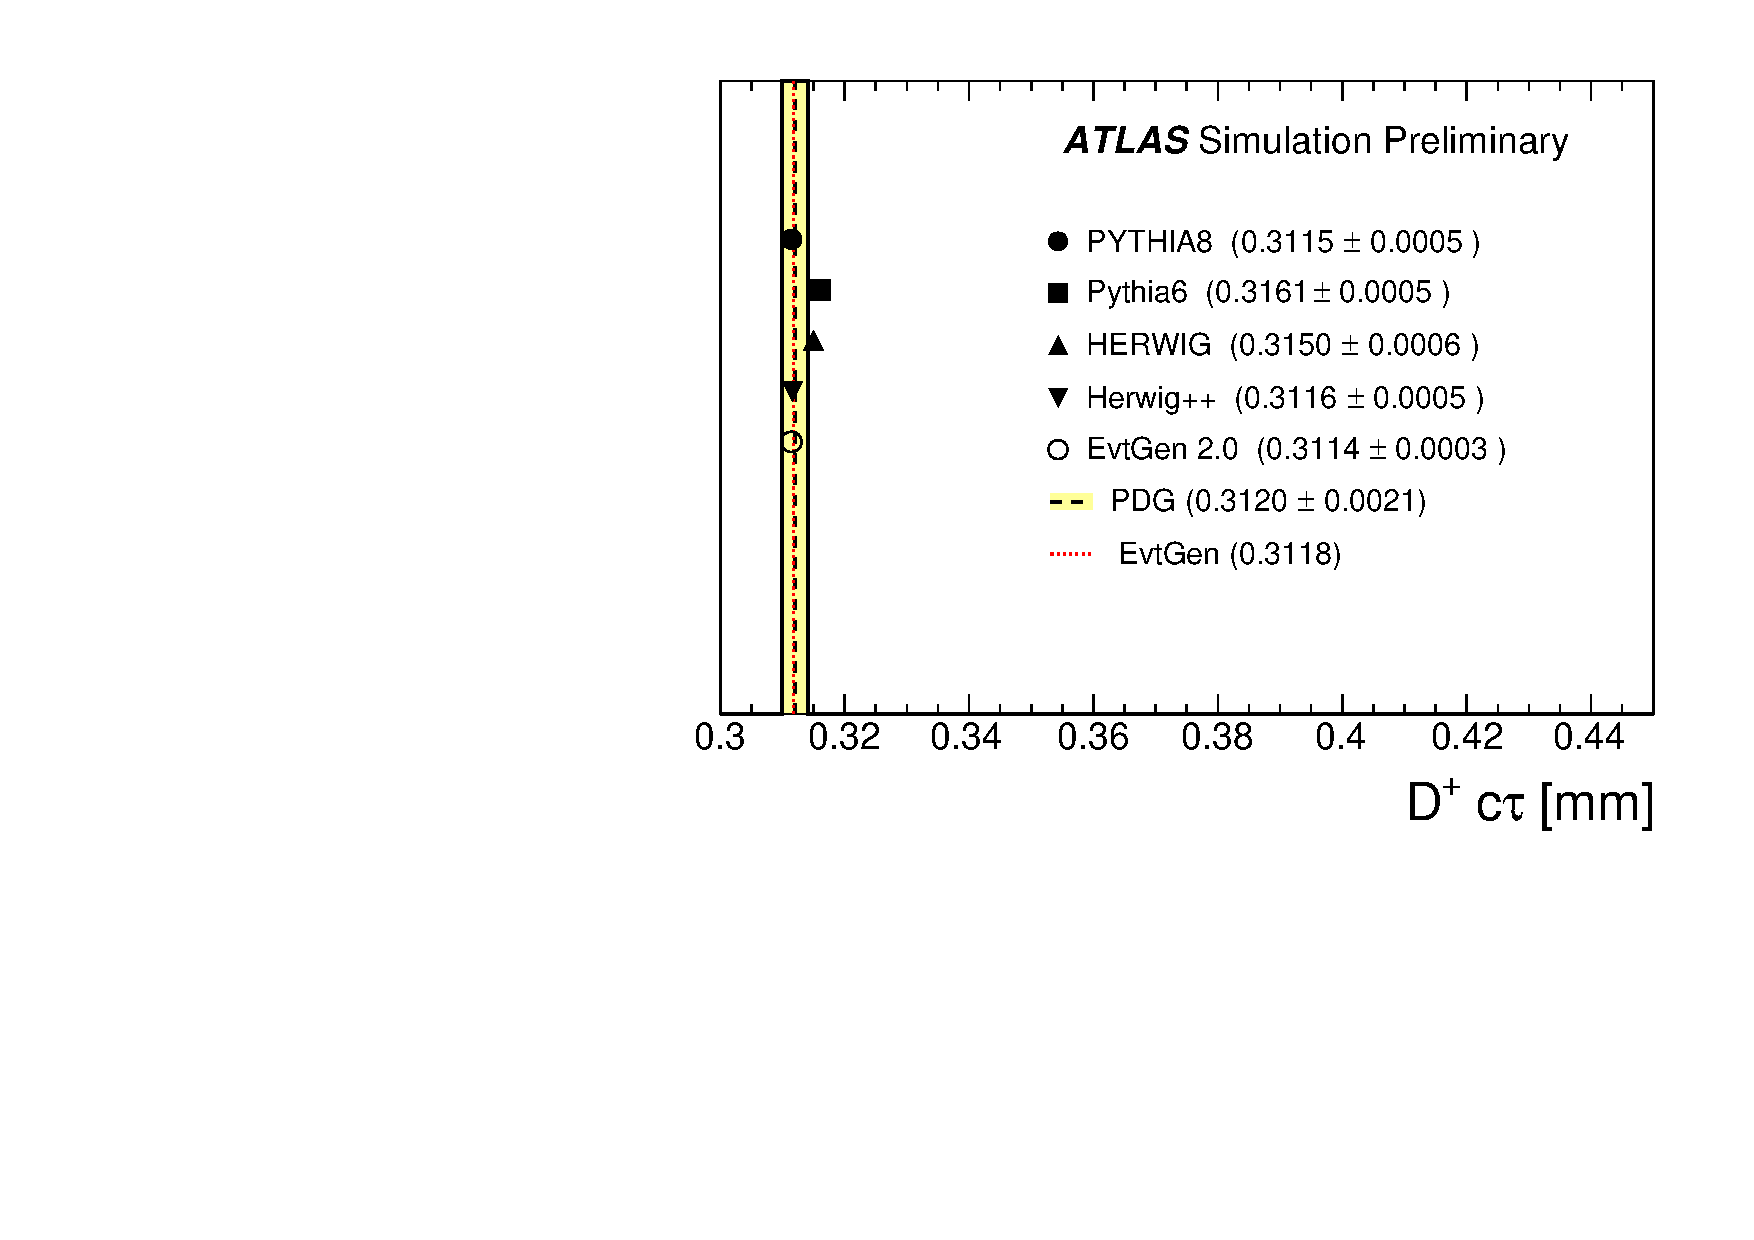
\includegraphics[width=\textwidth]{evtgen/figures/EvtGen/h_D_life.pdf}
\end{subfigure}\\
\begin{subfigure}[]{0.45\textwidth}
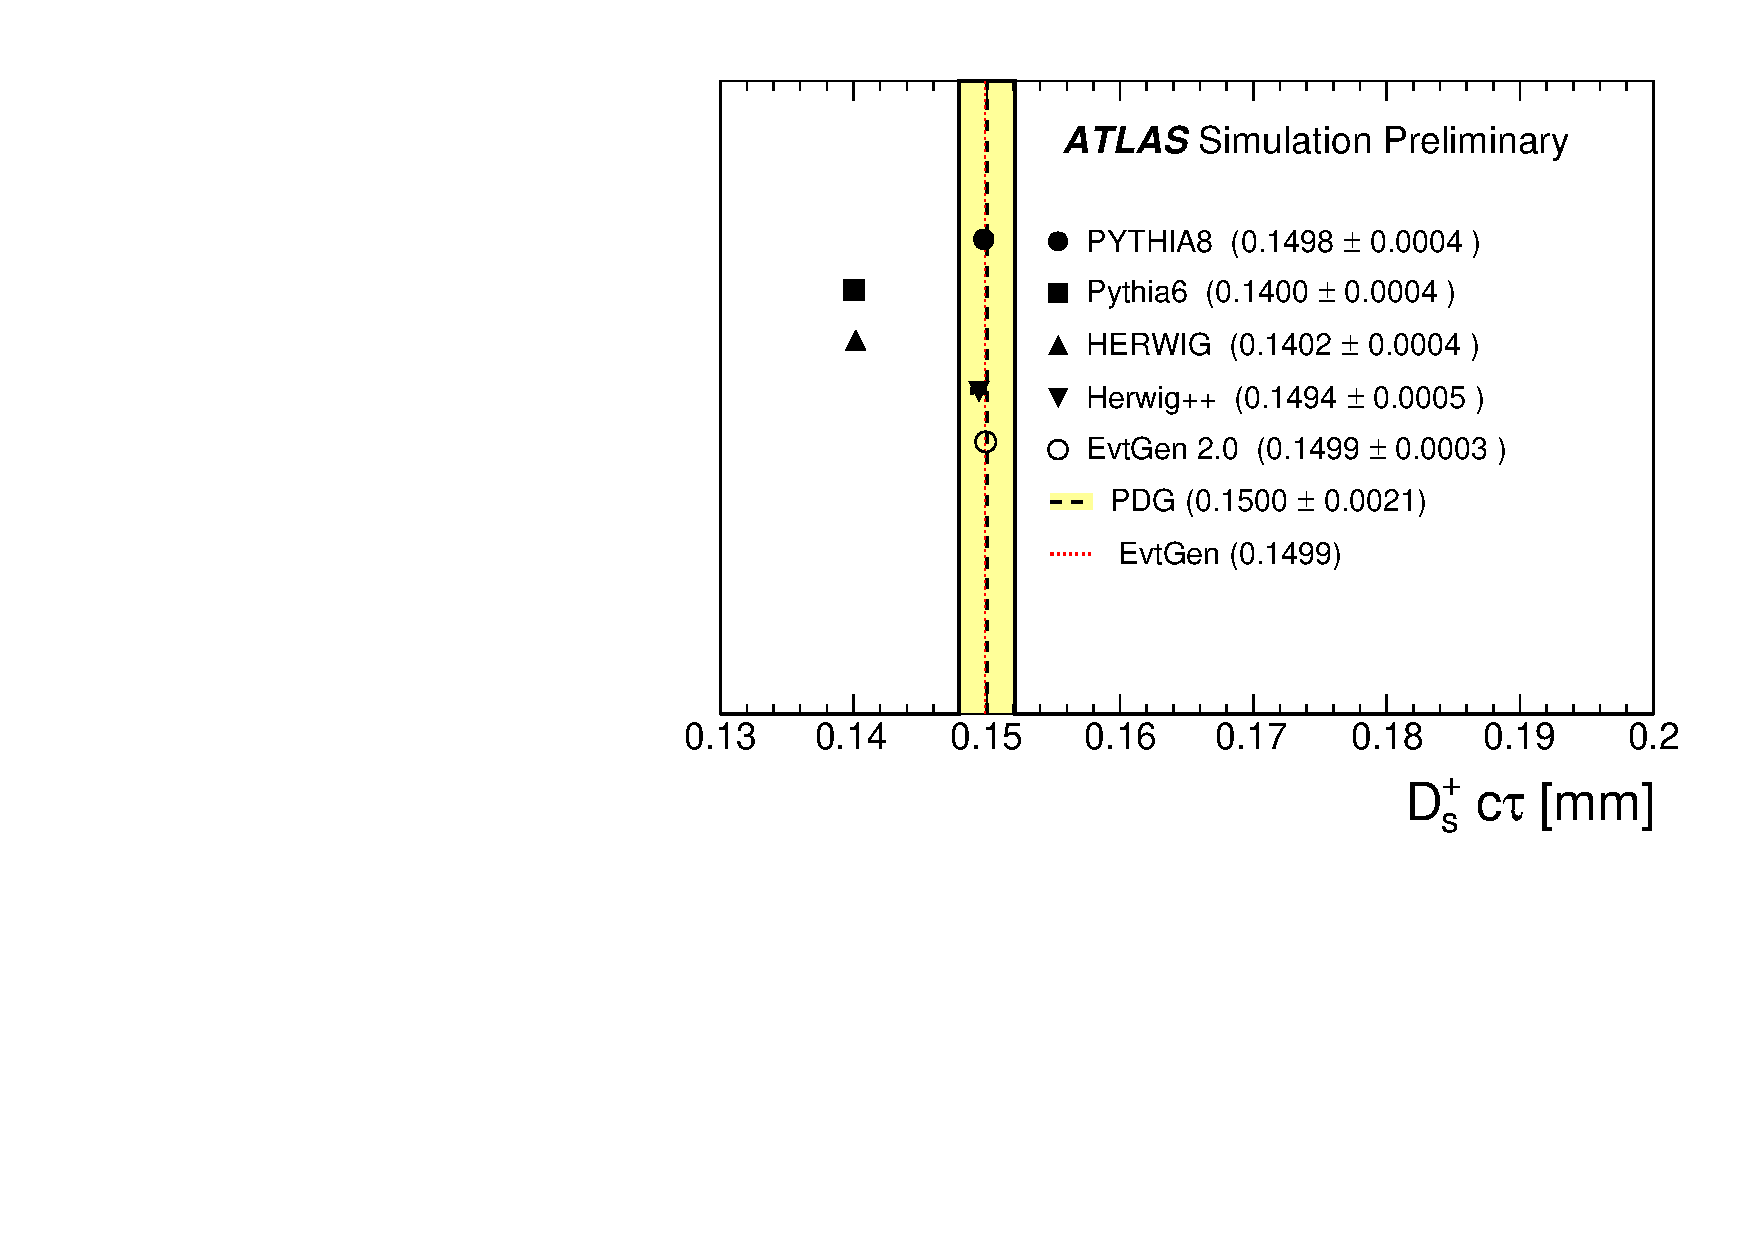
\includegraphics[width=\textwidth]{evtgen/figures/EvtGen/h_Ds_life.pdf}
\end{subfigure}
\begin{subfigure}[]{0.45\textwidth}
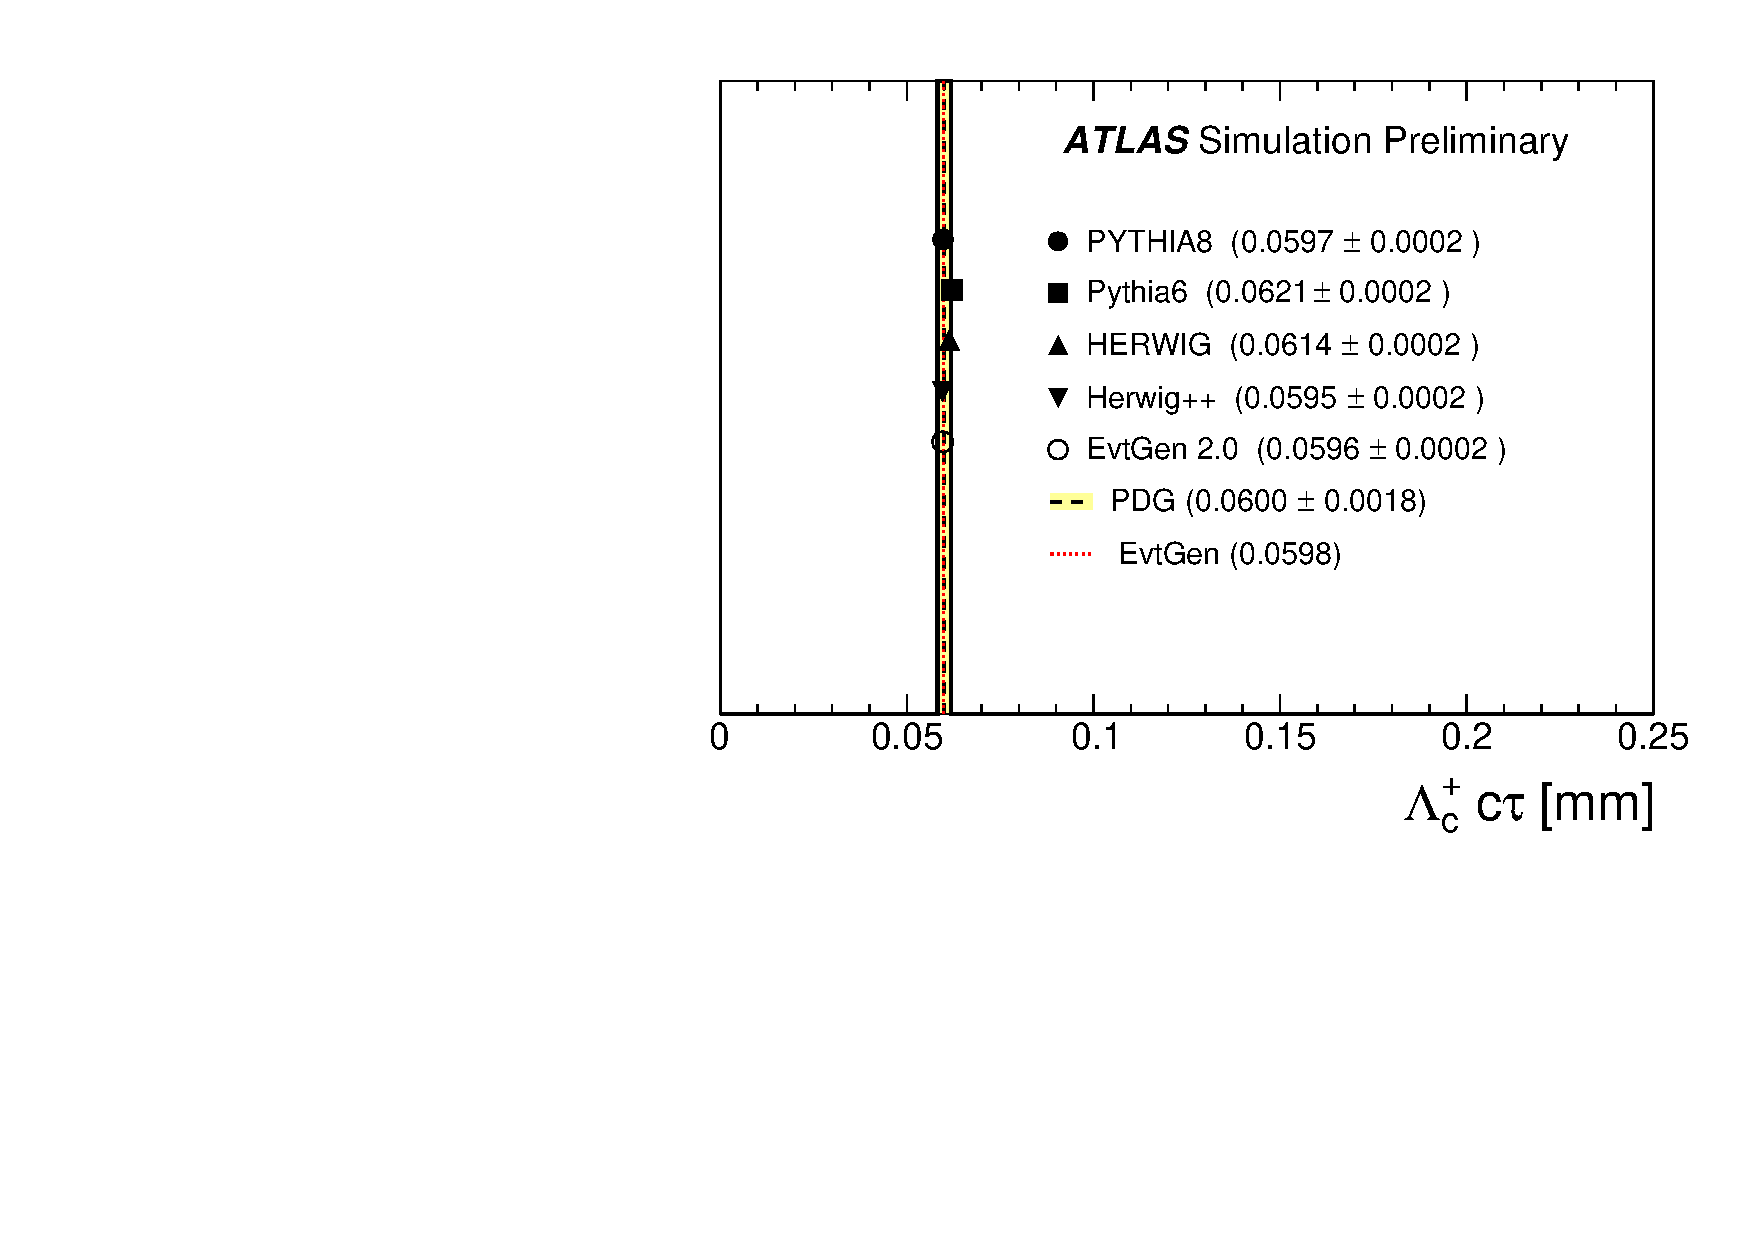
\includegraphics[width=\textwidth]{evtgen/figures/EvtGen/h_Lambdac_life.pdf}
\end{subfigure}
\caption{Comparison of lifetimes of the weakly decaying charm hadrons 
(a) \Dzero, (b) \Dplus, (c) \Ds\ and (d) \Lc~
in four different generators,
\Pythia\ version 427.2, \PythiaE\ version 175, \Herwigpp\  version 2.6.3 and \Herwig\ version 6.520.2, 
both with and without
\EvtGen.  
\EvtGen\ version 2.0 is used with the particle properties table provided with \EvtGen\ and with 
its standard inclusive decay table DECAY\_2010.DEC.
}
\label{fig:clife}
\end{figure}


\begin{figure}
\centering
\begin{subfigure}[]{0.45\textwidth}
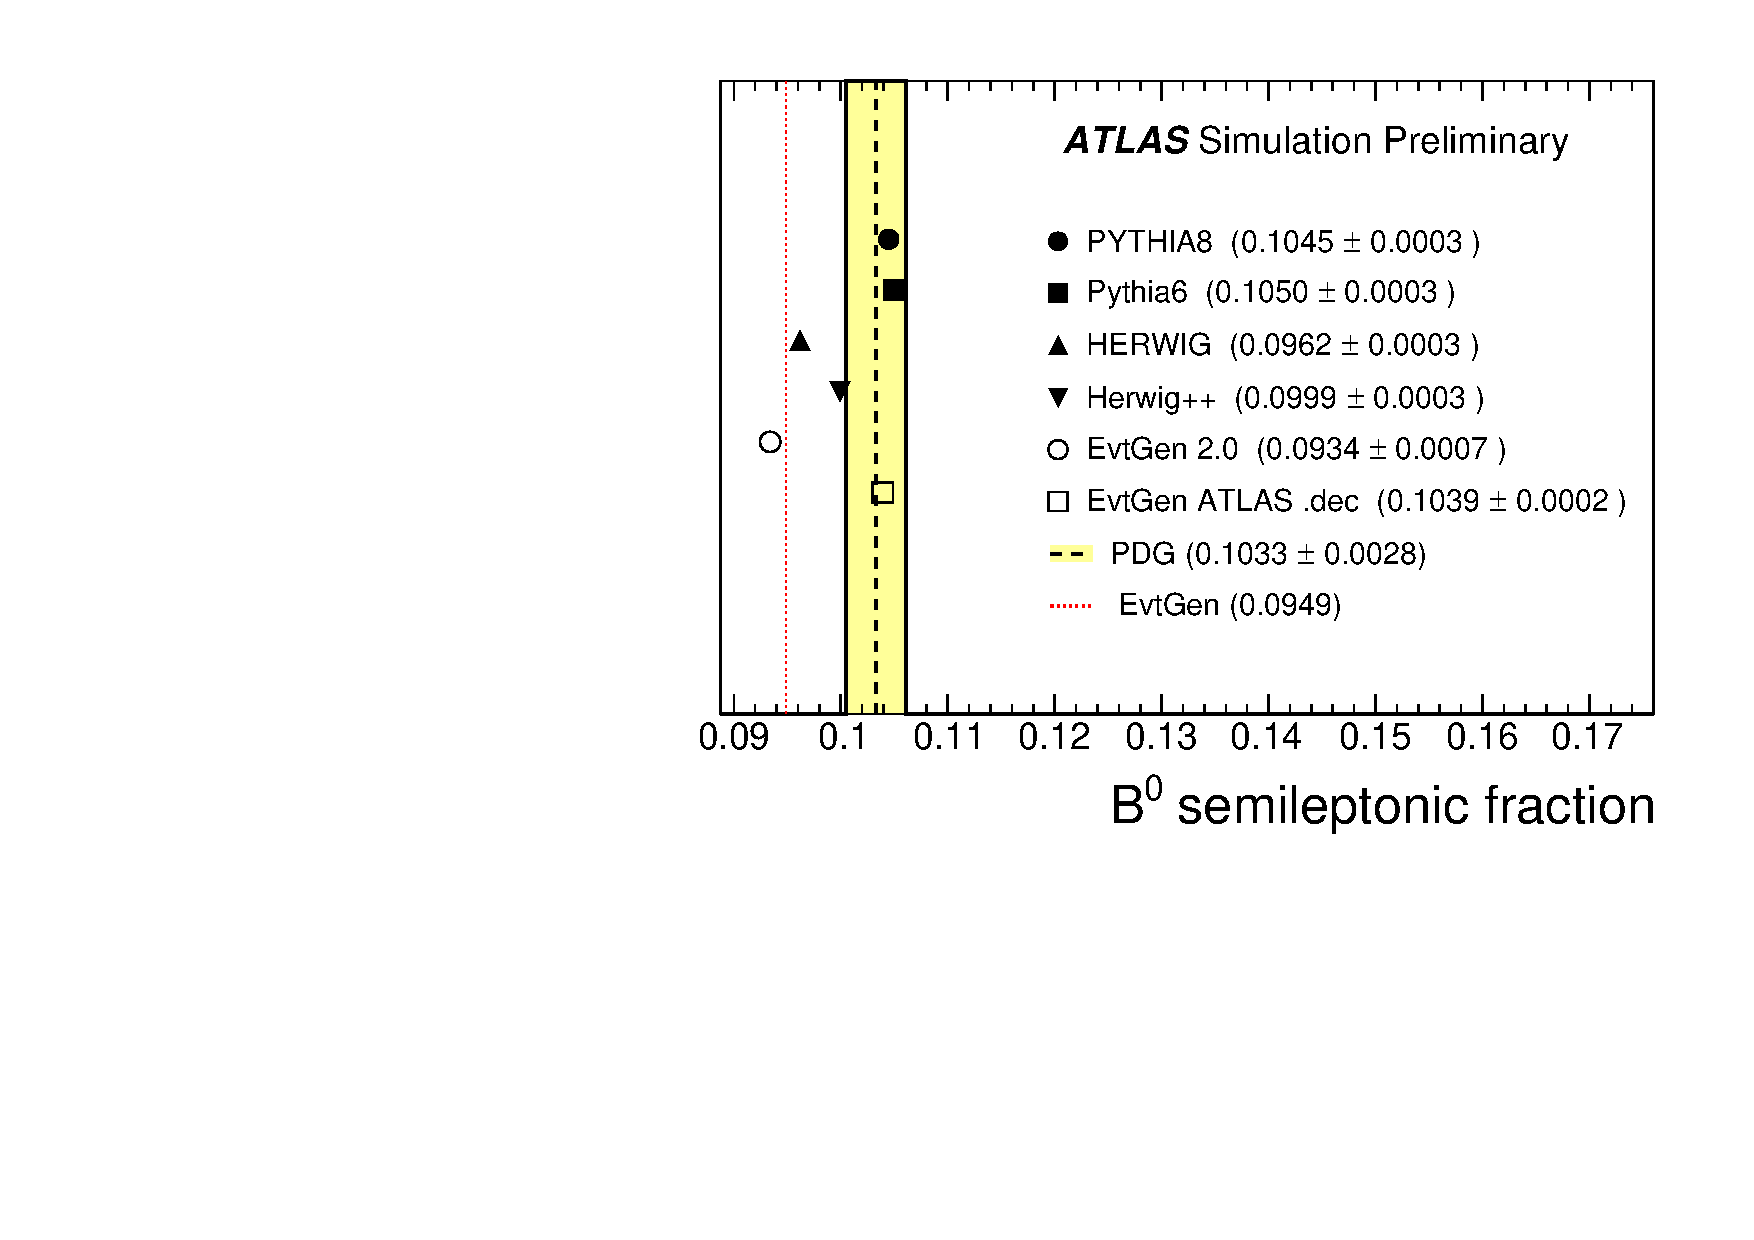
\includegraphics[width=\textwidth]{evtgen/figures/EvtGen/h_B0_sl.pdf}
\end{subfigure}
\begin{subfigure}[]{0.45\textwidth}
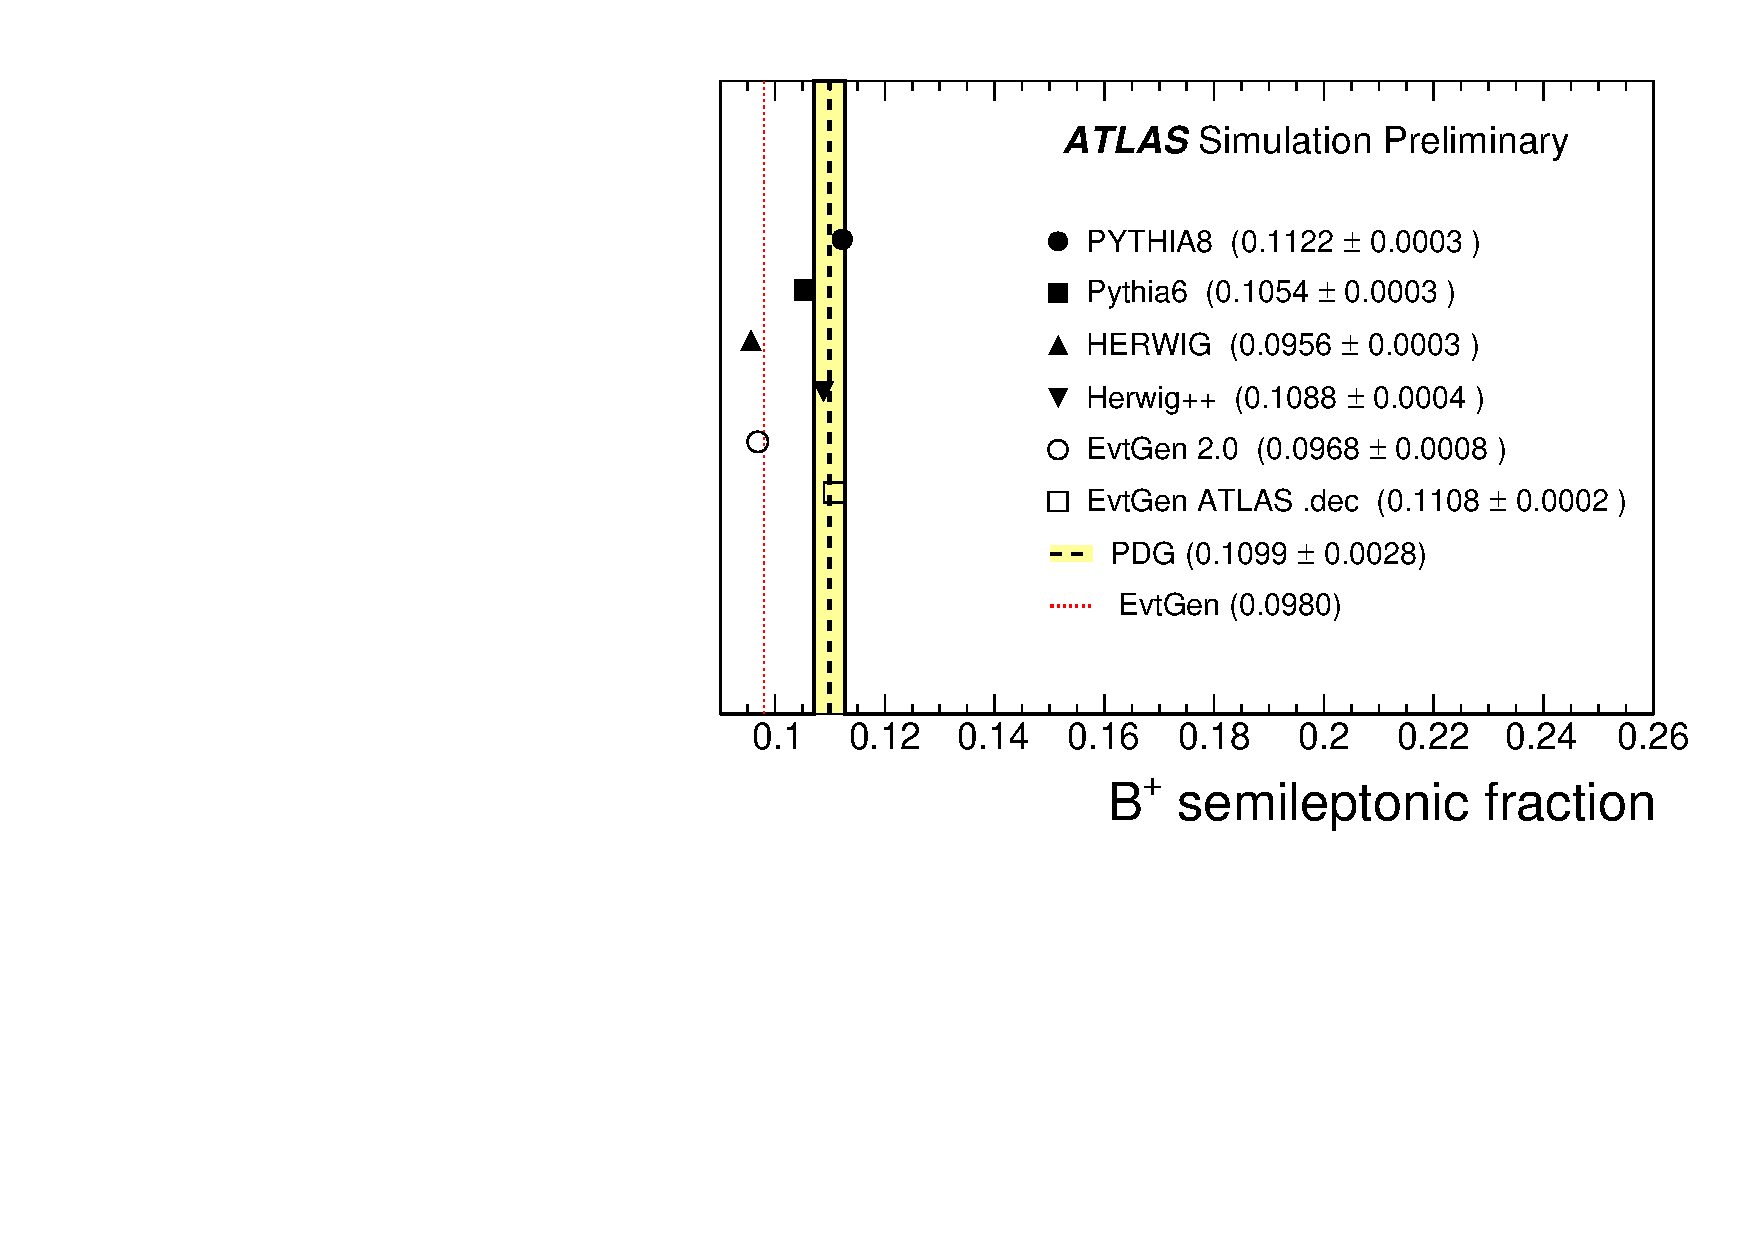
\includegraphics[width=\textwidth]{evtgen/figures/EvtGen/h_B_sl.pdf}
\end{subfigure}
\begin{subfigure}[]{0.45\textwidth}
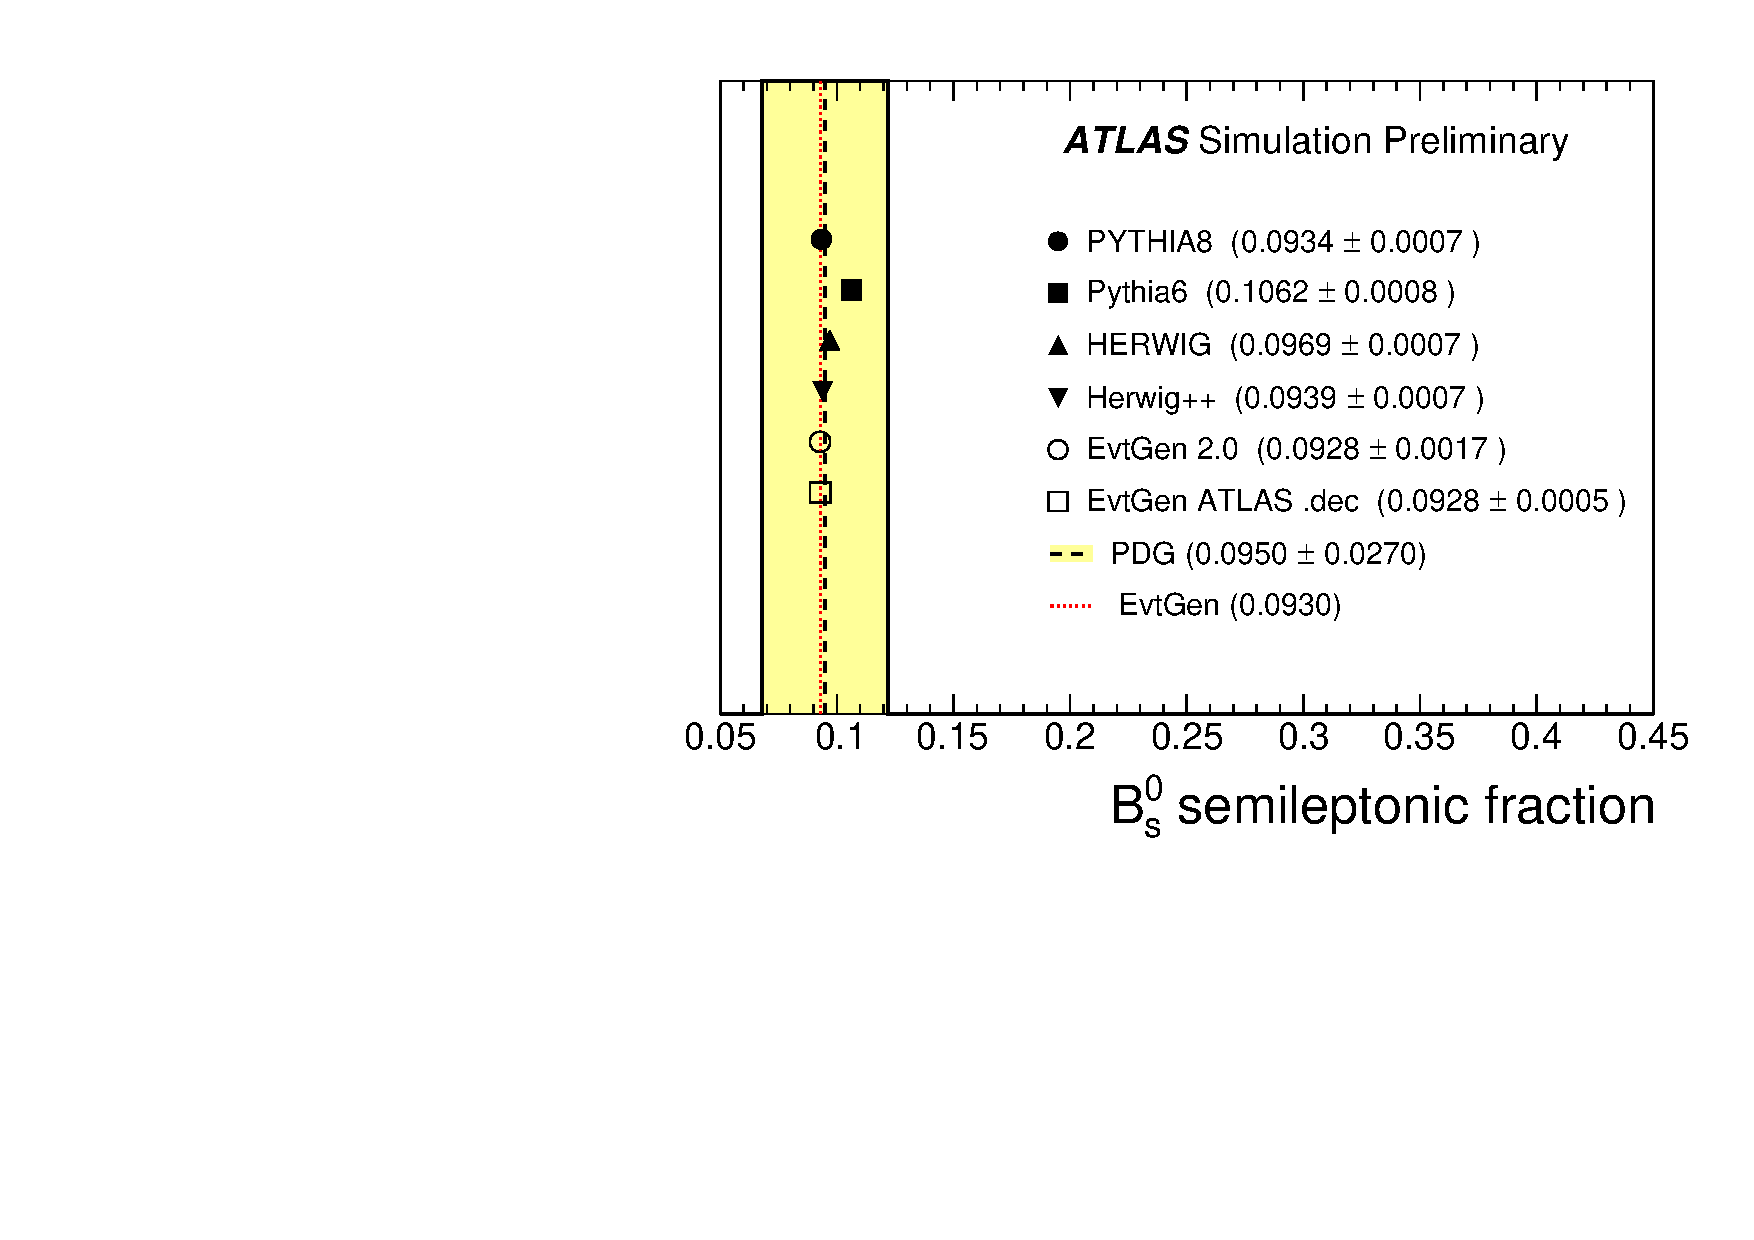
\includegraphics[width=\textwidth]{evtgen/figures/EvtGen/h_Bs_sl.pdf}
\end{subfigure}
\begin{subfigure}[]{0.45\textwidth}
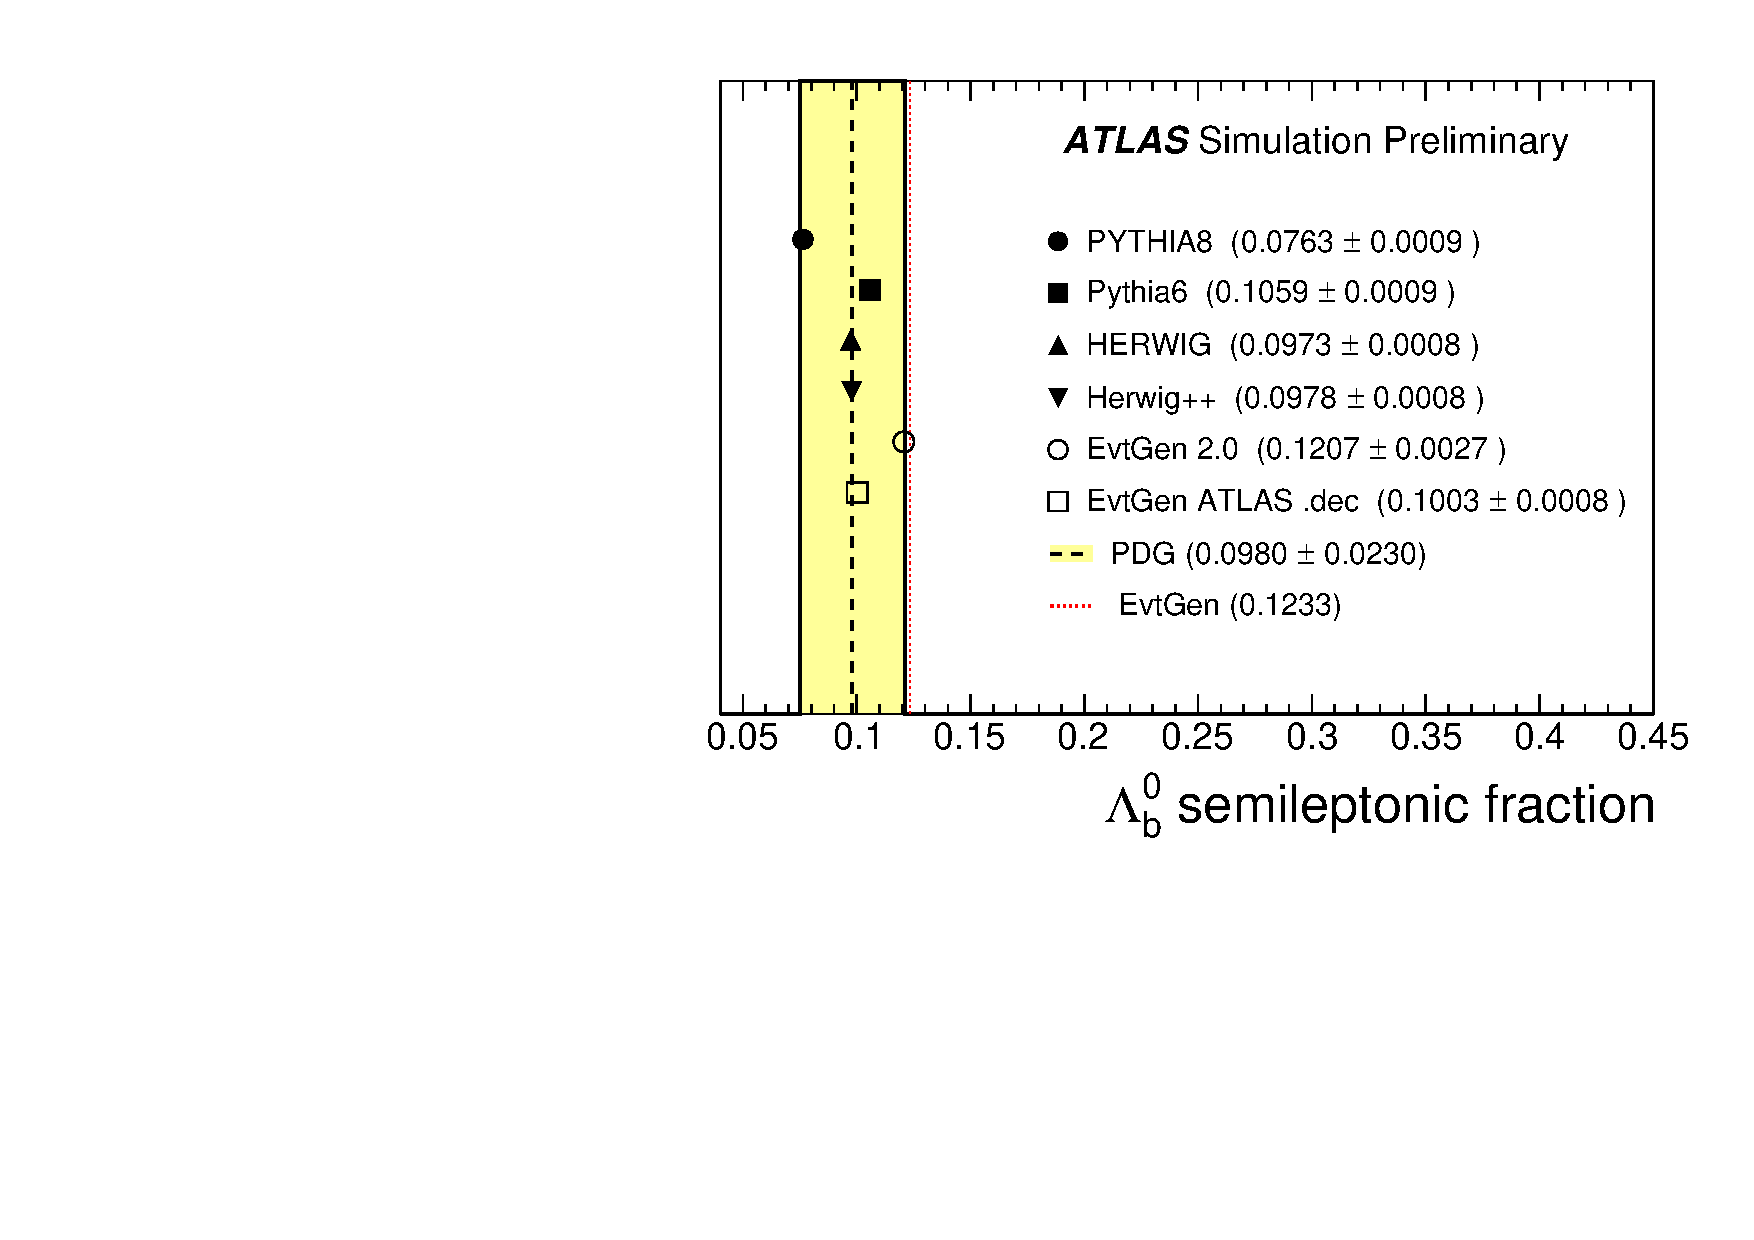
\includegraphics[width=\textwidth]{evtgen/figures/EvtGen/h_Lambdab_sl.pdf}
\end{subfigure}
\caption{Comparison of semileptonic branching fraction $B\rightarrow e^-\overline{\nu_e} X$ 
of the weakly decaying bottom hadrons 
(a) \Bo, (b) \Bp, (c) \Bs~ and (d) \Lb~
in four different generators,
%Adding \EvtGen\ improves agreement with the PDG value. 
\Pythia\ version 427.2, \PythiaE\ version 175, \Herwigpp\  version 2.6.3 and \Herwig\ version 6.520.2, 
both with and without
\EvtGen.  
\EvtGen\ version 2.0 is used with the particle properties table provided with \EvtGen\ and with 
its standard inclusive decay table DECAY\_2010.DEC, as well as a custom decay table with developed for ATLAS with the most up to date semileptonic fractions from the PDG.
Only decays where the electron is the direct decay product of the bottom hadron are included here (e.g.
electrons coming from charm or $\tau $ decays are excluded).
The band shown for the world average branching fractions correspond to the
measured decay fraction for $B\rightarrow e\nu X_c$ listed by the PDG\cite{PhysRevD.86.010001}.
The values of the $B^0$, $B^+$ and $\Lambda^0_b$~semileptonic fractions in the 
default \EvtGen\ particle properties table have been tuned to the
observed inclusive $B\rightarrow D\ell\nu+\mathrm{anything}$ branching fraction, which has a 
larger uncertainty.}
\label{fig:bsl}
\end{figure}

\begin{figure}
\centering
\begin{subfigure}[]{0.45\textwidth}
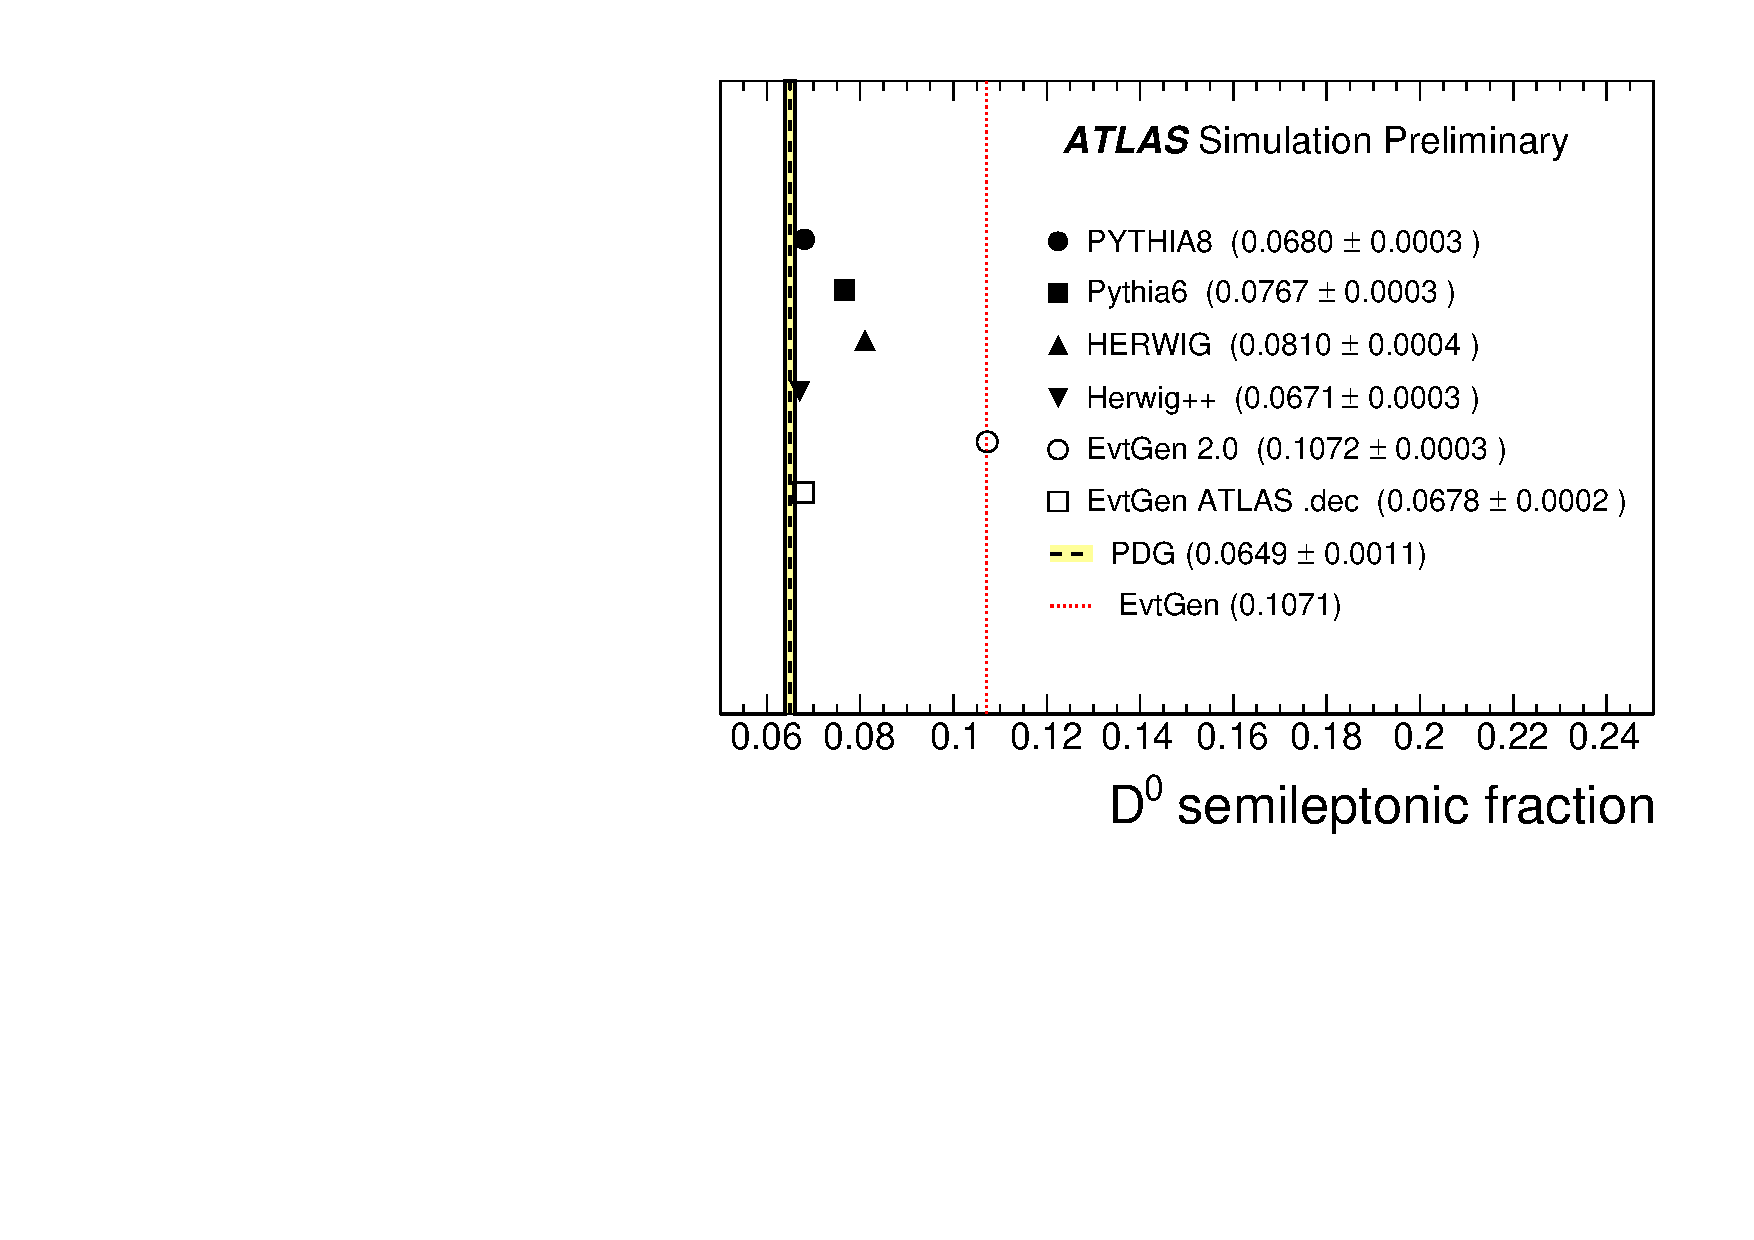
\includegraphics[width=\textwidth]{evtgen/figures/EvtGen/h_D0_sl.pdf}
\end{subfigure}
\begin{subfigure}[]{0.45\textwidth}
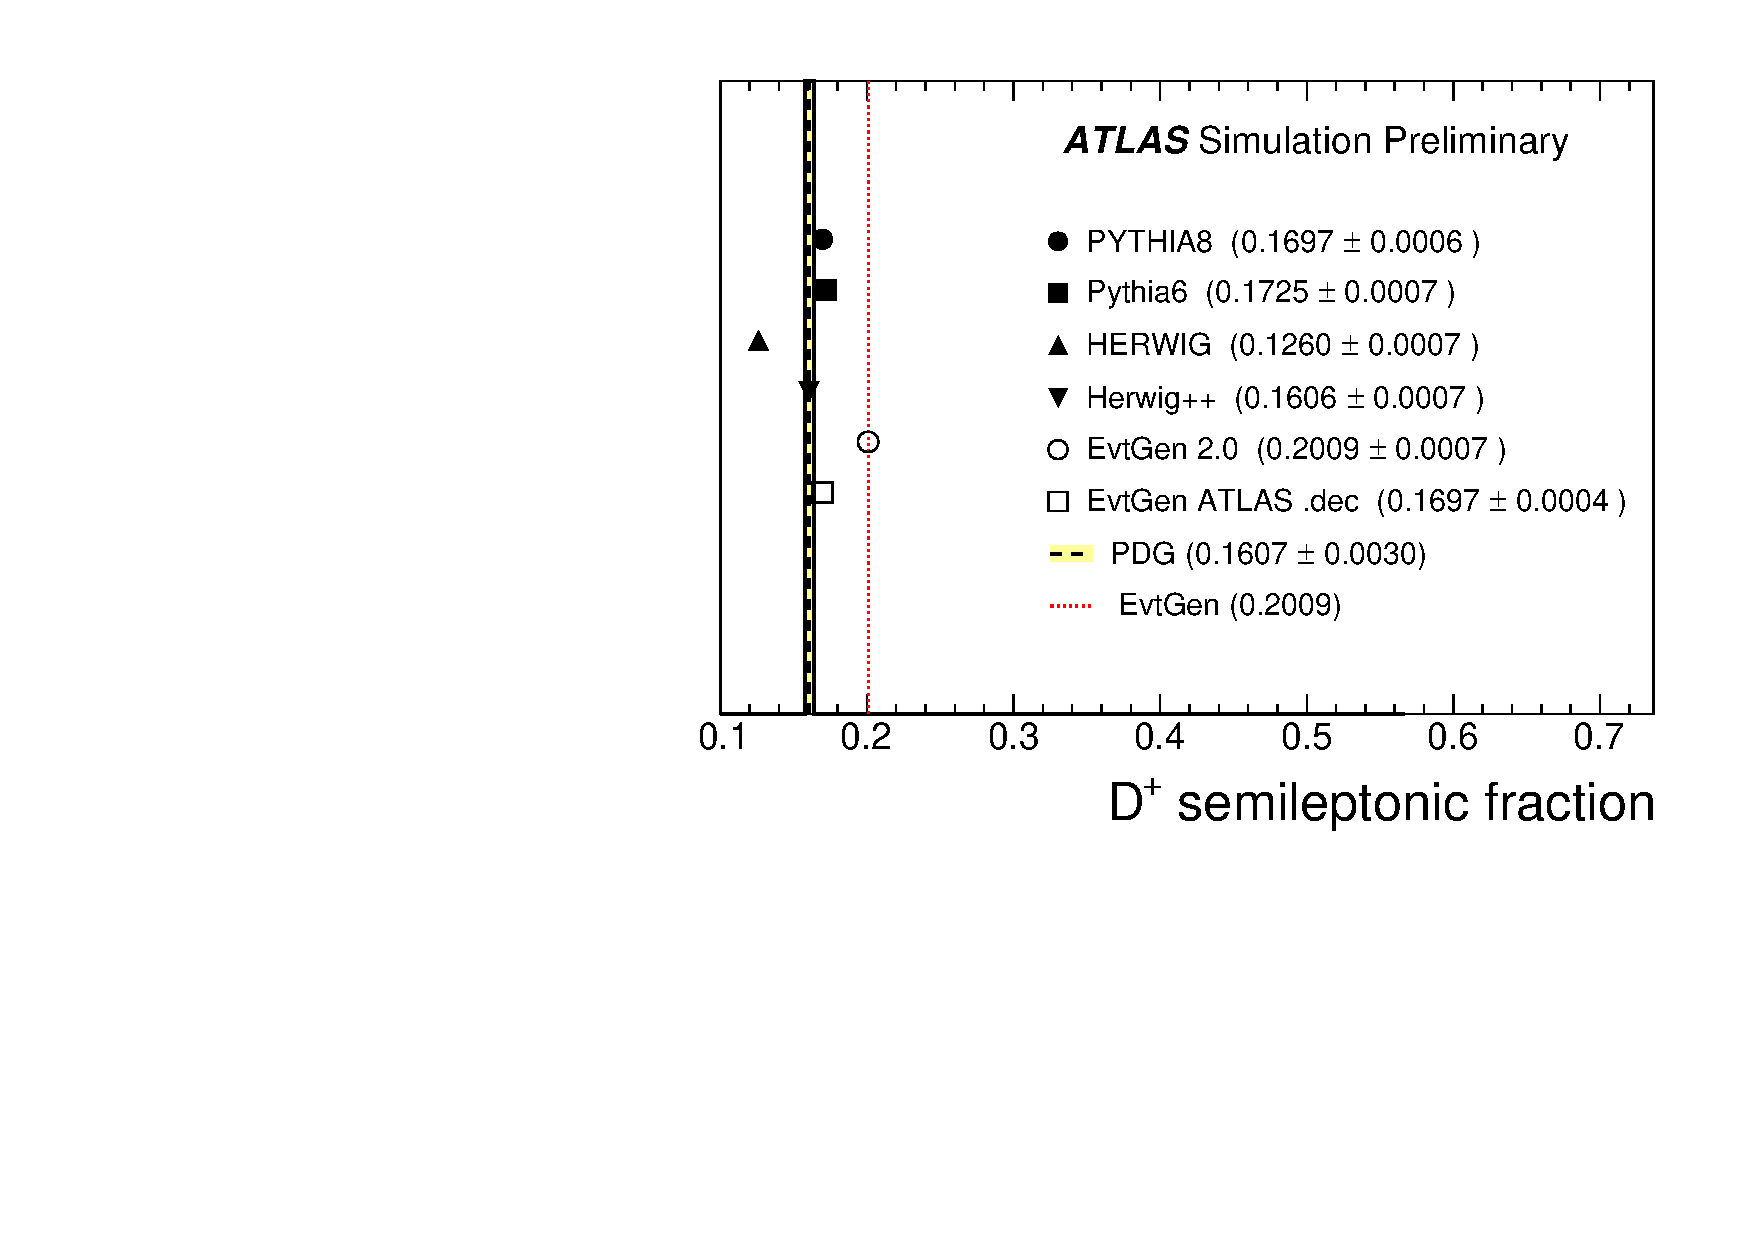
\includegraphics[width=\textwidth]{evtgen/figures/EvtGen/h_D_sl.pdf}
\end{subfigure}
\begin{subfigure}[]{0.45\textwidth}
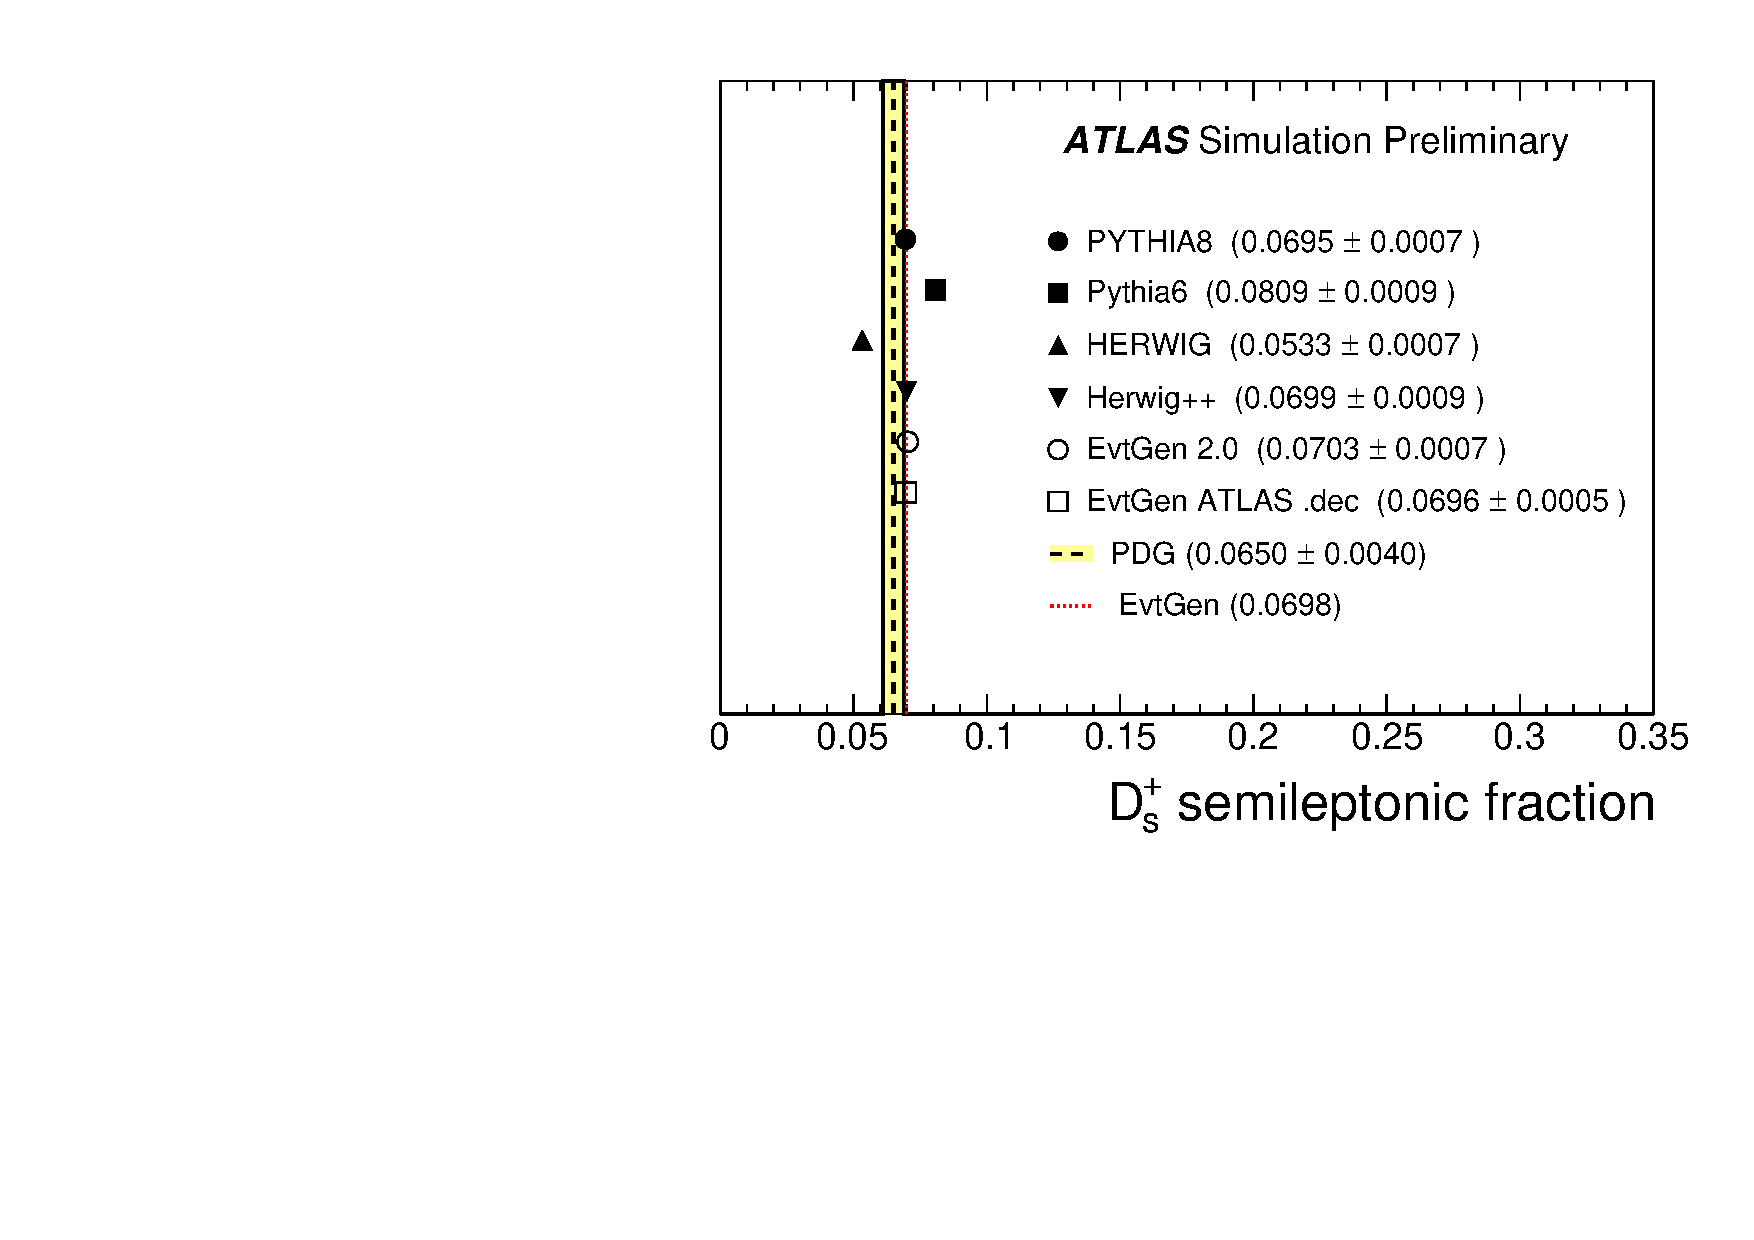
\includegraphics[width=\textwidth]{evtgen/figures/EvtGen/h_Ds_sl.pdf}
\end{subfigure}
\begin{subfigure}[]{0.45\textwidth}
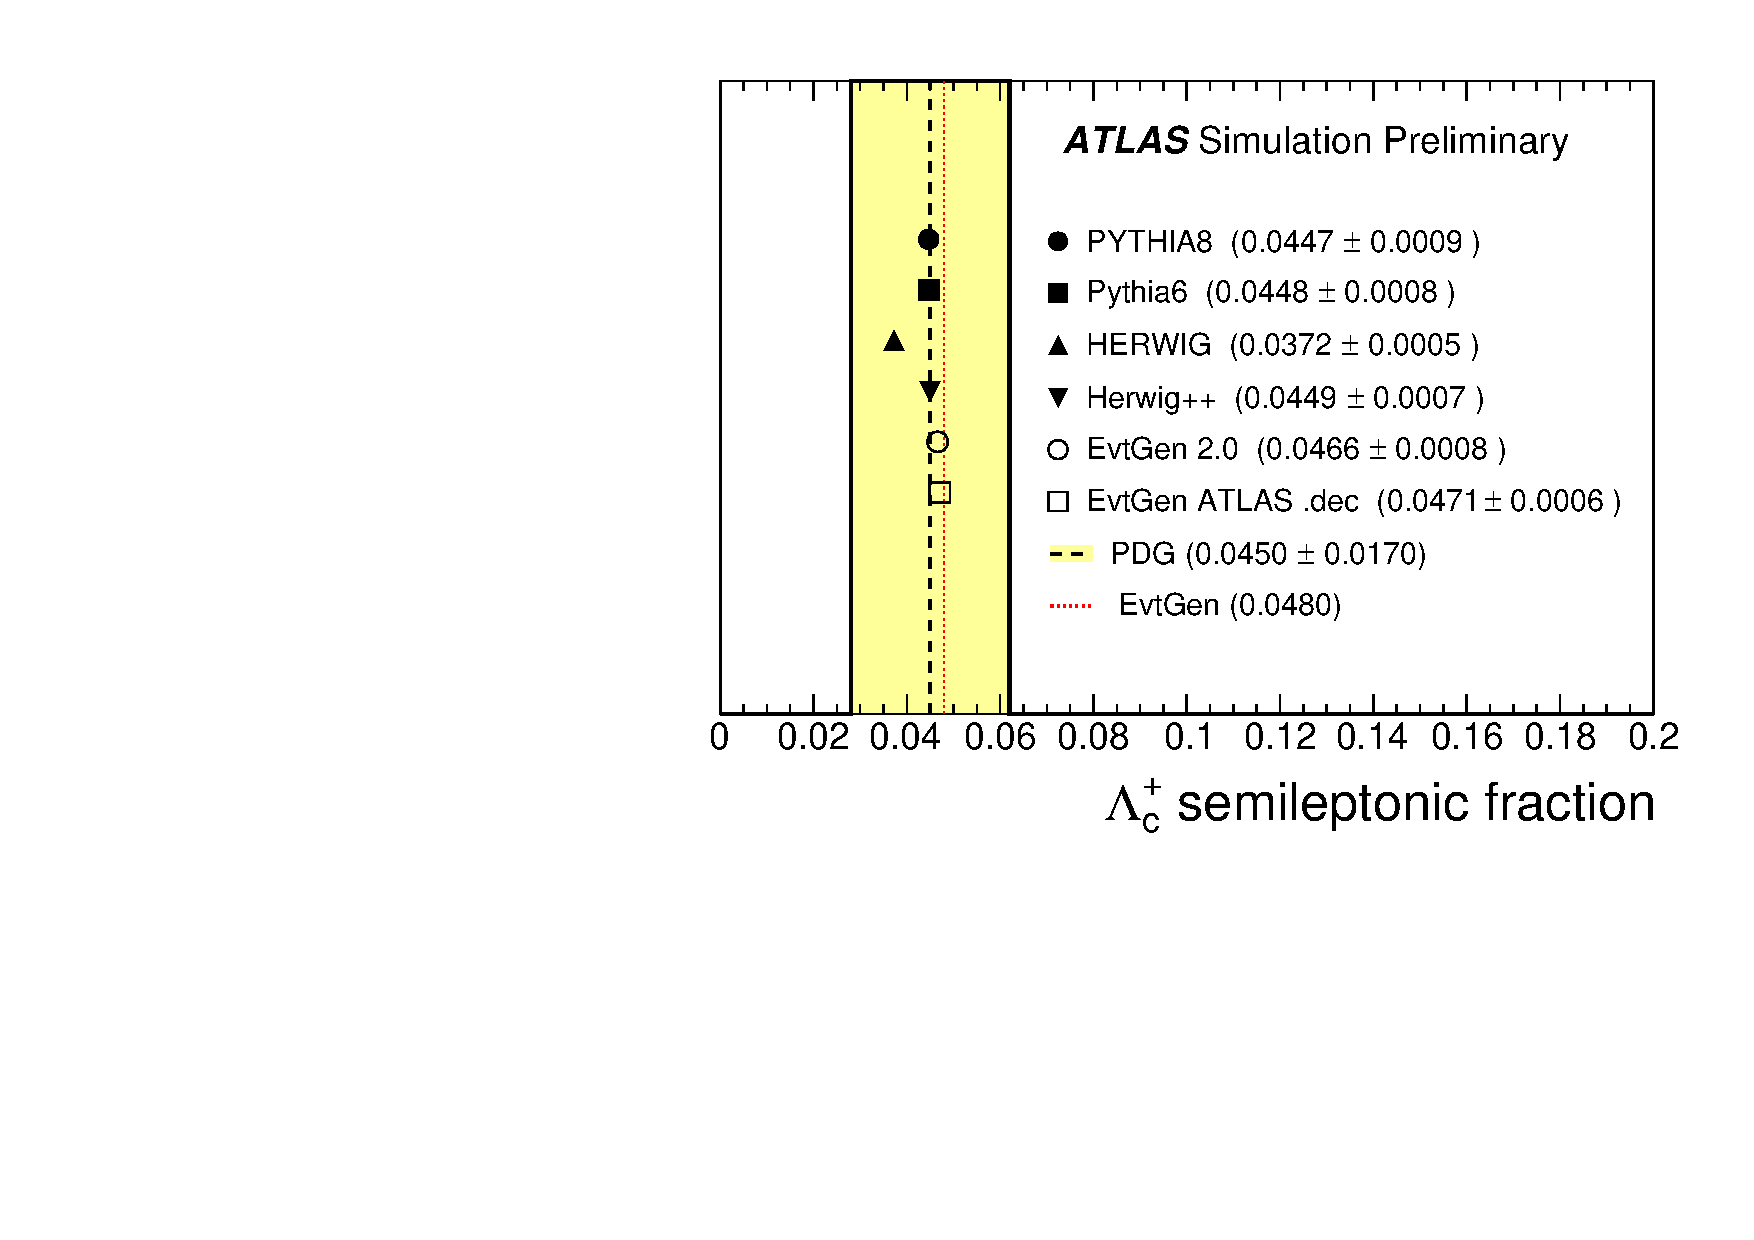
\includegraphics[width=\textwidth]{evtgen/figures/EvtGen/h_Lambdac_sl.pdf}
\end{subfigure}
\caption{Comparison of semileptonic branching fraction $D\rightarrow e^-\overline{\nu_e} X$
of the weakly decaying charm hadrons 
(a) \Dzero, (b) \Dplus, (c) \Ds\ and (d) \Lc~
in four different generators,
\Pythia\ version 427.2, \PythiaE\ version 175, \Herwigpp\  version 2.6.3 and \Herwig\ version 6.520.2, 
both with and without
\EvtGen.  
\EvtGen\ version 2.0 is used with the particle properties table provided with \EvtGen\ and with 
its standard inclusive decay table DECAY\_2010.DEC, as well as a custom decay table with developed for ATLAS with the most up to date semileptonic fractions from the PDG.
Only decays where the electron is the direct decay product of the charm are included.
The values of the $D^0$, $D^+$, $D^+_s$ and $\Lambda^+_c$~semileptonic fractions in this default 
\EvtGen\  particle properties table differ from the world averages listed by the PDG~\cite{PhysRevD.86.010001}.}
\label{fig:csl}
\end{figure}
\begin{figure}
\centering
\begin{subfigure}[]{0.45\textwidth}
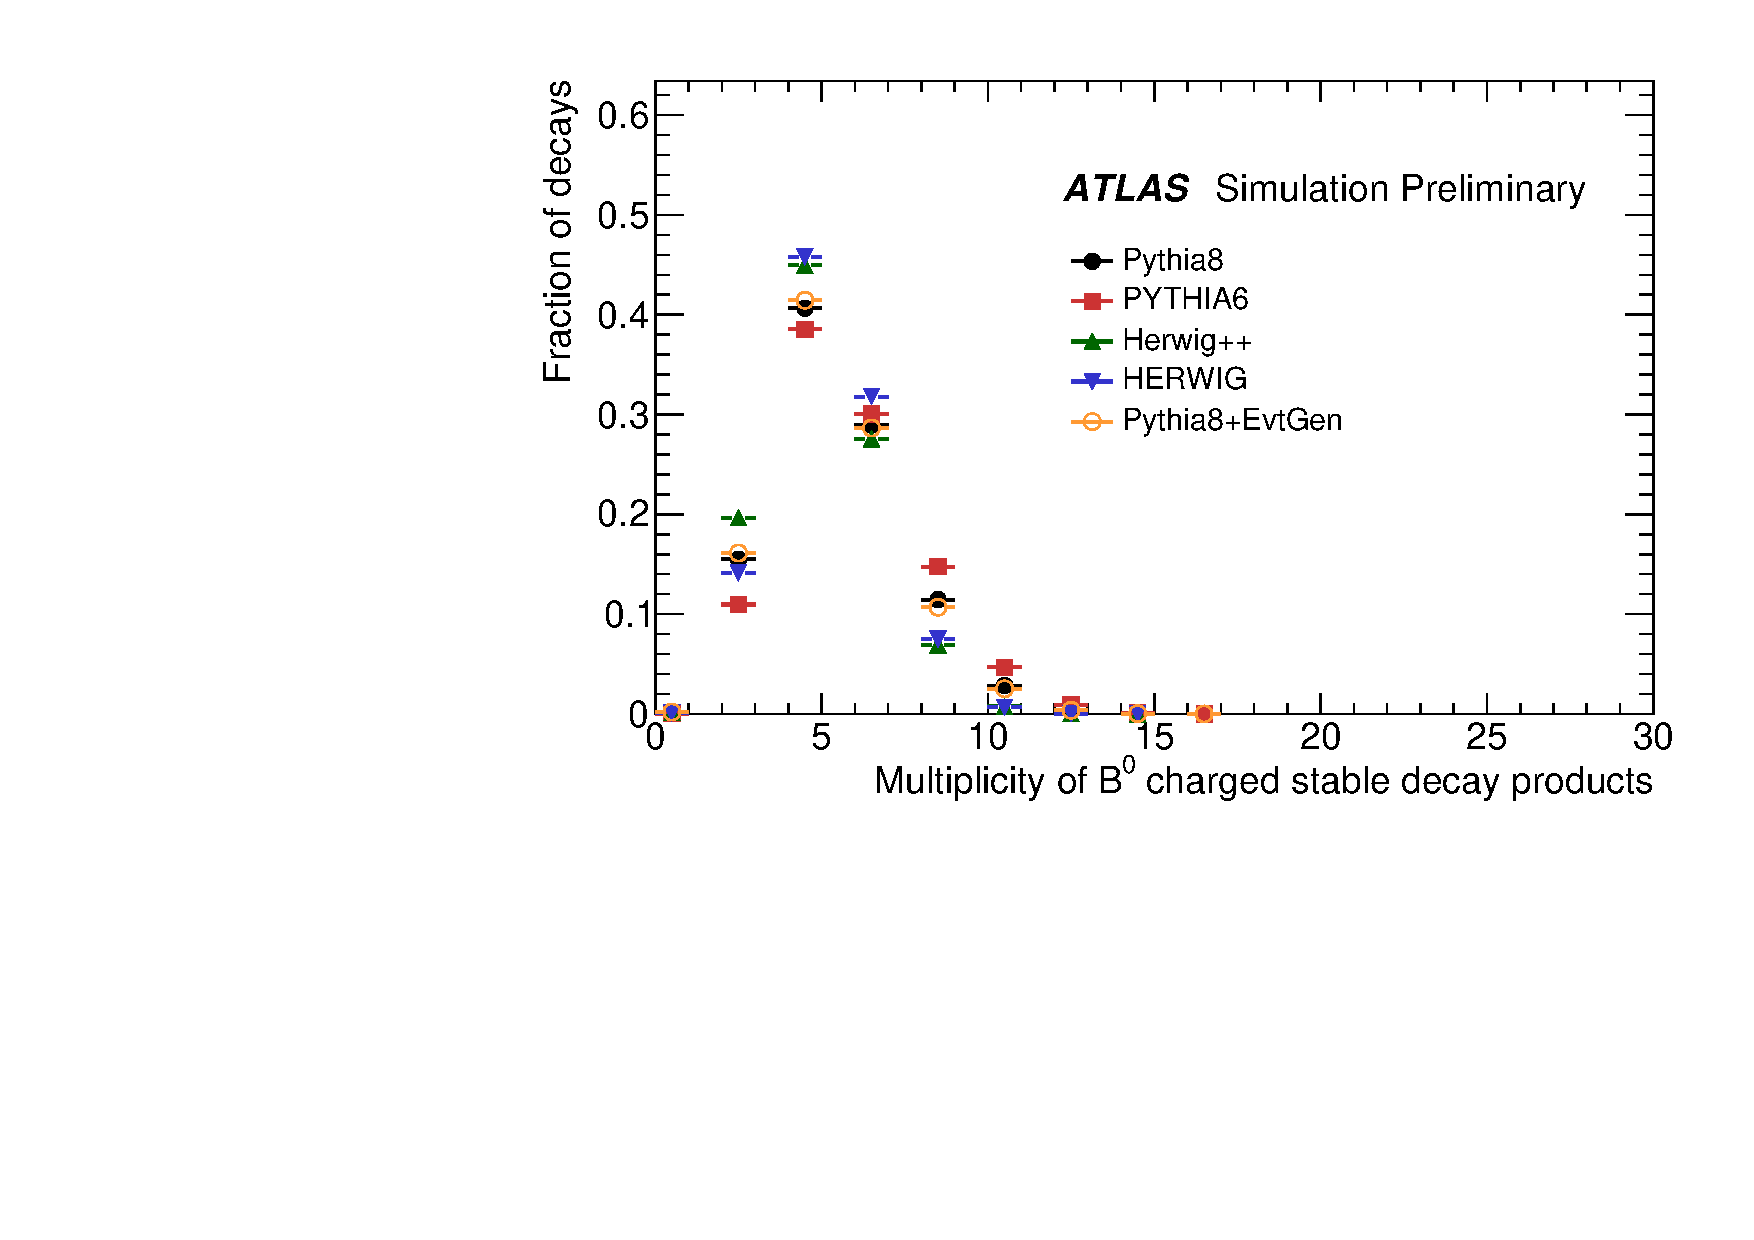
\includegraphics[width=\textwidth]{evtgen/figures/EvtGen/B0/h_species_ncharge.pdf}
\end{subfigure}
\begin{subfigure}[]{0.45\textwidth}
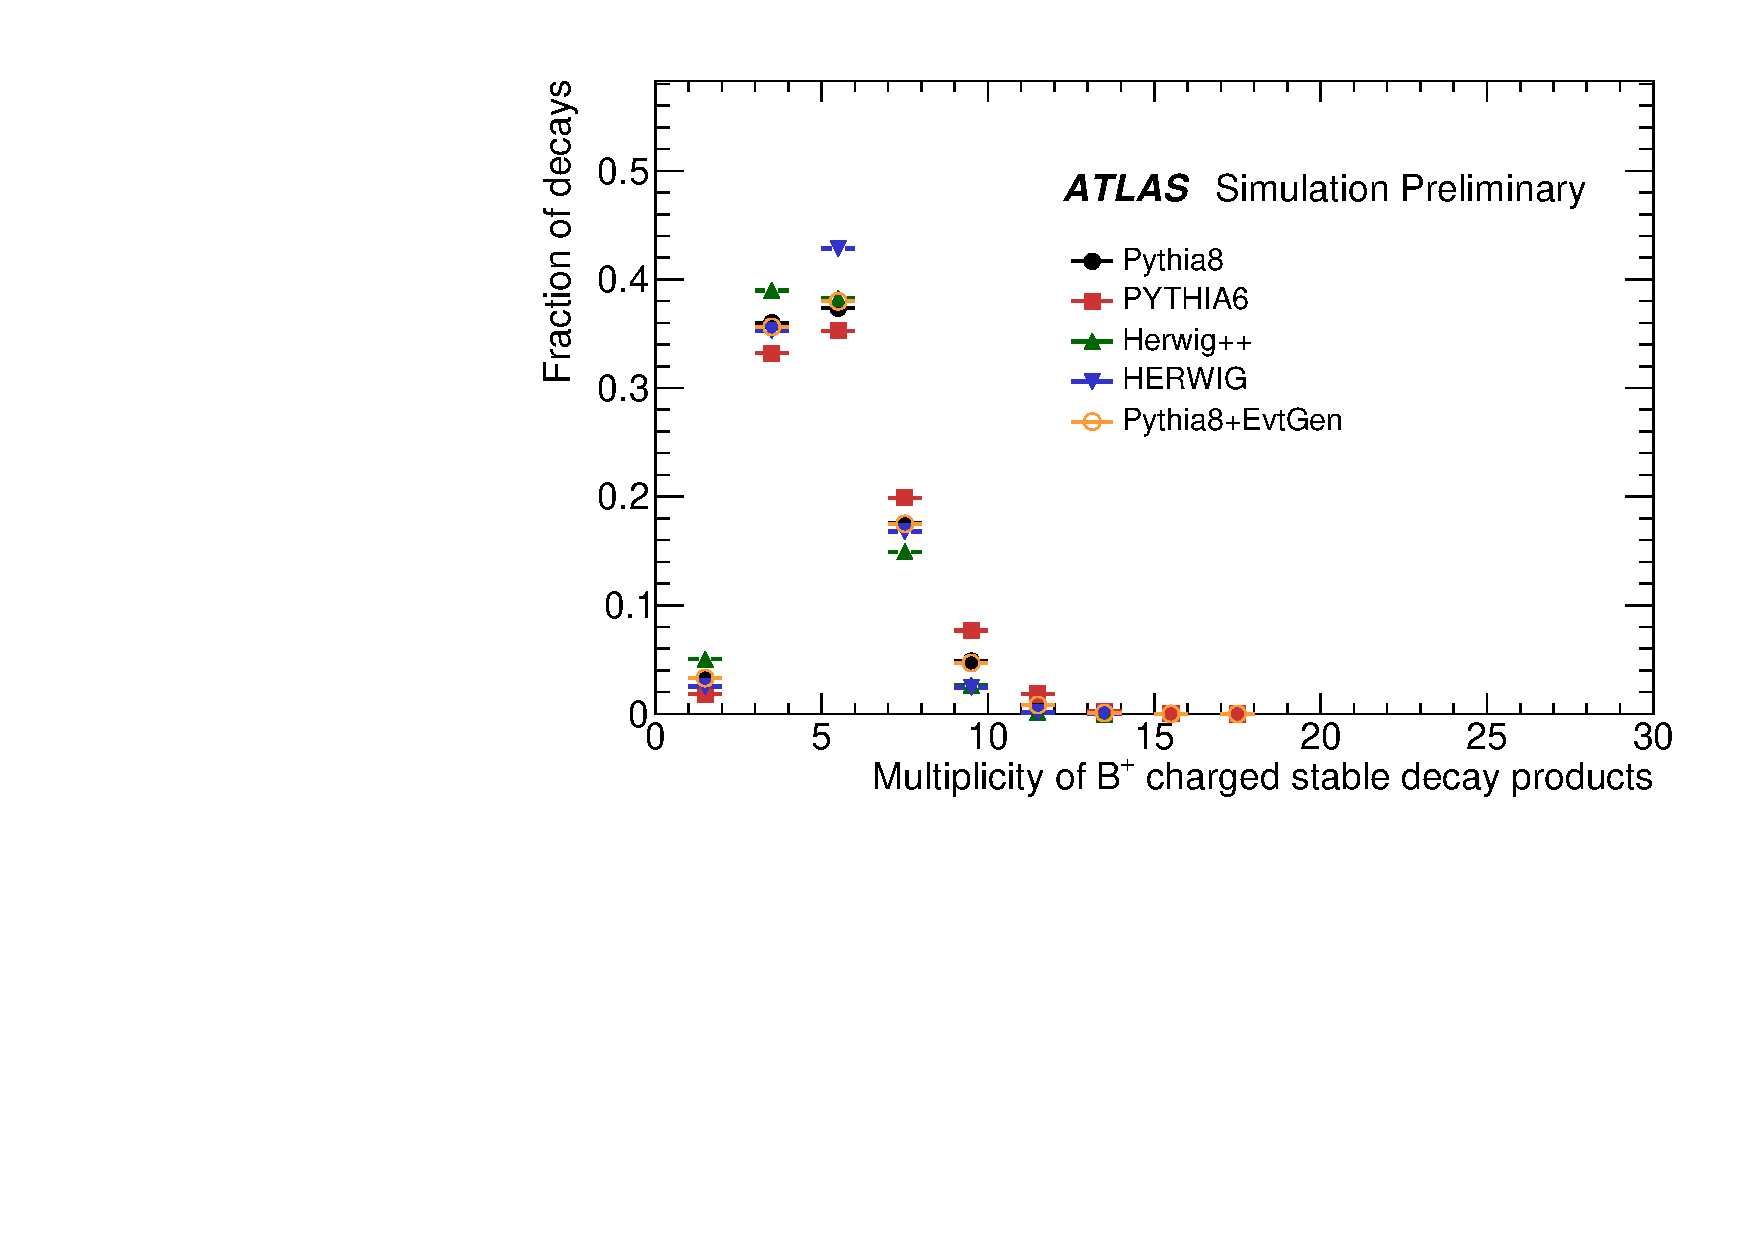
\includegraphics[width=\textwidth]{evtgen/figures/EvtGen/B+/h_species_ncharge.pdf}
\end{subfigure}\\
\begin{subfigure}[]{0.45\textwidth}
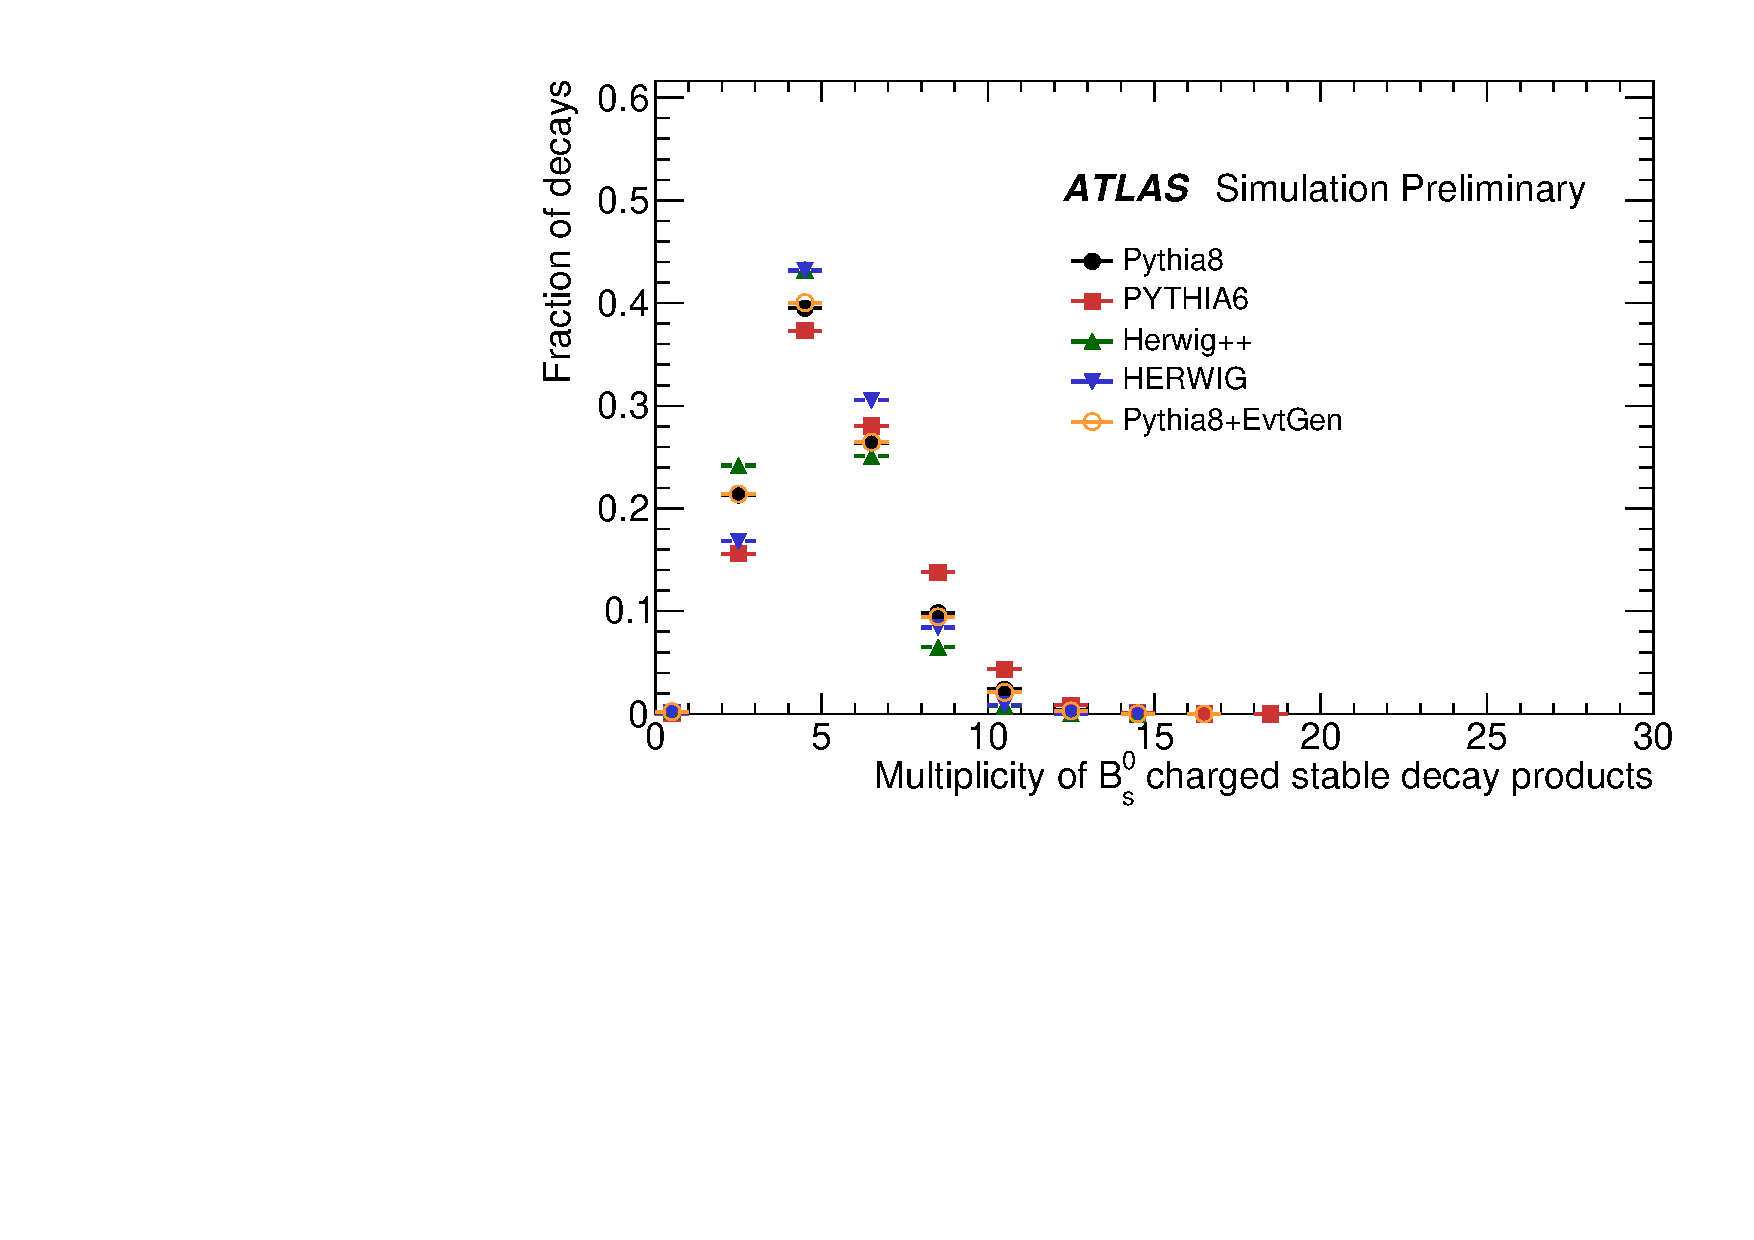
\includegraphics[width=\textwidth]{evtgen/figures/EvtGen/Bs0/h_species_ncharge.pdf}
\end{subfigure}
\begin{subfigure}[]{0.45\textwidth}
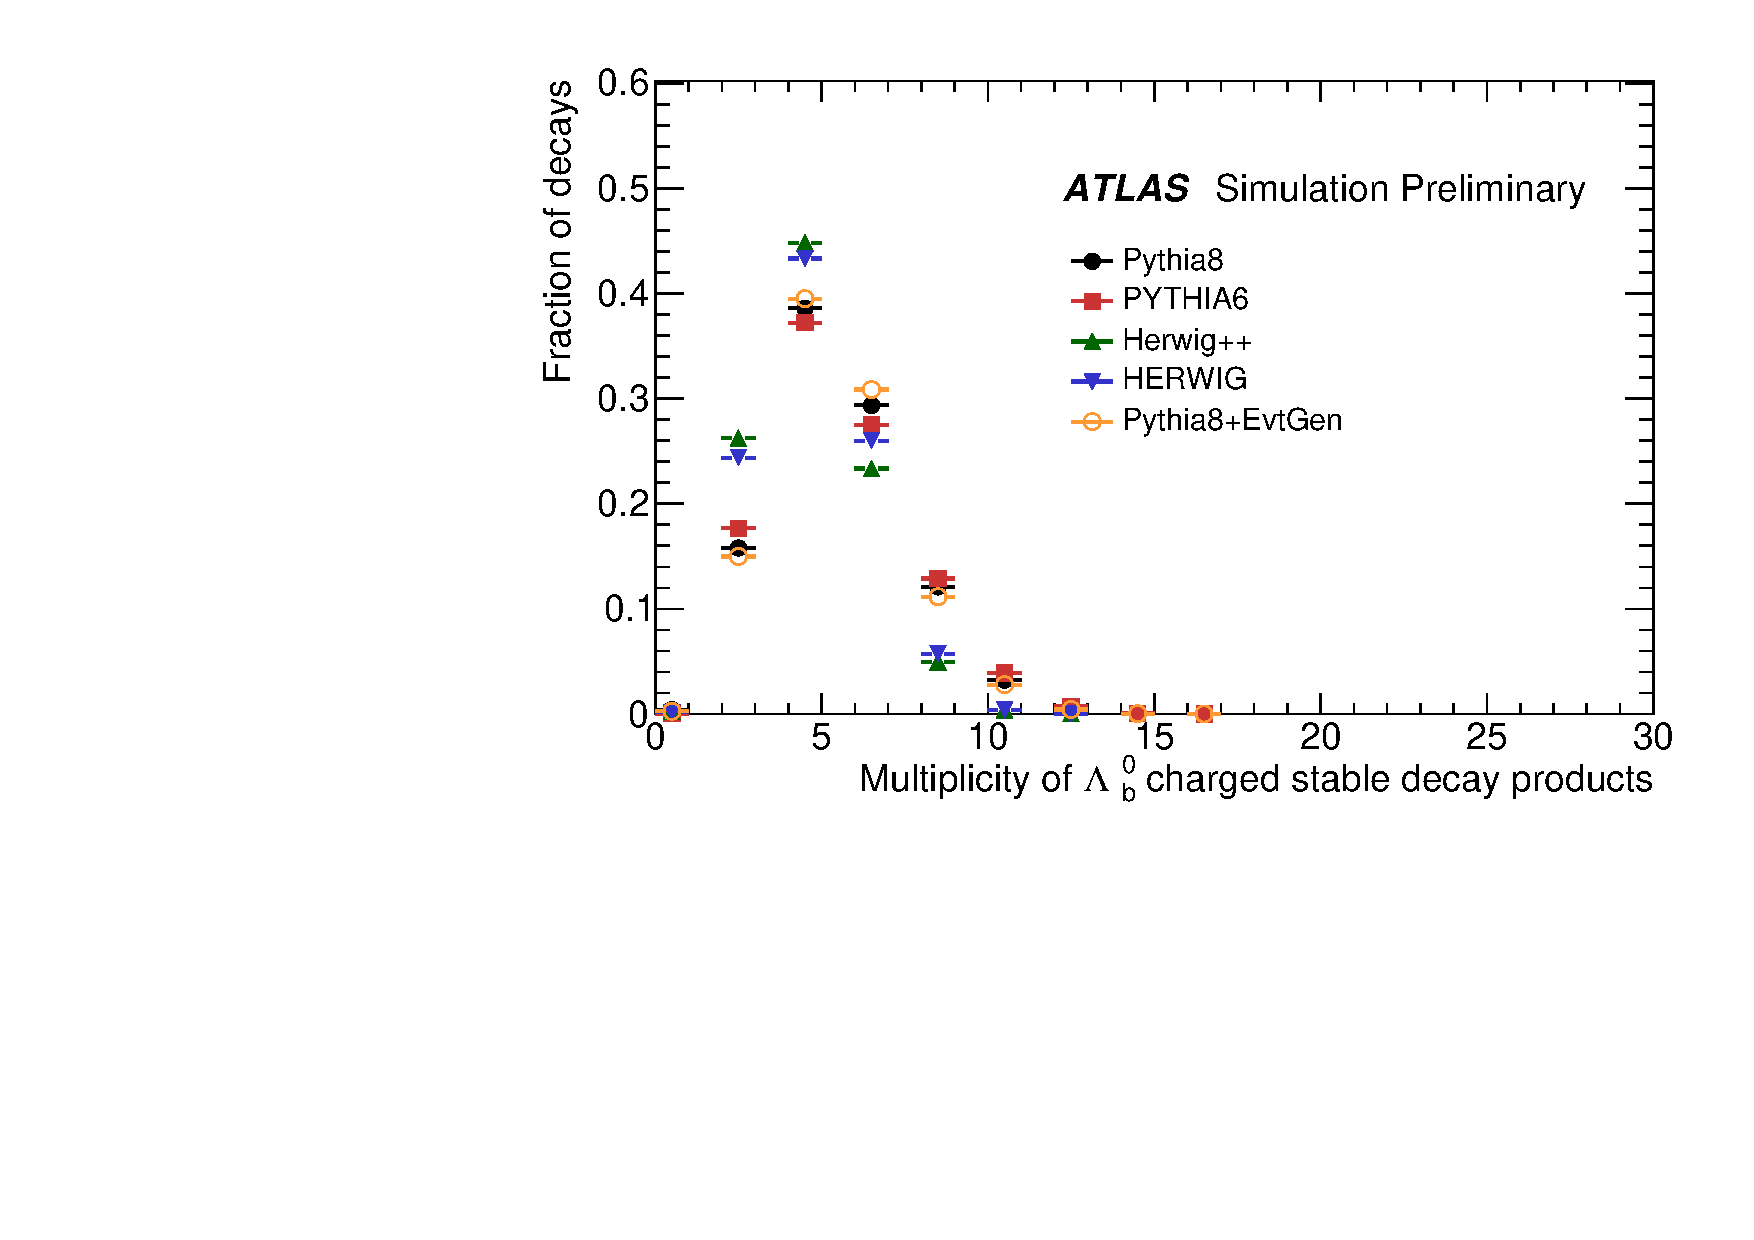
\includegraphics[width=\textwidth]{evtgen/figures/EvtGen/Lambdab0/h_species_ncharge.pdf}
\end{subfigure}
\caption{Comparison of the multiplicity of charged, stable decay products for the weakly decaying bottom hadrons 
(a) $B_0$, (b) $B^{+}$, (c) \Bs~ and (d) \Lb~
in \PythiaE\,~ \Pythia\,~ \newline \Herwigpp\, \Herwig\ and \EvtGen. A stable particle is defined
as a particle with a proper lifetime $c\tau_{0}>10$~mm. }
\label{fig:bcharge}
\end{figure}

\begin{figure}
\centering
\begin{subfigure}[]{0.45\textwidth}
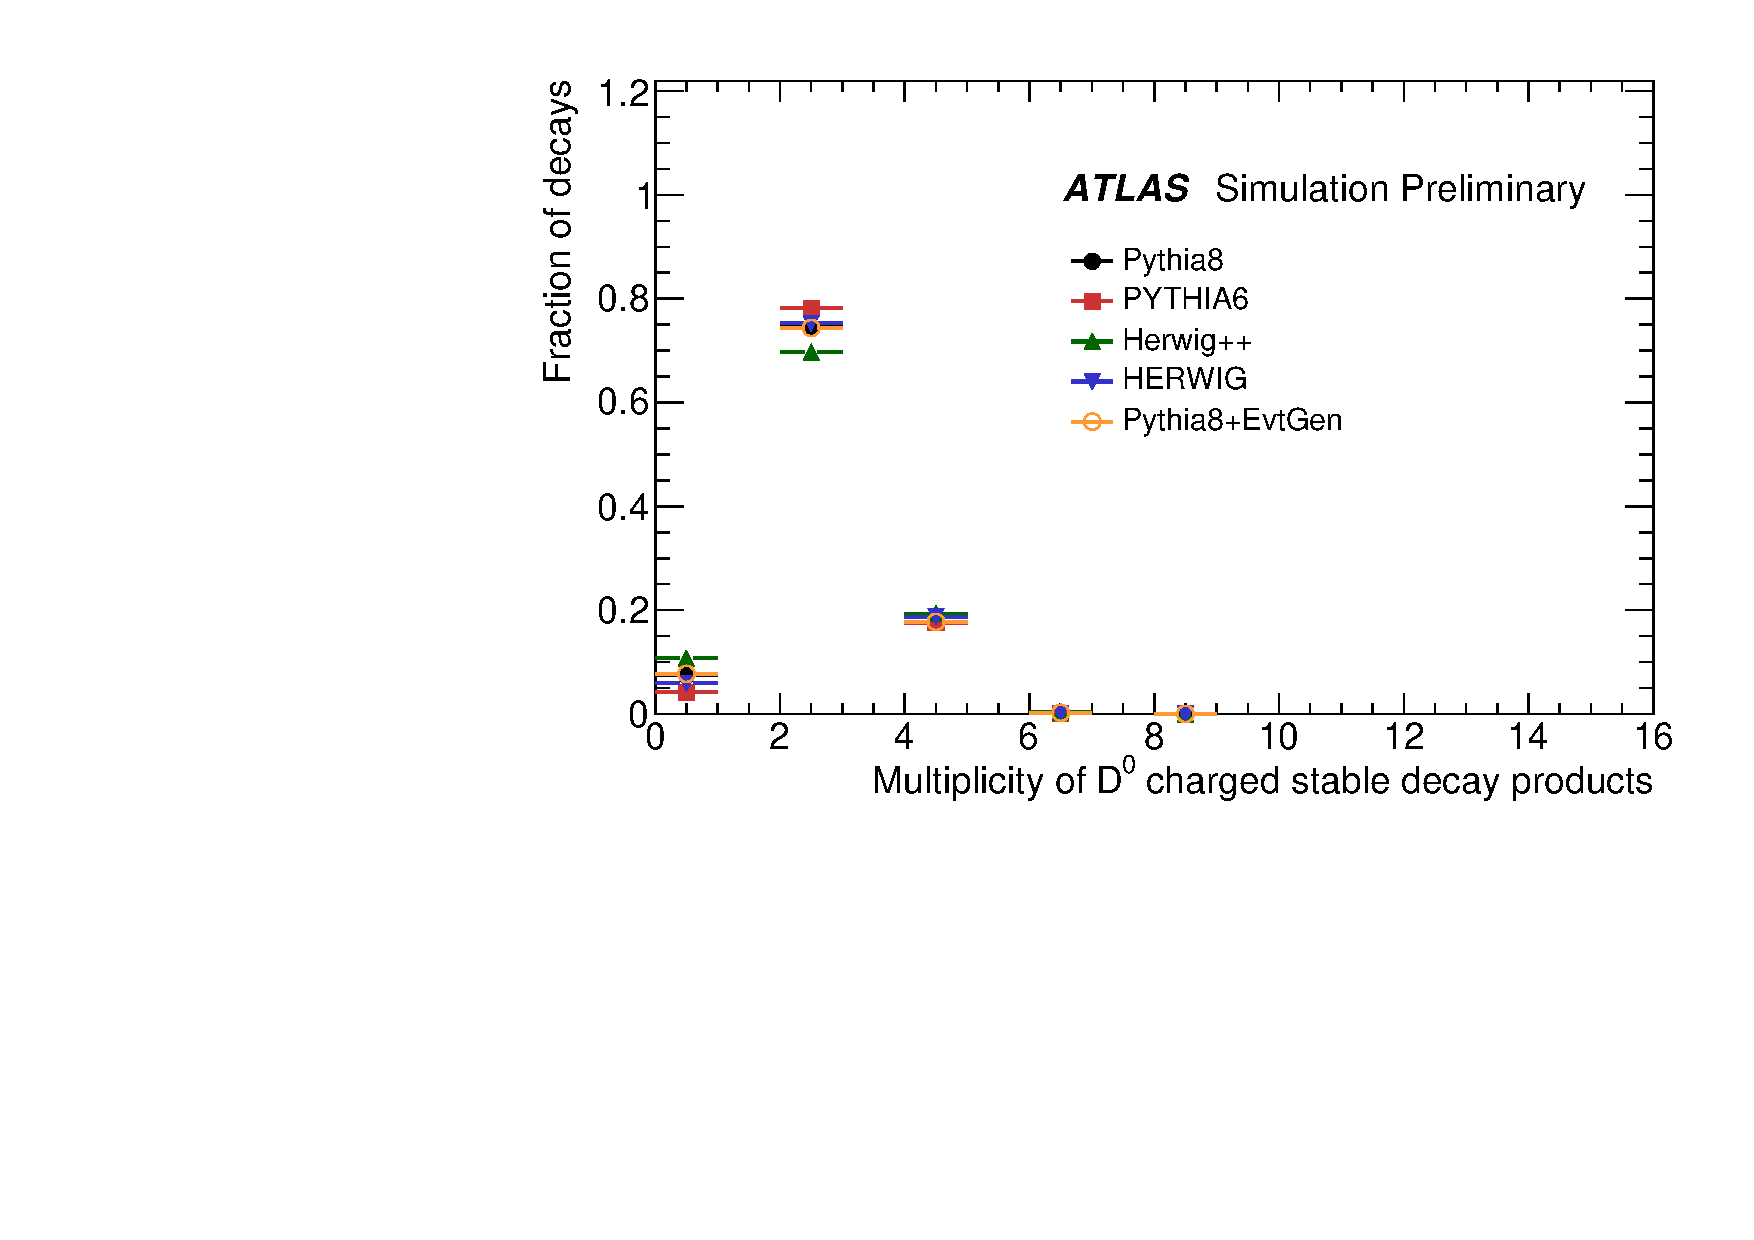
\includegraphics[width=\textwidth]{evtgen/figures/EvtGen/D0/h_species_ncharge.pdf}
\end{subfigure}
\begin{subfigure}[]{0.45\textwidth}
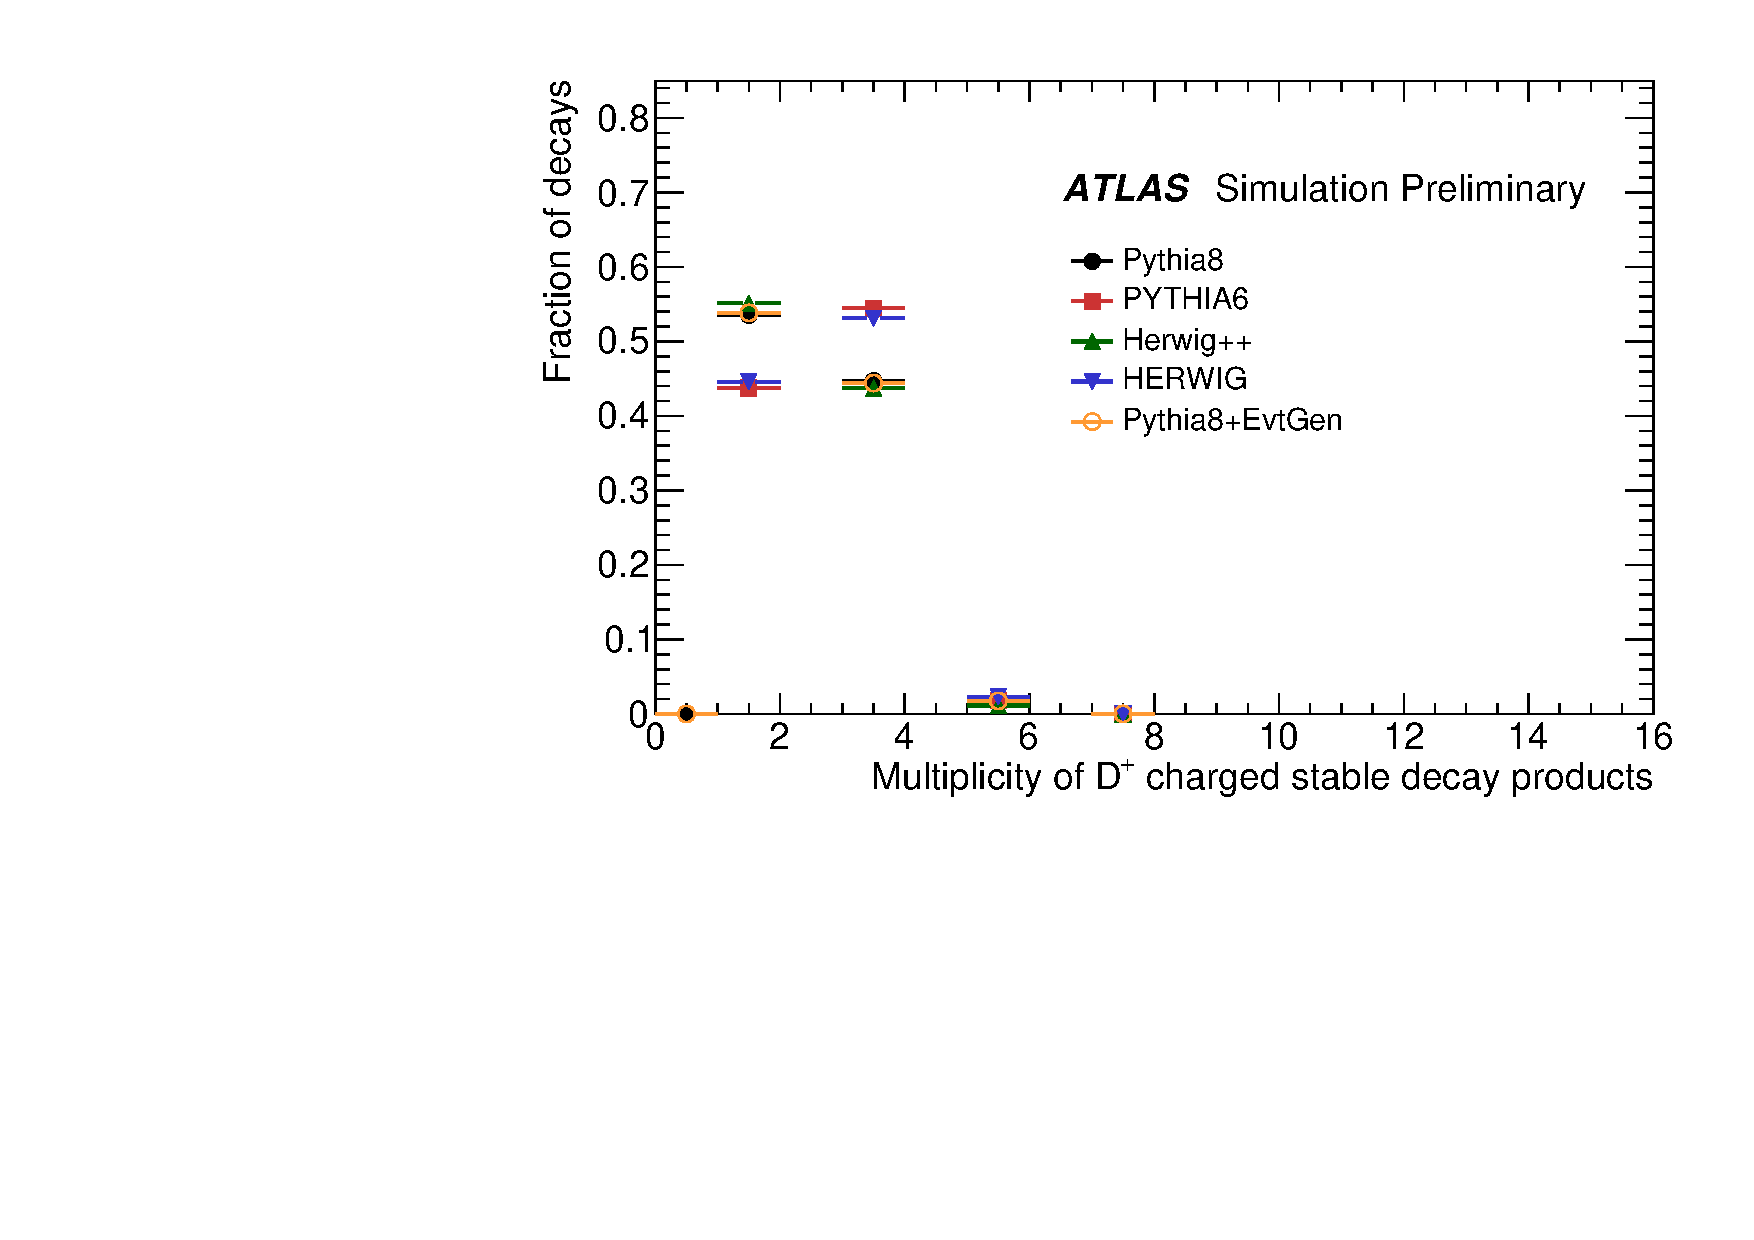
\includegraphics[width=\textwidth]{evtgen/figures/EvtGen/D+/h_species_ncharge.pdf}
\end{subfigure}\\
\begin{subfigure}[]{0.45\textwidth}
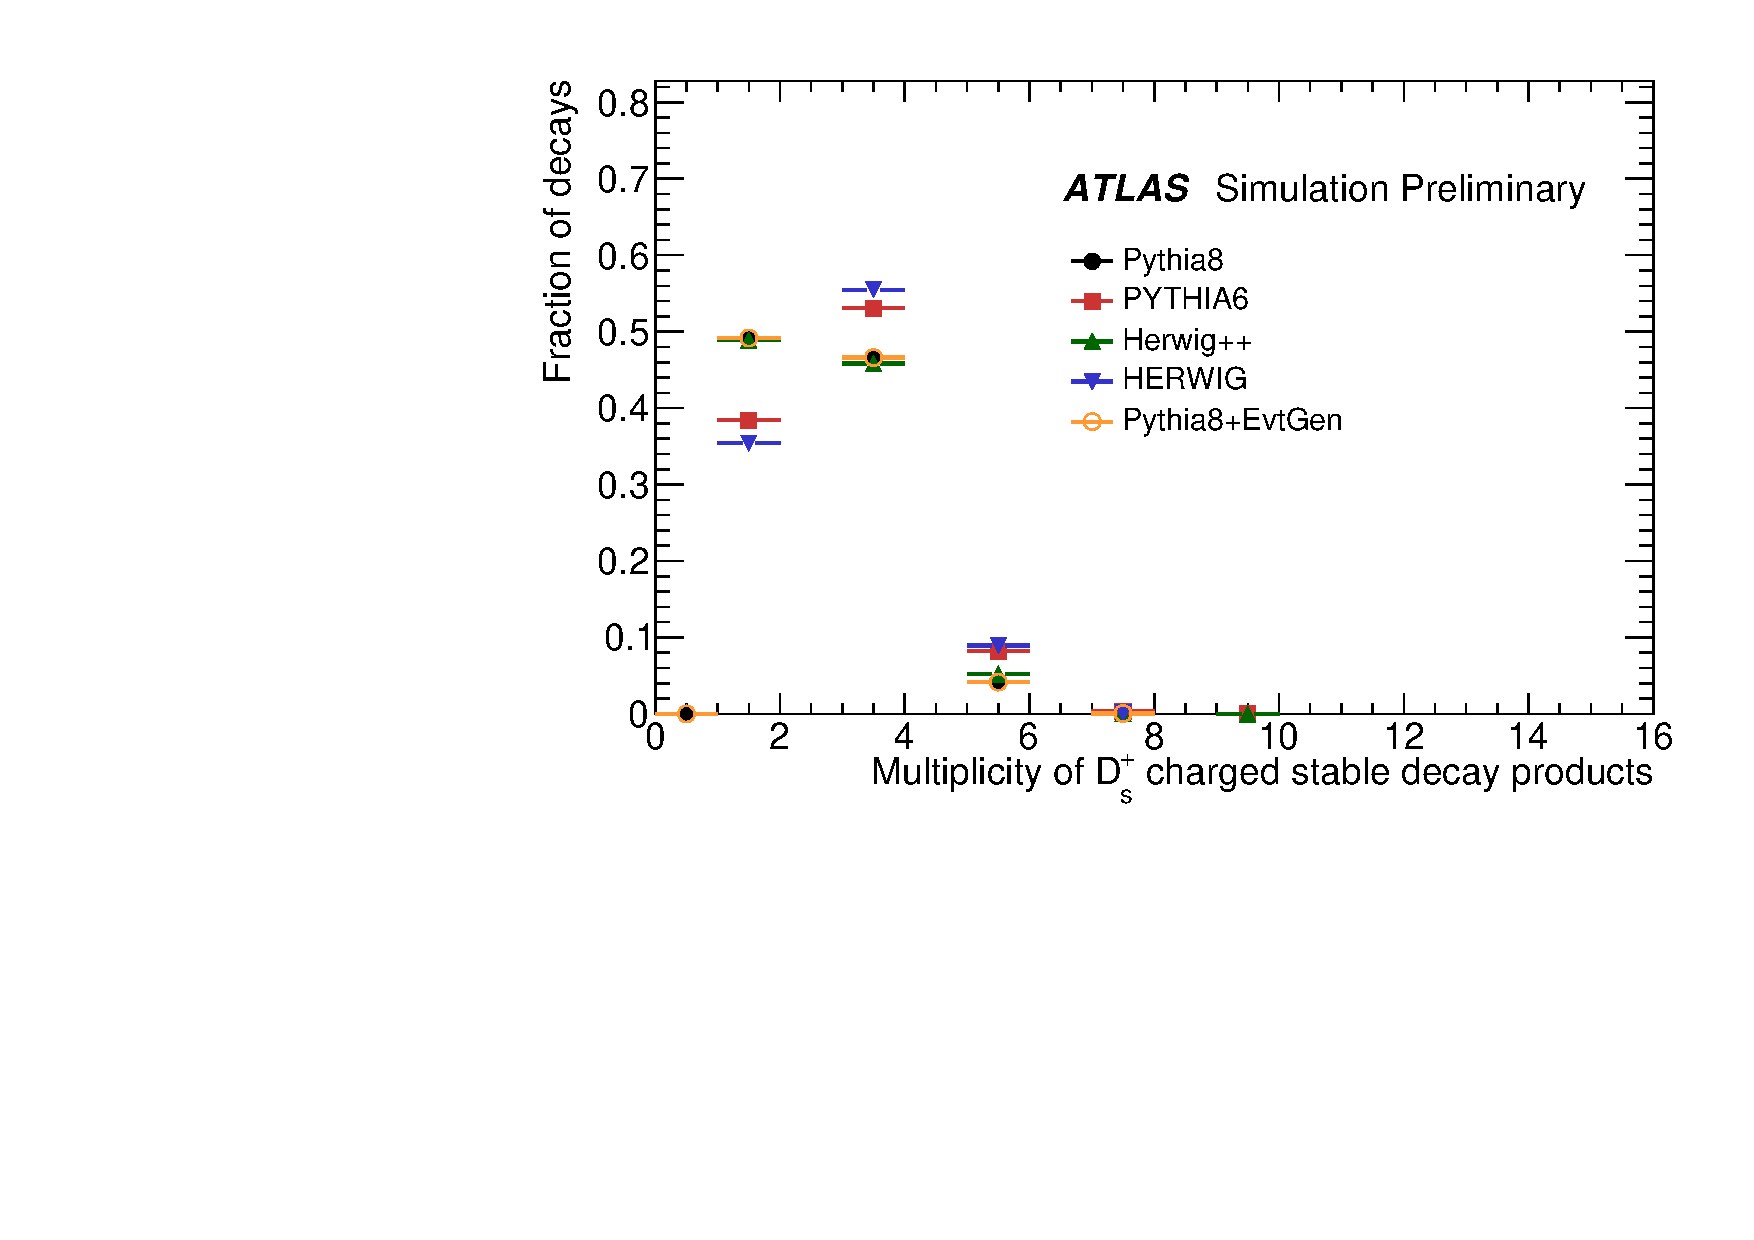
\includegraphics[width=\textwidth]{evtgen/figures/EvtGen/Ds+/h_species_ncharge.pdf}
\end{subfigure}
\begin{subfigure}[]{0.45\textwidth}
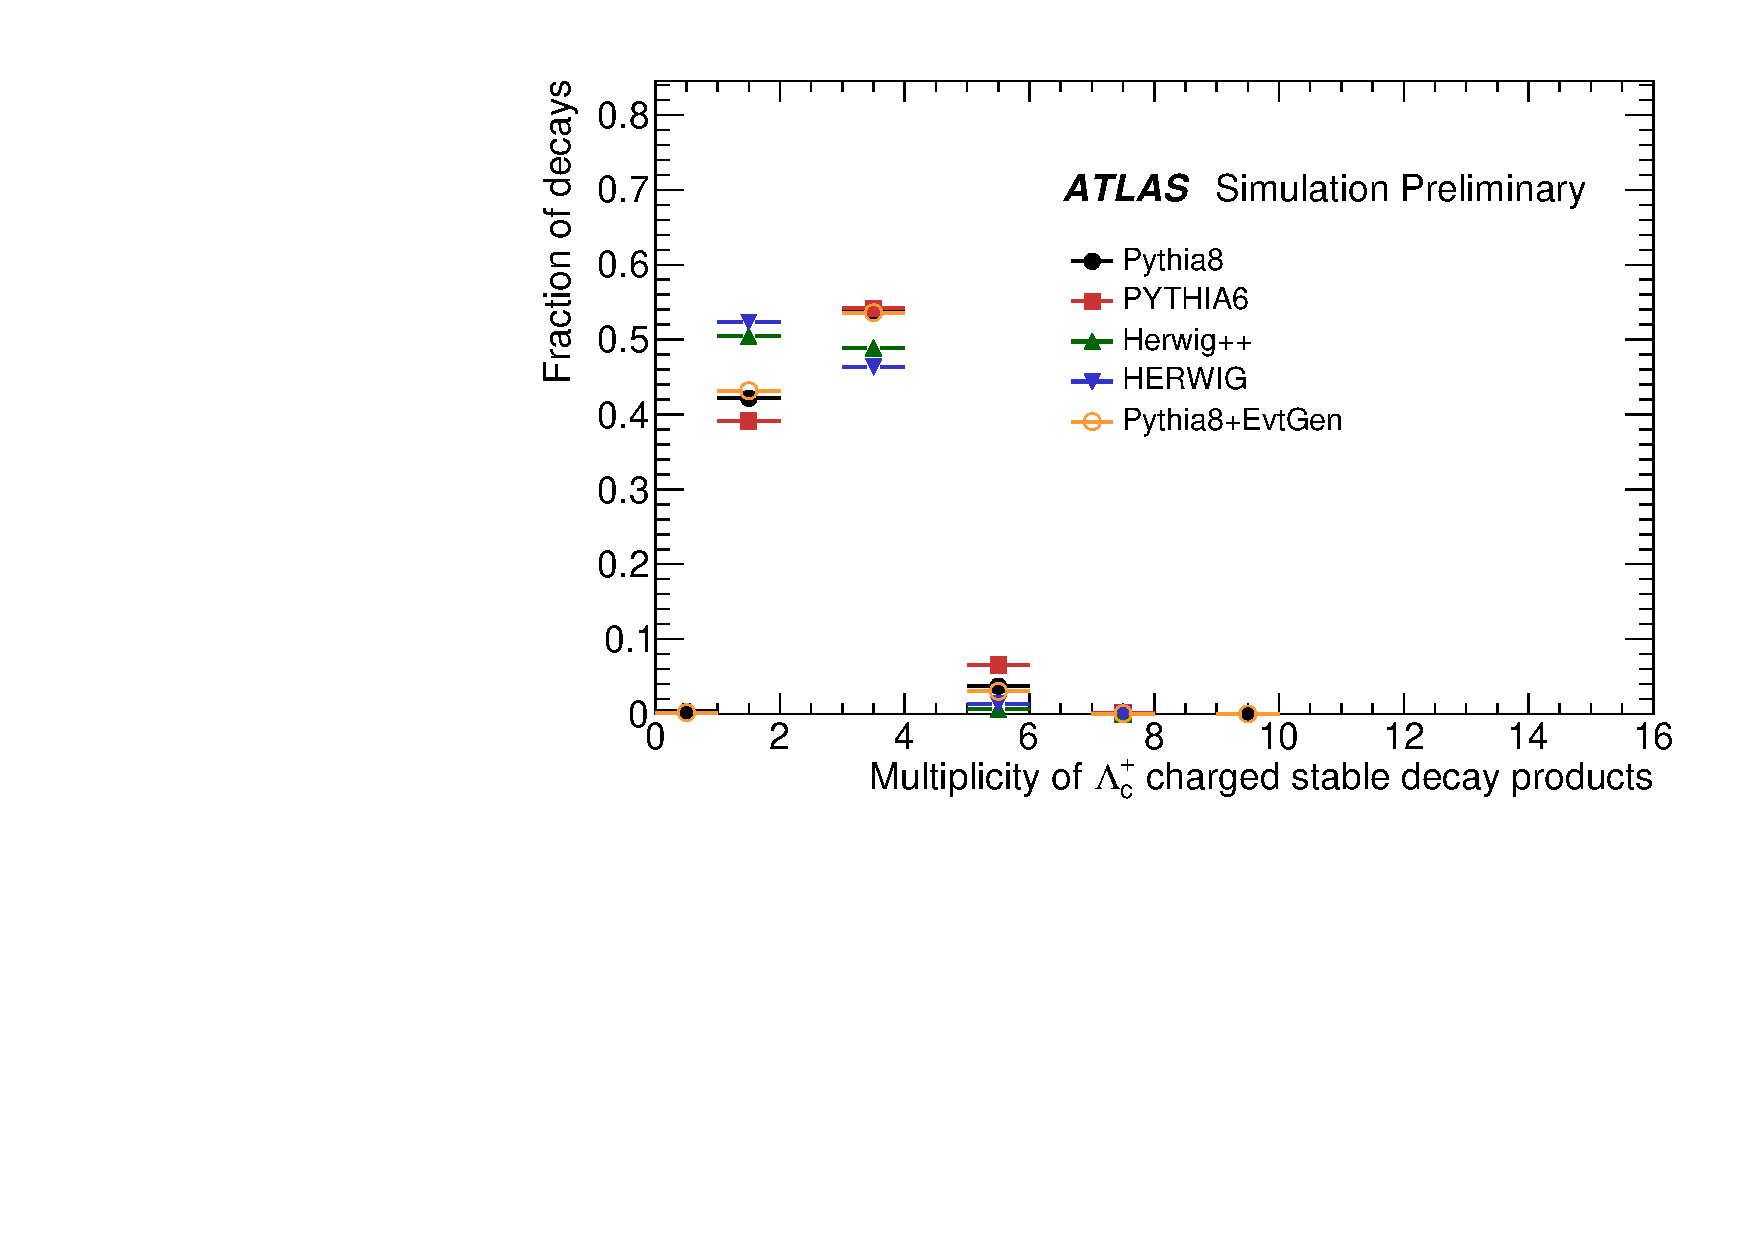
\includegraphics[width=\textwidth]{evtgen/figures/EvtGen/Lambdac+/h_species_ncharge.pdf}
\end{subfigure}
\caption{Comparison of multiplicity of charged, stable decay products for the weakly decaying 
charm hadrons 
(a) \Dzero,~ (b) \Dplus,~ (c) \Ds\ and (d) \Lc~
in \PythiaE\,~ \Pythia\, \newline  \Herwigpp\, ~\Herwig\ and \EvtGen.  A stable particle is defined
as a particle with a proper lifetime $c\tau_{0}>10$~mm. } 
\label{fig:ccharge}
\end{figure}

\begin{figure}
\centering
\begin{subfigure}[]{0.45\textwidth}
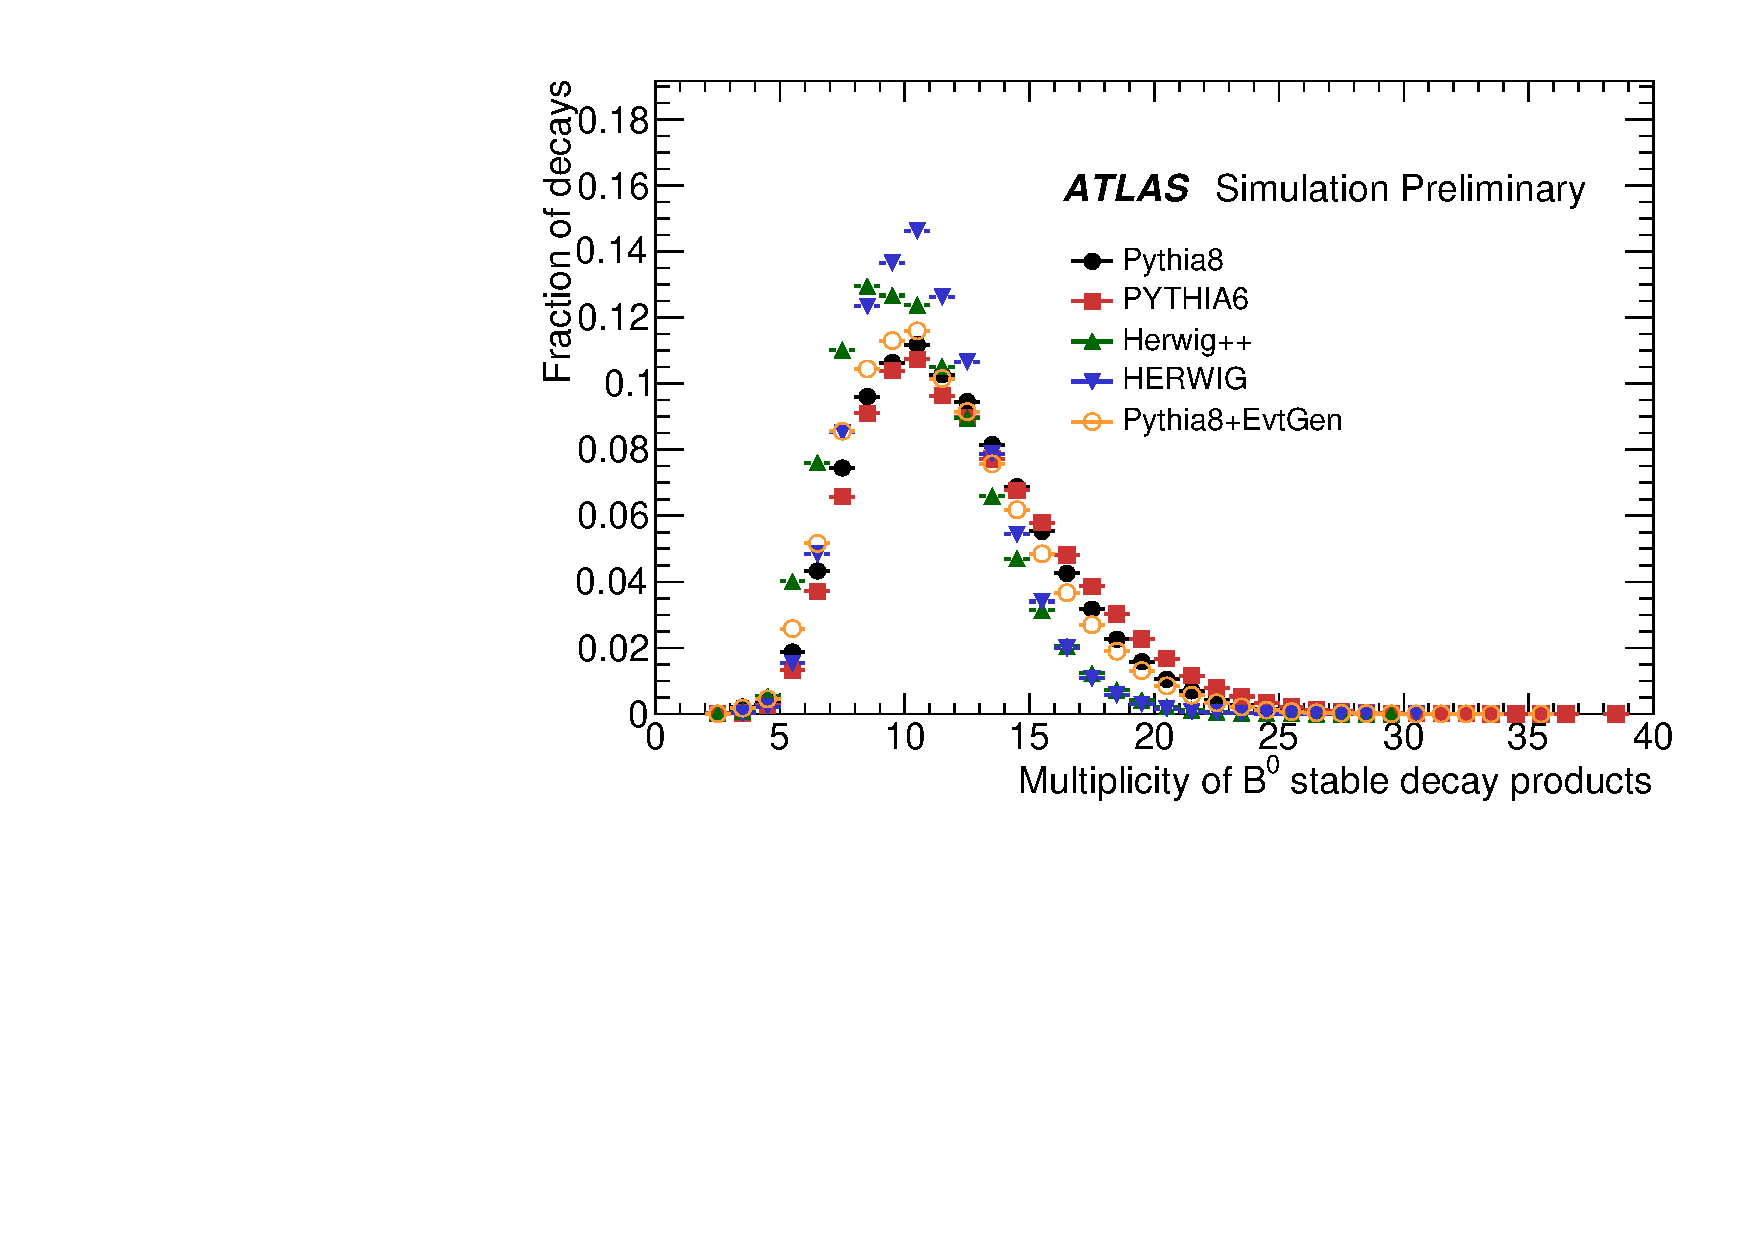
\includegraphics[width=\textwidth]{evtgen/figures/EvtGen/B0/h_species_multiplicity.pdf}
\end{subfigure}
\begin{subfigure}[]{0.45\textwidth}
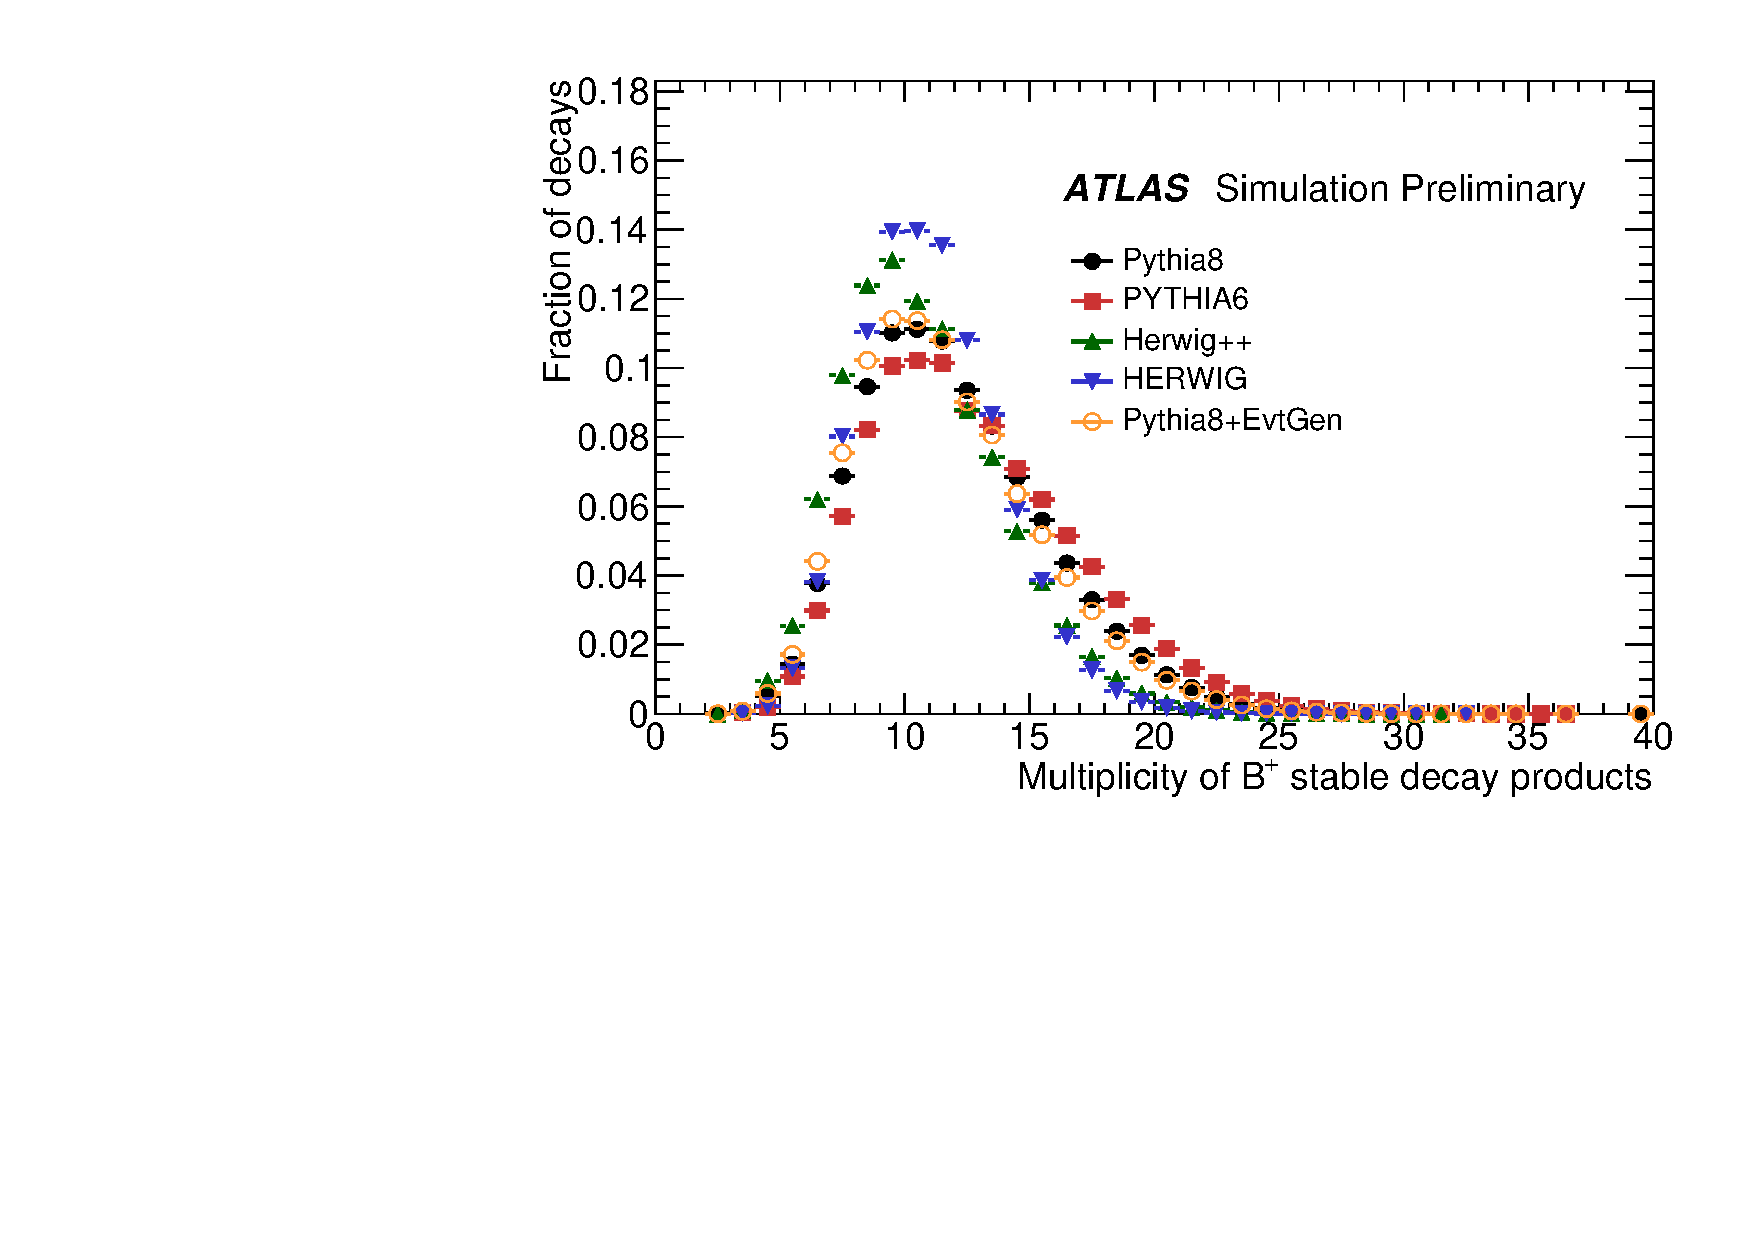
\includegraphics[width=\textwidth]{evtgen/figures/EvtGen/B+/h_species_multiplicity.pdf}
\end{subfigure}\\
\begin{subfigure}[]{0.45\textwidth}
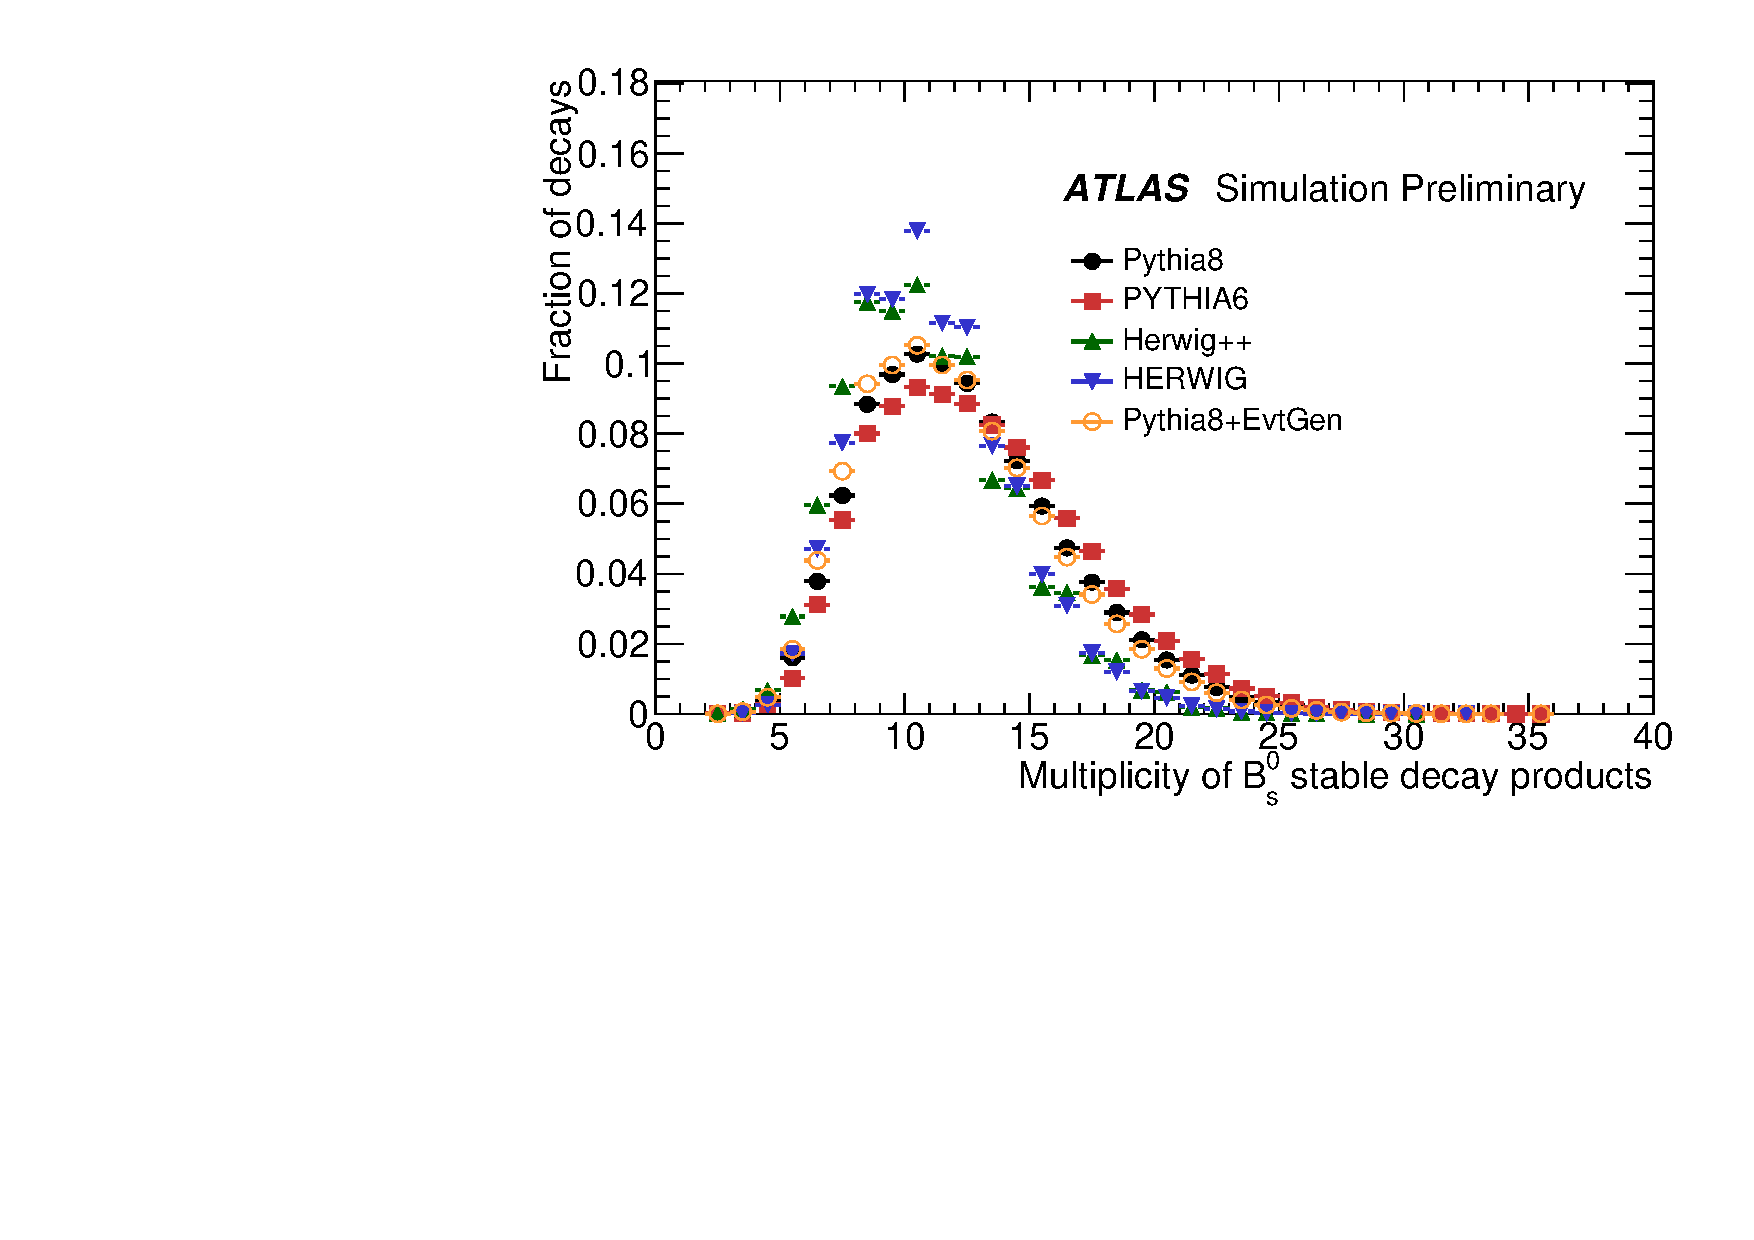
\includegraphics[width=\textwidth]{evtgen/figures/EvtGen/Bs0/h_species_multiplicity.pdf}
\end{subfigure}
\begin{subfigure}[]{0.45\textwidth}
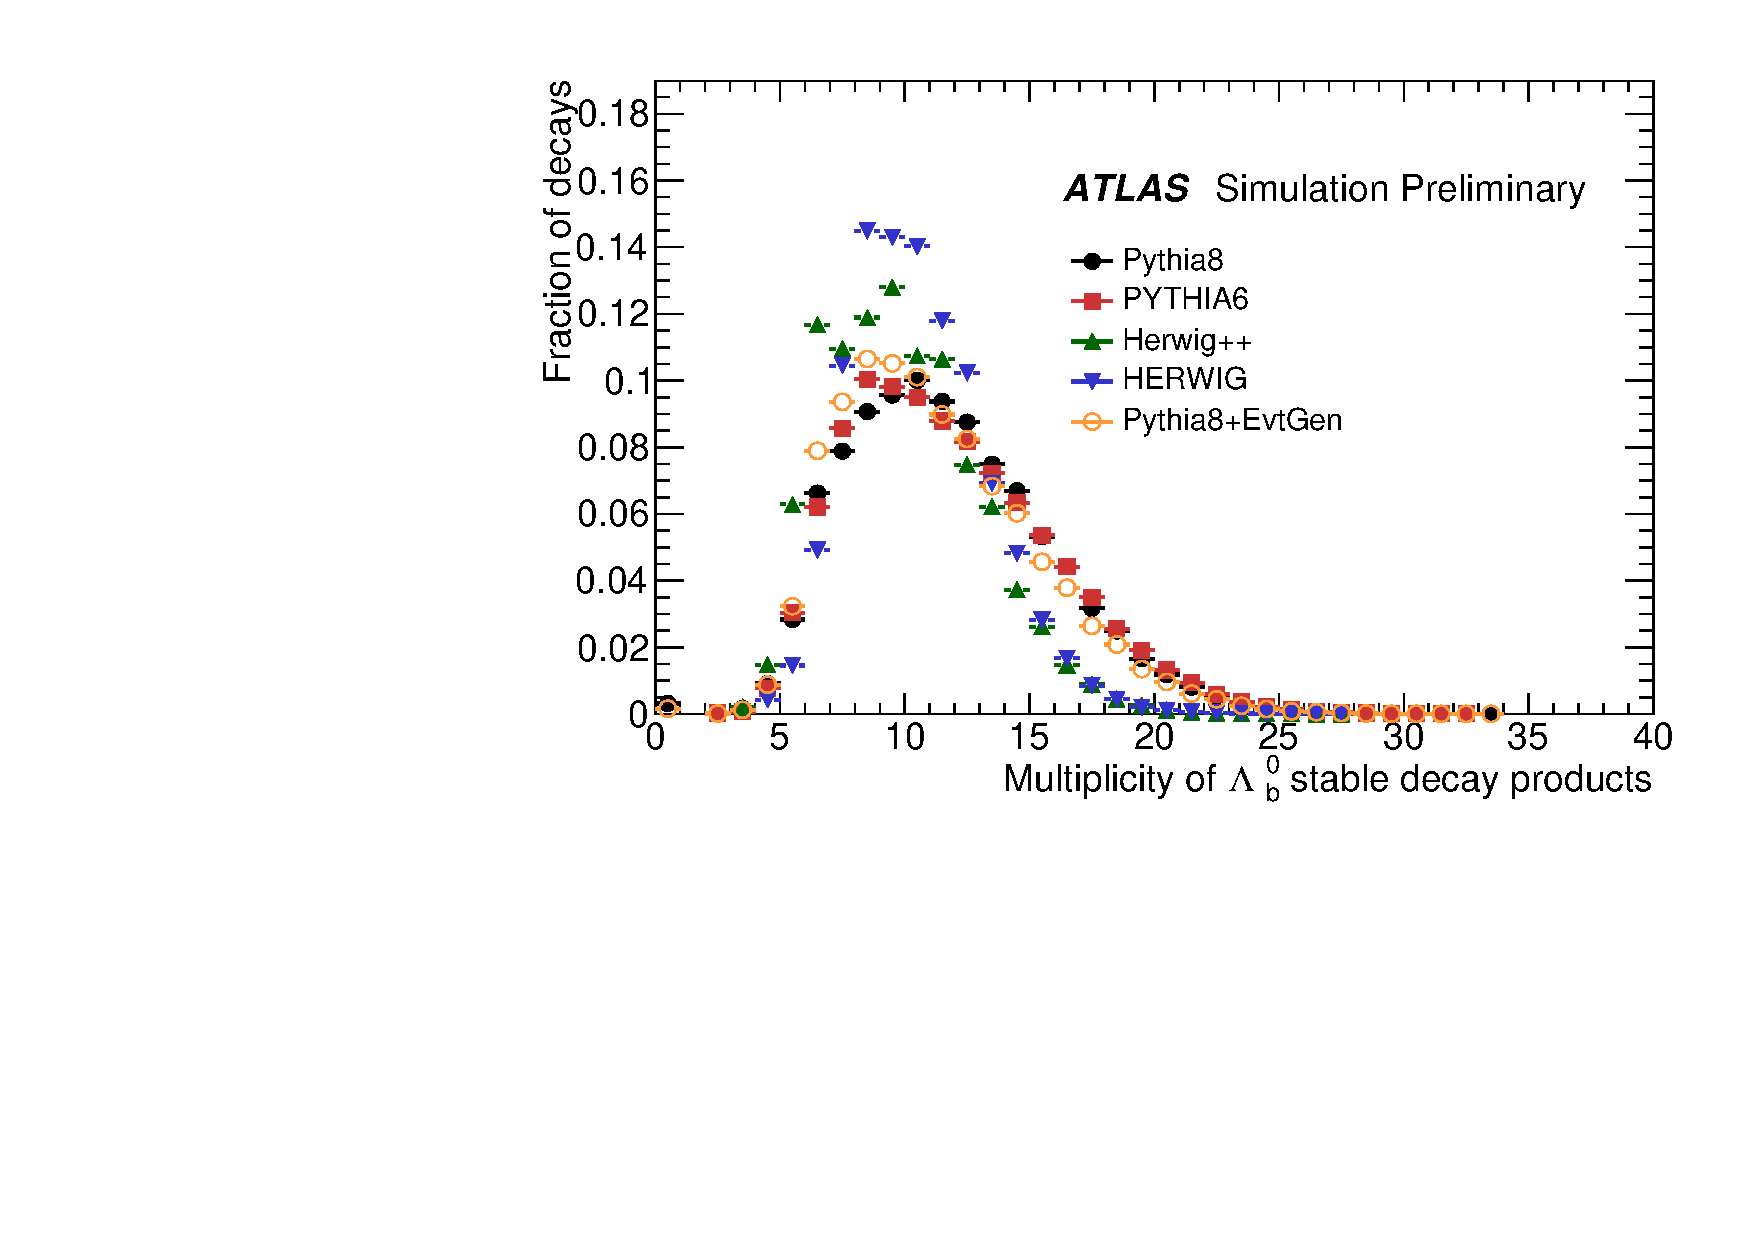
\includegraphics[width=\textwidth]{evtgen/figures/EvtGen/Lambdab0/h_species_multiplicity.pdf}
\end{subfigure}
\caption{Comparison of the multiplicity of stable decay products for the weakly decaying bottom hadrons 
(a) \Bo,~ (b) \Bp,~ (c) \Bs~ and (d) \Lb~
in \PythiaE\,~ \Pythia\, \newline  \Herwigpp\, ~\Herwig\ and \EvtGen.  A stable particle is defined
as a particle with a proper lifetime $c\tau_{0}>10$~mm. }
\label{fig:bmult}
\end{figure}

\begin{figure}
\centering
\begin{subfigure}[]{0.45\textwidth}
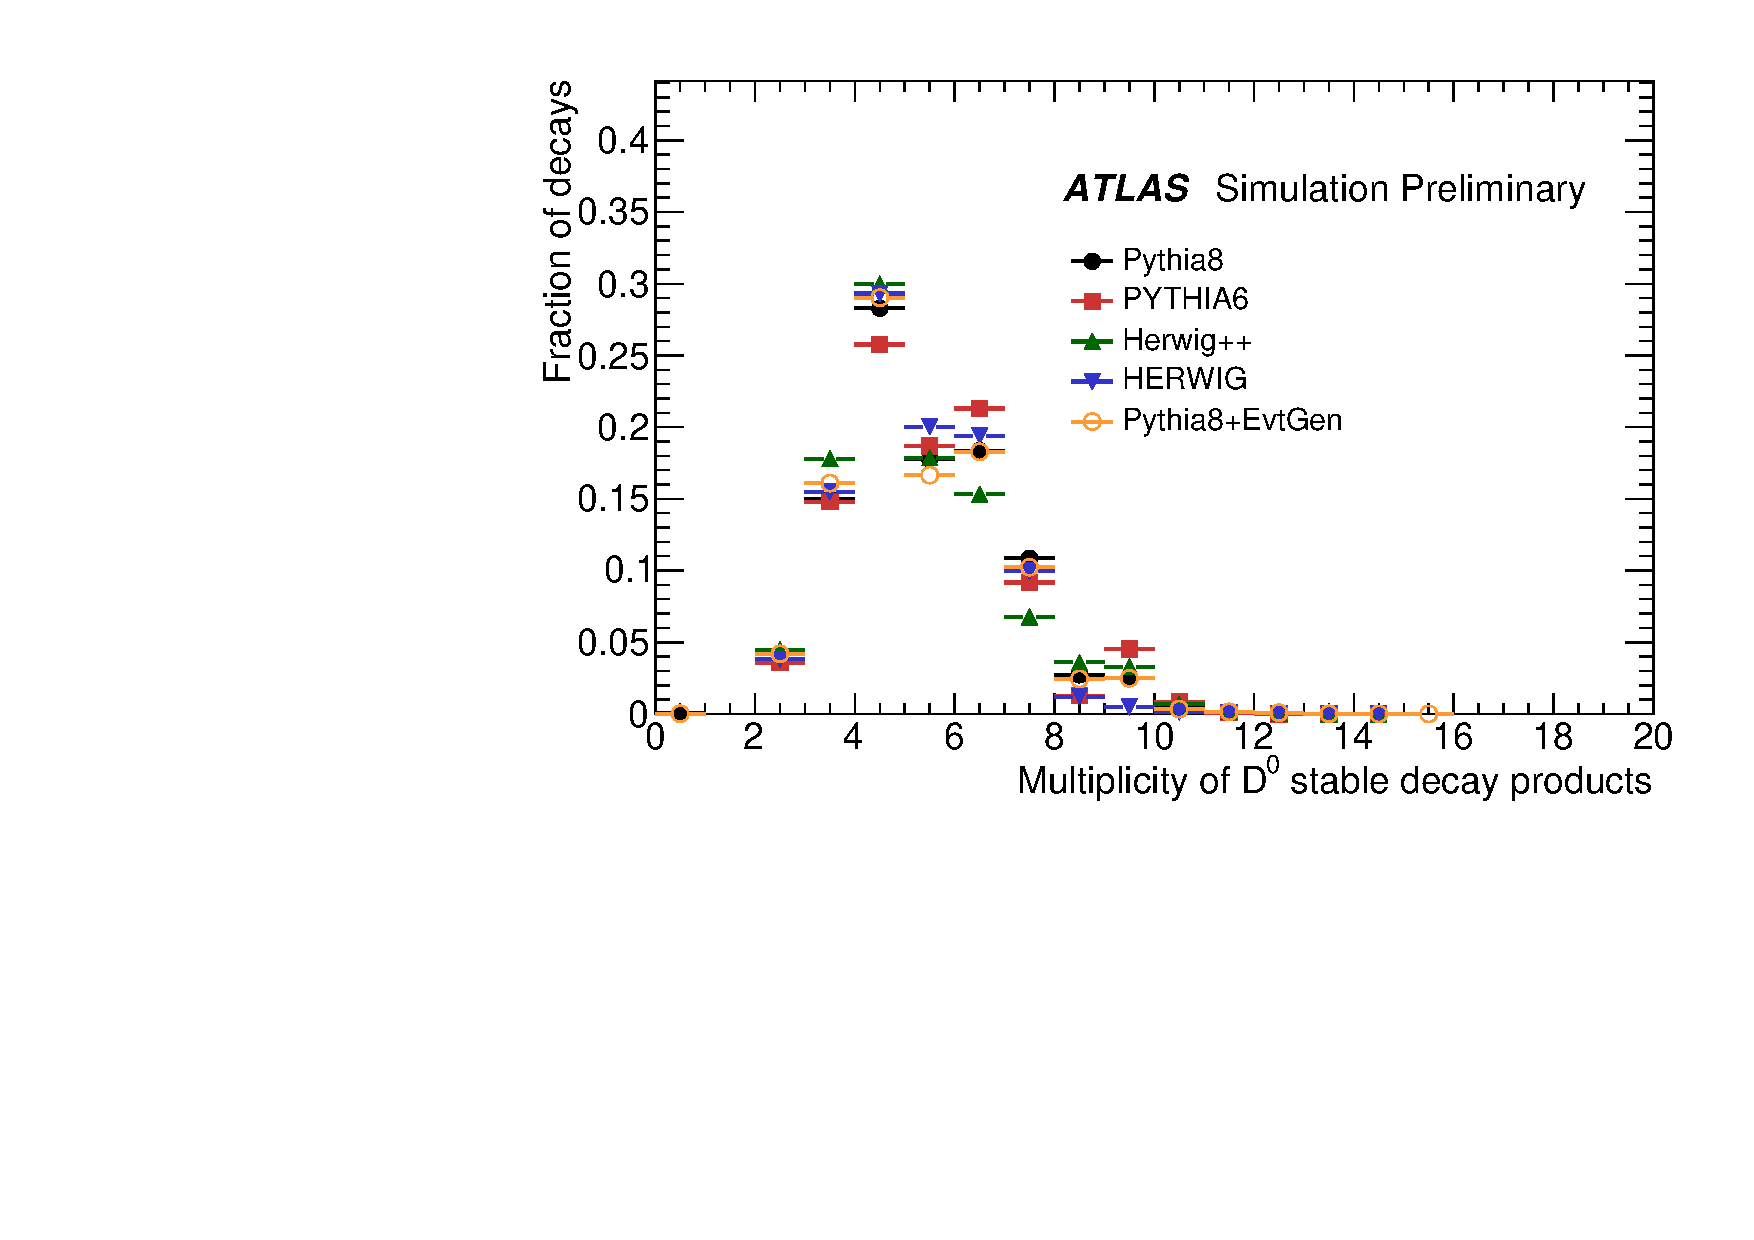
\includegraphics[width=\textwidth]{evtgen/figures/EvtGen/D0/h_species_multiplicity.pdf}
\end{subfigure}
\begin{subfigure}[]{0.45\textwidth}
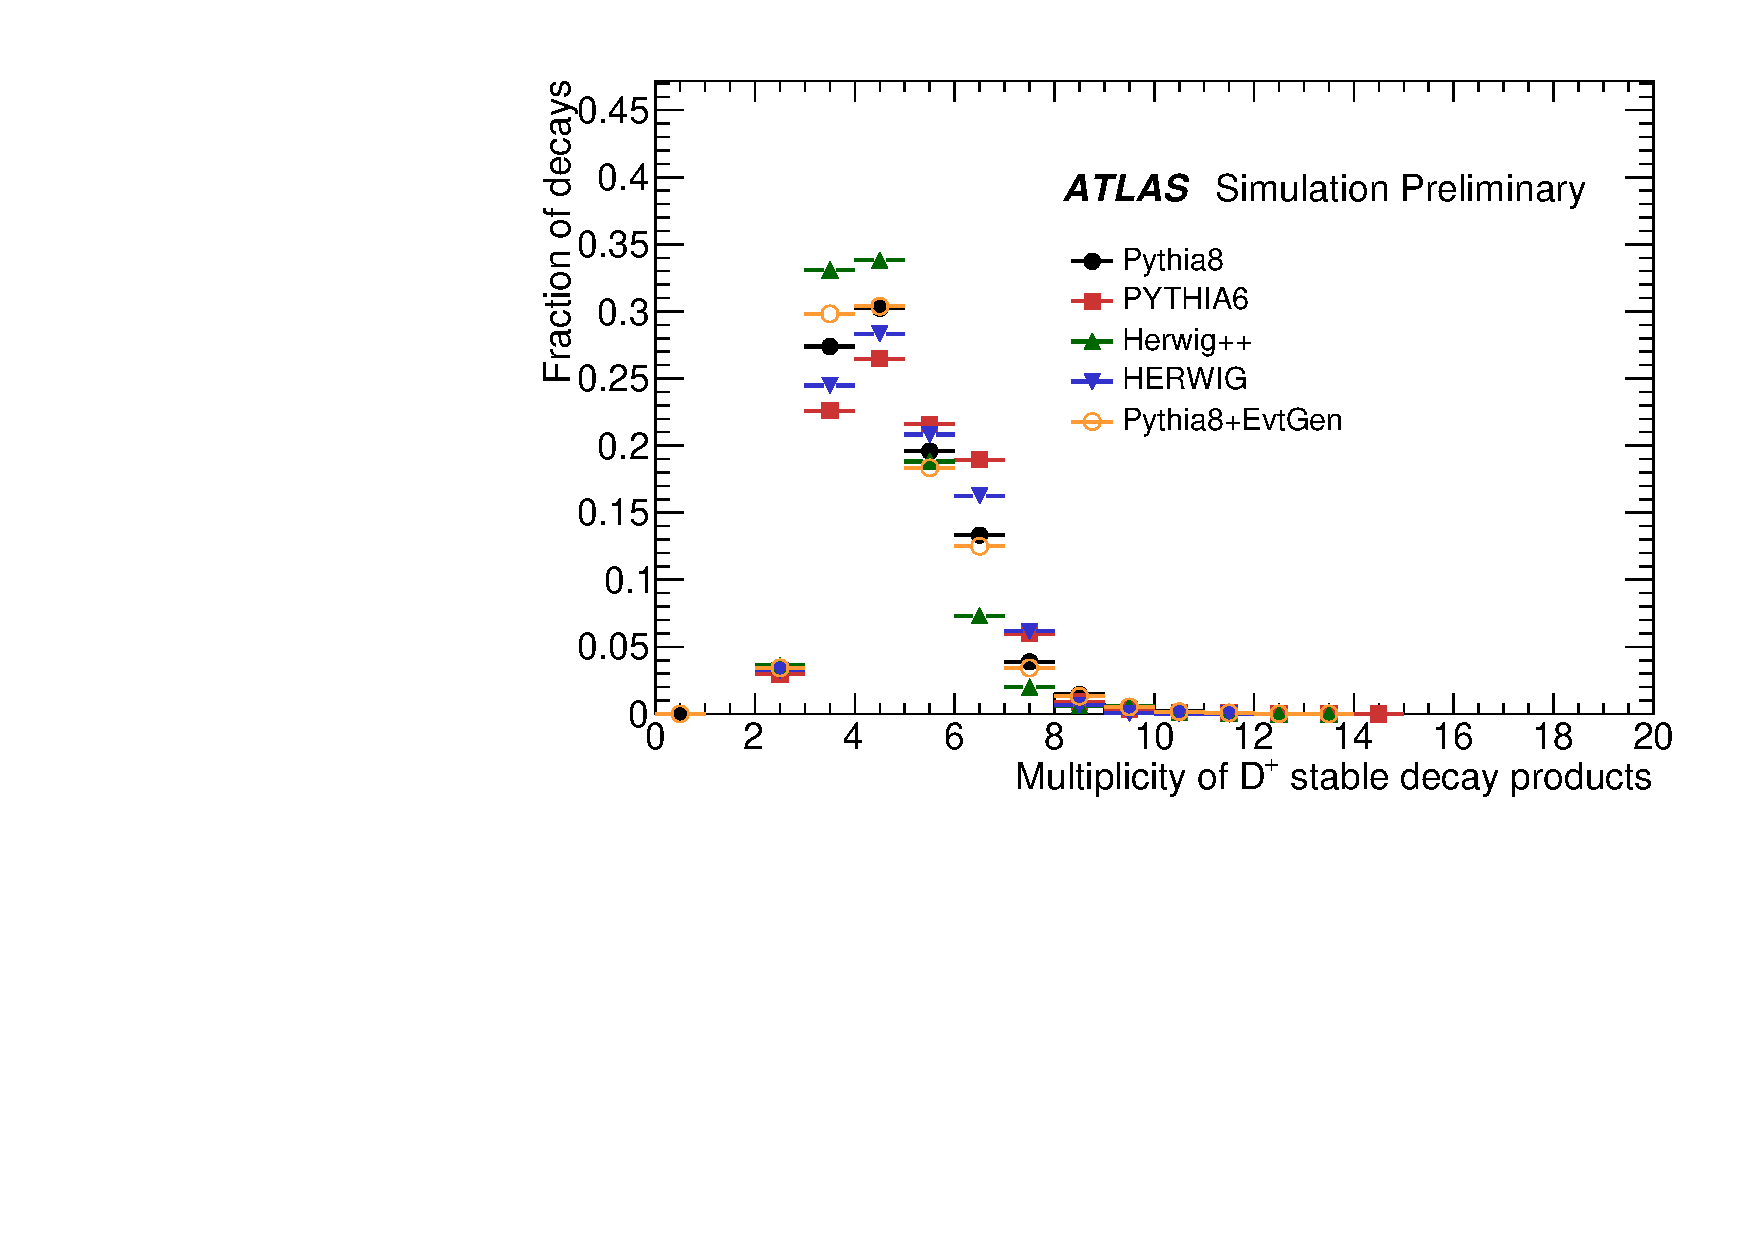
\includegraphics[width=\textwidth]{evtgen/figures/EvtGen/D+/h_species_multiplicity.pdf}
\end{subfigure}\\
\begin{subfigure}[]{0.45\textwidth}
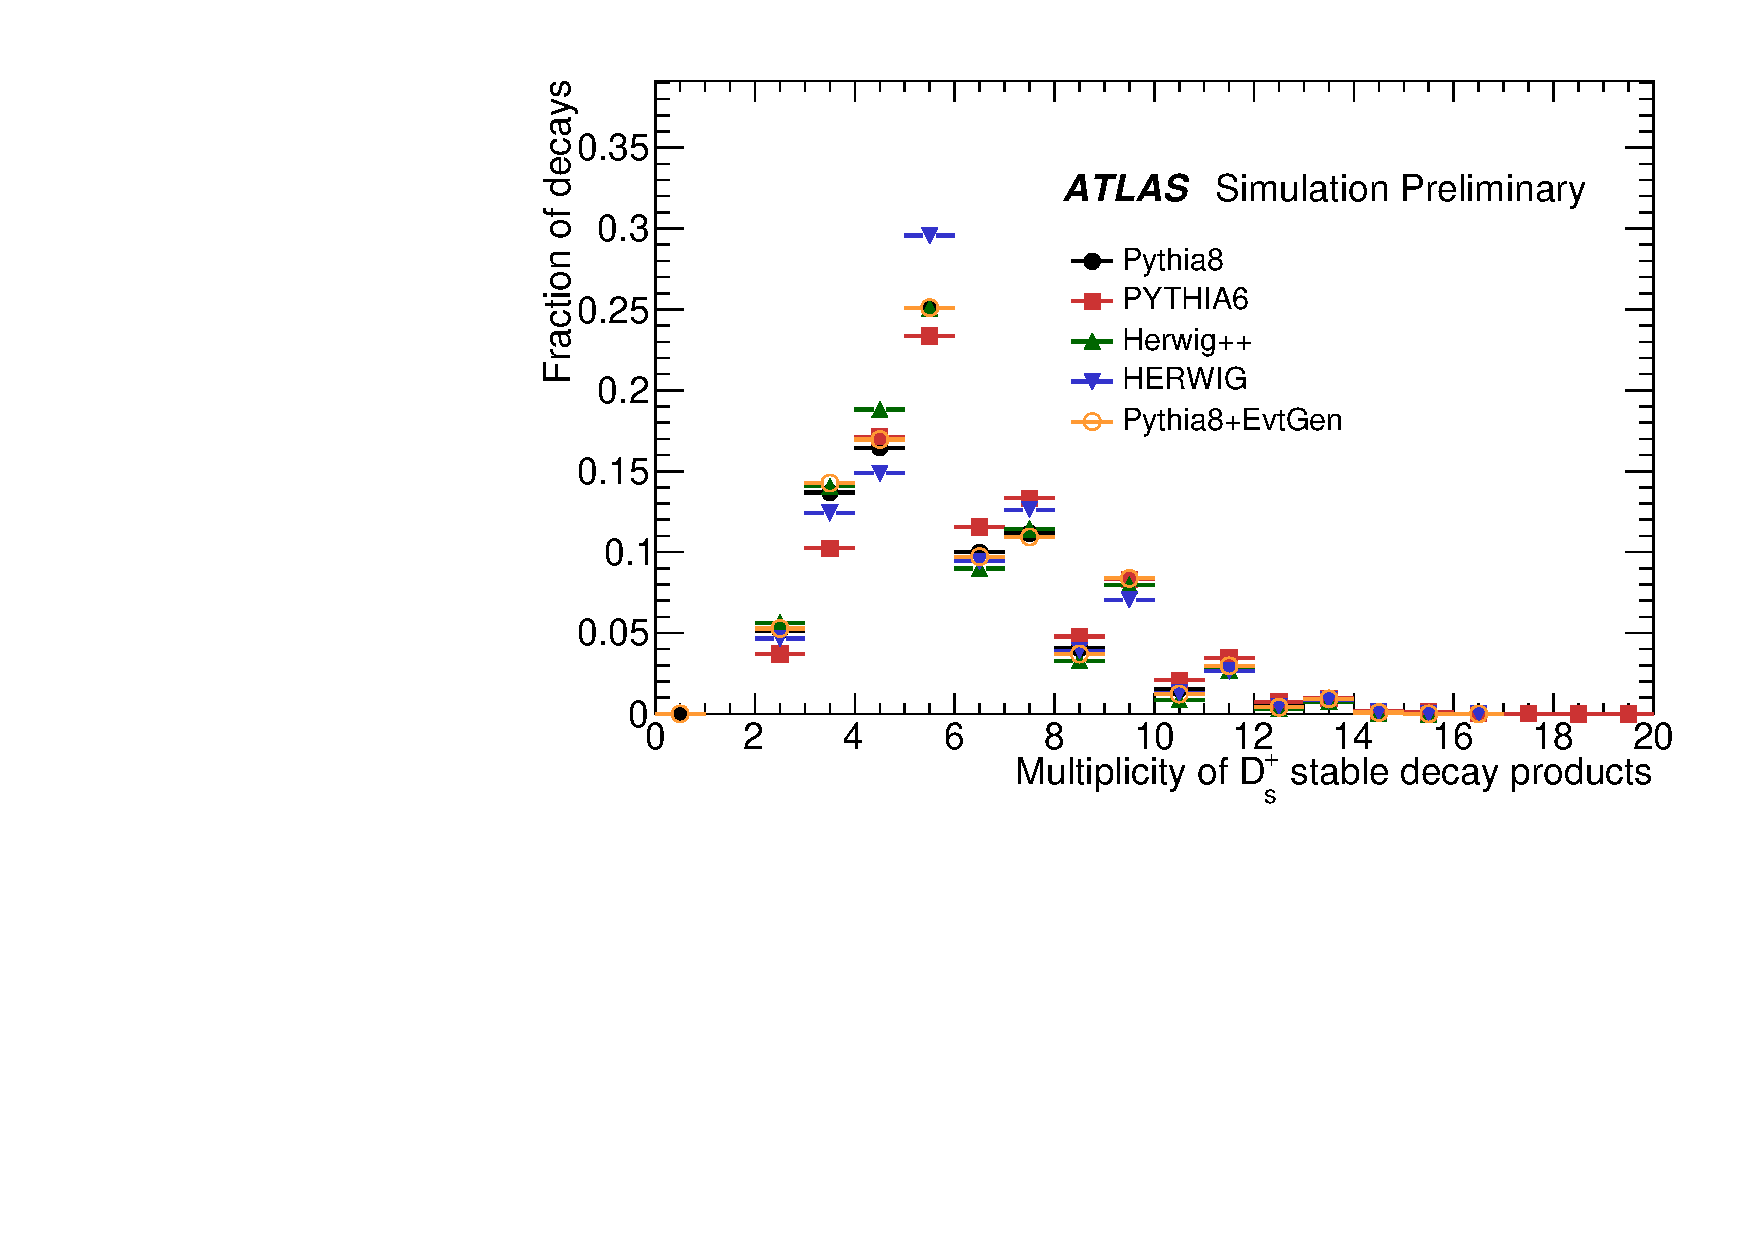
\includegraphics[width=\textwidth]{evtgen/figures/EvtGen/Ds+/h_species_multiplicity.pdf}
\end{subfigure}
\begin{subfigure}[]{0.45\textwidth}
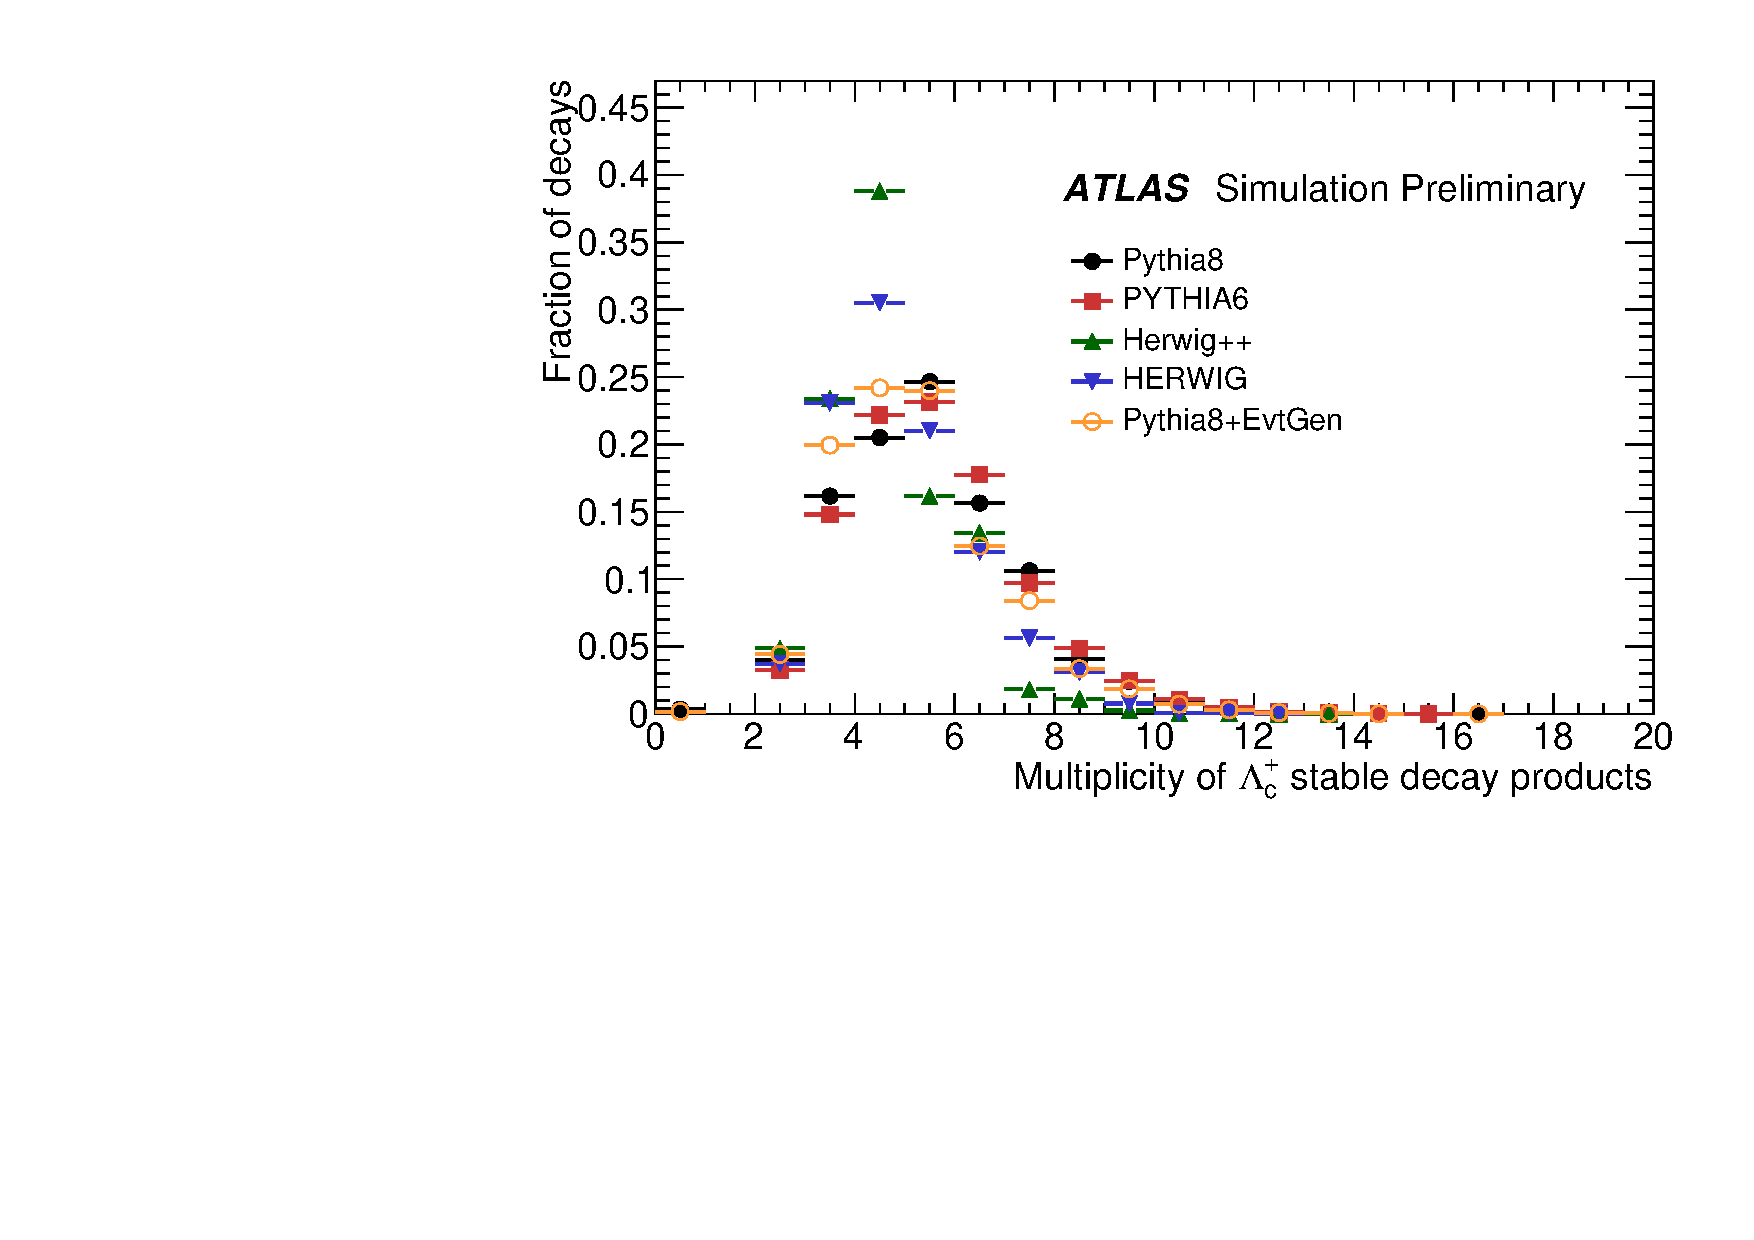
\includegraphics[width=\textwidth]{evtgen/figures/EvtGen/Lambdac+/h_species_multiplicity.pdf}
\end{subfigure}
\caption{Comparison of the multiplicity of stable decay products for the weakly decaying 
charm hadrons 
(a) \Dzero,~ (b) \Dplus,~ (c) \Ds\ and (d) \Lc~ in \PythiaE\,~ \Pythia\, \newline  \Herwigpp\, ~\Herwig\ and \EvtGen.
A stable particle is defined
as a particle with a proper lifetime $c\tau_{0}>10$~mm. }
\label{fig:cmult}
\end{figure}




\begin{table}
\begin{center}
\begin{tabular}{|c|c|c|c|c|c|}
\hline
\multicolumn{6}{|c|}{Multiplicity of charged, stable decay products} \\
\hline \hline
Particle & \PythiaE & \Pythia & \Herwigpp & \Herwig & \PythiaE +\EvtGen \\ \hline
\Bo & $ 4.928 \pm 0.006 $ & $ 5.336 \pm 0.006 $ & $ 4.475 \pm 0.005 $ & $ 4.690 \pm 0.005 $ & $ 4.853 \pm 0.004 $ \\
\Bp & $ 4.754 \pm 0.005 $ & $ 5.102 \pm 0.006 $ & $ 4.435 \pm 0.005 $ & $ 4.636 \pm 0.005 $ & $ 4.750 \pm 0.004 $\\
\Bs & $ 4.661 \pm 0.012 $ & $ 5.136 \pm 0.013 $ & $ 4.319 \pm 0.010 $ & $ 4.665 \pm 0.011 $ & $ 4.623 \pm 0.008 $ \\
$\Lambda_b^{0}$ & $ 4.976 \pm 0.018 $ & $ 5.010 \pm 0.015 $ & $ 4.153 \pm 0.011 $ & $ 4.280 \pm 0.012 $ & $ 4.957 \pm 0.013 $ \\
\Dzero & $ 2.215 \pm 0.003 $ & $ 2.273 \pm 0.003 $ & $ 2.182 \pm 0.003 $ & $ 2.263 \pm 0.003 $ & $ 2.208 \pm 0.002 $  \\
\Dplus & $ 1.965 \pm 0.003 $ & $ 2.161 \pm 0.004 $ & $ 1.920 \pm 0.004 $ & $ 2.154 \pm 0.005 $ & $ 1.958 \pm 0.002 $ \\
\Ds & $ 2.103 \pm 0.007 $ & $ 2.410 \pm 0.008 $ & $ 2.129 \pm 0.008 $ & $ 2.476 \pm 0.009 $ & $ 2.102 \pm 0.005 $ \\
$\Lambda_c^{+}$ & $ 2.222 \pm 0.010 $ & $ 2.353 \pm 0.009 $ & $ 2.004 \pm 0.008 $ & $ 1.980 \pm 0.006 $ & $ 2.193 \pm 0.007 $ \\ \hline
\end{tabular}
\caption{Mean number of charged, stable decay products for the weakly decaying 
bottom and charm hadrons species
in \PythiaE\,~ \Pythia\, \newline  \Herwigpp\, ~\Herwig\ and \EvtGen.  A stable particle is defined
as a particle with a proper lifetime $c\tau_{0}>10$~mm.}
\label{t:charge}
\end{center}
\end{table}


\begin{table}
\begin{center}
\begin{tabular}{|c|c|c|c|c|c|}
\hline
\multicolumn{6}{|c|}{Multiplicity of stable decay products} \\
\hline \hline
Particle & \PythiaE & \Pythia & \Herwigpp & \Herwig & \PythiaE +\EvtGen \\
\hline
\Bo & $ 11.379 \pm 0.012 $ & $ 11.939 \pm 0.013 $ & $ 9.919 \pm 0.011 $ & $ 10.339 \pm 0.012 $ & $ 10.982 \pm 0.009 $  \\
\Bp & $ 11.527 \pm 0.013 $ & $ 12.263 \pm 0.014 $ & $ 10.283 \pm 0.012 $ & $ 10.550 \pm 0.012 $ & $ 11.250 \pm 0.009 $ \\
\Bs & $ 11.933 \pm 0.030 $ & $ 12.552 \pm 0.032 $ & $ 10.516 \pm 0.024 $ & $ 10.706 \pm 0.024 $ & $ 11.631 \pm 0.021 $ \\
$\Lambda_b^{0}$ & $ 11.220 \pm 0.040 $ & $ 11.298 \pm 0.034 $ & $ 9.376 \pm 0.024 $ & $ 10.060 \pm 0.026 $ & $ 10.772 \pm 0.027 $ \\
\Dzero & $ 4.920 \pm 0.006 $ & $ 5.002 \pm 0.006 $ & $ 4.784 \pm 0.006 $ & $ 4.748 \pm 0.007 $ & $ 4.853 \pm 0.004 $ \\
\Dplus & $ 4.344 \pm 0.007 $ & $ 4.554 \pm 0.008 $ & $ 4.053 \pm 0.007 $ & $ 4.437 \pm 0.009 $ & $ 4.265 \pm 0.005 $  \\
\Ds & $ 5.564 \pm 0.017 $ & $ 5.842 \pm 0.019 $ & $ 5.393 \pm 0.019 $ & $ 5.548 \pm 0.019 $ & $ 5.500 \pm 0.012 $ \\
$\Lambda_c^{+}$ & $ 5.007 \pm 0.021 $ & $ 5.100 \pm 0.019 $ & $ 4.219 \pm 0.015 $ & $ 4.485 \pm 0.013 $ & $ 4.751 \pm 0.014 $  \\ 
\hline
\end{tabular}
\caption{Mean number of stable decay products for the weakly decaying 
bottom and charm hadrons species
in \PythiaE\,~ \Pythia\, \newline  \Herwigpp\, ~\Herwig\ and \EvtGen.  A stable particle is defined
as a particle with a proper lifetime $c\tau_{0}>10$~mm.}
\label{t:mult}
\end{center}
\end{table}




